%%%%%%%%%%%%%%%%%%%% book_it.tex %%%%%%%%%%%%%%%%%%%%%%%%%%%%%
%
% Esempio di file principale per i capitoli della vostra  "monografia"
%
% Usare questo file come template per il vostro documento.
%
%%%%%%%%%%%%%%%% Springer-Verlag %%%%%%%%%%%%%%%%%%%%%%%%%%


% CONSIGLIATO
%%%%%%%%%%%%%%%%%%%%%%%%%%%%%%%%%%%%%%%%%%%%%%%%%%%
\documentclass[envcountsame,envcountchap]{svmono}

% scegliere le opzioni per []  come richiesto dalla lista 
% nella Reference Guide, Sez. 2.2

\usepackage{makeidx}         % permette di generare l'indice
\usepackage{graphicx}        % pacchetto grafico standard LaTeX 
                             % per l'inclusione di file immagine
\graphicspath{{./}{Figure/}}
\usepackage{amsfonts,amsmath,amssymb}
\usepackage{multicol}        % usato per l'indice a due colonne
\usepackage{subcaption}
\usepackage{cancel}
\usepackage{quoting}
\usepackage[bottom]{footmisc}% mette le note a pie' di pagina
\usepackage[italian]{babel}
\usepackage{mathtools}
% etc.
% si veda la lista di ulteriori pacchetti utili 
% nella Reference Guide, Sez. 2.3, 3.1-3.3

\def\theoremname{Teorema}
\makeindex             % usato per l'indice degli argomenti 
                       % si prega di usare lo stile svind.ist con 
                       % il vostro programma makeindex


%%%%%%%%%%%%%%%%%%%%%%%%%%%%%%%%%%%%%%%%%%%%%%%%%%%%%%%%%%%%%%%%%%%%%

\begin{document}

\author{Armenante Davide}
\title{Progetto di macchine\\
%{\small SPIN Springer internal project number, se noto}
}
\subtitle{Appunti del corso}
\date{2020}
\maketitle

\frontmatter%%%%%%%%%%%%%%%%%%%%%%%%%%%%%%%%%%%%%%%%%%%%%%%%%%%%%%

%%%%%%%%%%%%%%%%%%%%%%% dedic.tex %%%%%%%%%%%%%%%%%%%%%%%%%%%%%%%%%
%
% Esempio di dedica
%
% Usare questo file come template per il vostro documento.
%
%%%%%%%%%%%%%%%%%%%%%%%% Springer-Verlag %%%%%%%%%%%%%%%%%%%%%%%%%%

\thispagestyle{empty}
\vspace*{3.5cm}
\begin{flushright}

% scrivere qui
{\large Prego comunque...}

\end{flushright}




%%%%%%%%%%%%%%%%%%%%%% pref_it.tex %%%%%%%%%%%%%%%%%%%%%%%%%%%%%%%%%%%%%
%
% Esempio di prefazione
%
% Usare questo file come template per il vostro documento.
%
%%%%%%%%%%%%%%%%%%%%%%%% Springer-Verlag %%%%%%%%%%%%%%%%%%%%%%%%%%

\preface

Prima che il lettore si immerga in questa appassionante lettura vorrei fare due precisazioni. L'impaginazione è tanto figa quanto il libro è scritto male, non si tratta di un elaborato professionale ma di appunti presi a lezione. Apprezzate però, tutte le immagini sono state rifatte vettorialmente.


%% Si prega di  "firmare" la prefazione
\vspace{1cm}
\begin{flushright}\noindent
Trieste,\hfill {\it Davide Armenante}\\
02, 2020\hfill\\
\end{flushright}




\tableofcontents


\mainmatter%%%%%%%%%%%%%%%%%%%%%%%%%%%%%%%%%%%%%%%%%%%%%%%%%%%%%%%
\chapter{Richiami teorici}
\section{Teoria della similitudine}
L’applicazione della teoria della similitudine costituisce un primo e potente strumento della progettazione, in particolar modo per quanto riguarda le turbomacchine. La teoria della similitudine permette di risolvere diversi problemi:
\begin{itemize}
\item[$-$] note le prestazioni di una macchina che ha determinate dimensioni,
si possono ricavare le prestazioni di una macchina geometricamente simile a quella considerata ma di diverse dimensioni nel dettaglio permette la realizzazione di prototipi in scala ridotta (esempio tipico: modellino della grande turbina idraulica che viene provato prima di procedere alla costruzione della macchina vera);
\item[$-$] nota una ben determinata condizione di funzionamento di una turbomacchina, come potrebbero essere le condizioni di progetto, si possono individuare altre condizioni di funzionamento ottenute variando la velocità di rotazione, la portata, oppure il lavoro scambiato (fluido/macchina);
\item[$-$] curve di prestazioni rilevate in determinate condizioni ambientali possono essere espresse in funzione di parametri che sono invarianti al variare delle condizioni ambientali stesse. Possiamo conoscere le prestazioni di una macchina operante in condizioni diverse (ad esempio un compressore sul livello del mare ad agosto e in montagna a Natale);
\end{itemize}
Accanto a tutti questi aspetti riguardanti la capacità di predire le prestazioni di una macchina, si ritrova anche un ausilio al designer in sede di progettazione. Con la teoria della similitudine si può stabilire in maniera semplice e veloce fin da subito quale sarà il tipo di macchina migliore da usare, quale sarà la sua geometria di base e quali le dimensioni generali. Grazie a ciò si riesce a sfruttare l’esperienza già maturata nella progettazione, sviluppo e test di altre macchine simili. Possedere un database ricco di informazioni relative a macchine pregresse risulta essere un vantaggio progettuale non di poco conto.


ll teorema di Buckingham (conosciuto anche come teorema pi greco), dovuto al fisico statunitense Edgar Buckingham, afferma:
\begin{quoting}
Dato un problema descritto da un certo numero di equazioni in cui siano presenti $n$ variabili fisiche, se le dimensioni fondamentali di queste variabili sono $x$ allora il problema può essere completamente descritto da $n - x$ variabili adimensionali.
\end{quoting}
Per studiare il comportamento di una turbomacchina si definisce il seguente funzionale.
\begin{equation}
f(D_i,l_j,\dot{m},w,L_i,\mu,a_{01},\rho_{01})=0
\end{equation}
Con\\
$D_i$: serie di diametri rilevanti;\\
$l_j$: serie di lunghezze rilevanti;\\
$\dot{m}$: portata in massa;\\
$w$: velocità angolare;\\
$L_i$: lavoro ideale scambiato tra macchina e fluido per unità di massa;\\
$\mu$: viscosità dinamica del fluido;\\
$a_{01}$: velocità del suono all'ingresso in condizioni di ristagno;\\
$\rho_{01}$: densità del fluido.
\begin{equation}
Re= \frac{\rho_{01} w D^2}{\mu}
\end{equation}
\begin{equation}
Ma= \frac{w D}{a_{01}}
\end{equation}
Si evidenzia che tutti gli argomenti del funzionale sono descritti da una combinazione delle tre grandezze fondamentali M L T, ovvero massa lunghezza e tempo. Tenendo presente ciò è possibile adimensionalizzare gli argomenti del funzionale ottenendo una nuova espressione per lo stesso.

In una macchina termica in cui il fluido cambia le proprietà nei vari punti della macchina per definire la densità o la velocità del suono devo fissare
convenzionalmente una condizione rispetto alla quale vado a valutare quella
proprietà. 

Una condizione di riferimento che viene spesso adottata (non è
l’unica) potrebbe essere quella di valutare queste quantità nelle condizioni
totali all’ingresso della macchina (cioè condizioni valutate immaginando il fluido in quiete) che possiamo indicare con il pedice $01$ ($0$: condizioni totali o di ristagno; $1$: condizioni di ingresso).

Si può allo stesso modo definire le cifre di flusso $\Phi$ e di pressione $\psi$ andando ad adimensionalizzare rispettivamente la portata e il lavoro unitario:
\begin{equation}
\phi = \frac{\dot{m}}{w D^3} \left( =\frac{Q}{w D^3} \right)
\end{equation}
\begin{equation}
\psi = \frac{L_i}{\rho_{01} w^2 D^2}
\end{equation}
Il funzionale può essere espresso quindi secondo i numeri adimensionali:
\begin{equation}
f(\pi_i,\pi_j,\phi,\psi,Re,Ma)=0
\end{equation}
Si può semplificare sotto le ipotesi di geometria simile.
\begin{equation}
f(\phi,\psi,Re,Ma)=0
\end{equation}
Supponendo di confrontare due macchine se queste hanno le gli stessi valori di $\pi_i$ e $\pi_j$, allora la geometria tra le due macchine sarà da considerarsi simile e sotto queste ipotesi il funzionale si semplifica come di seguito:
\begin{figure}
\centering
  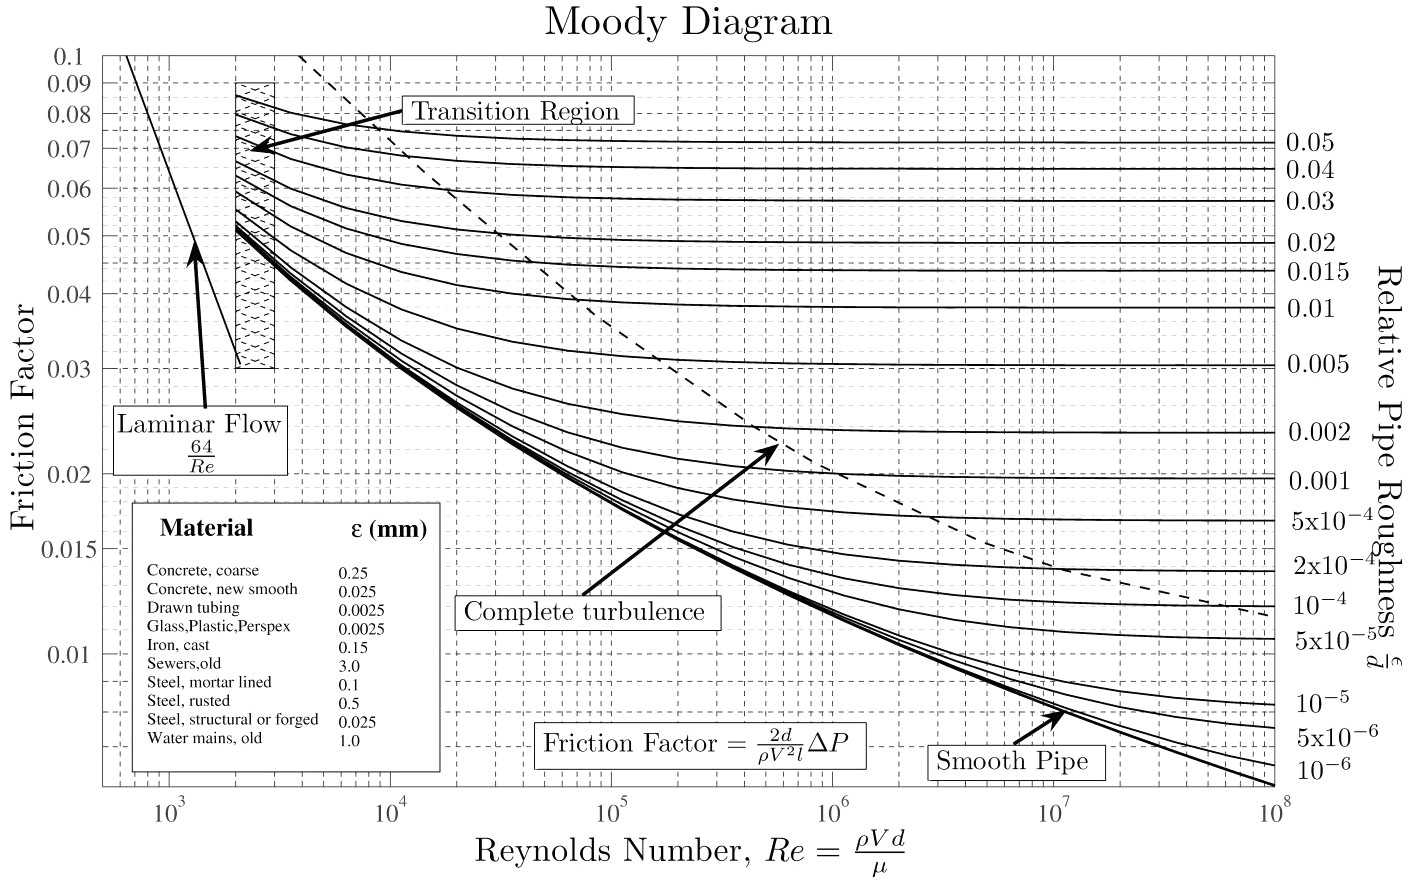
\includegraphics[width=\textwidth]{fig/moody.jpg}
\caption{}
\label{fig:moody}
\end{figure}
Guardando il diagramma di Moody in figura \ref{fig:moody}, in ascisse è presente $Re$ ed in ordinate il coefficiente di perdita di carico del nostro tubo $\xi$. Le scale sono logaritmiche. Il legame tra $\xi$ e $Re$, per bassi numeri di Reynolds, è rappresentato da una retta. Poi si ha una zona di transizione non ben definita ed infine una serie di linee a rugosità relativa costante $\epsilon/D$ (con $\epsilon$ rugosità media).

Nel primo tratto di legame lineare si ha una corrente laminare. Il tratto tratteggiato è un tratto nel quale, in condizioni sperimentali assolutamente controllate, è possibile mantenere un flusso laminare ma altamente instabile. In condizioni di flusso turbolento la perdita di carico dipende dalla rugosità.
Possiamo inoltre osservare che se consideriamo un solo valore di rugosità relativa la curva presenta una certa pendenza fino ad un certo valore di $Re$ (limite o critico) e poi diventa orizzontale. Sotto le ipotesi di moto turbolento pienamente sviluppato possiamo quindi trascurare l’influenza di Reynolds nel funzionale. Va ovviamente considerato che le rugosità relative di una macchina grande saranno in genere diverse da quelle che si possono ottenere con macchine piccole, quindi bisogna tenerlo presente. Variazioni anche grandi del numero di Reynolds, purché in regime di moto turbolento completamente sviluppato (corrispondenti a valori di Re molto elevati), non influenzano le prestazioni della mia macchina.

Se il numero di Reynolds è superiore ad un certo valore limite il coefficiente di perdita di carico è indipendente da $Re$. Se trasferiamo questa osservazione alla turbomacchina si può verificare sperimentalmente che se $Re$ è molto elevato questo potrà anche variare ma le prestazioni non ne saranno influenzate. Variazioni anche grandi del numero di Reynolds purchè siano nel
campo di $Re$ molto elevato, non influenzano le prestazioni della mia macchina.
\begin{equation}
f(\phi,\psi,Ma)=0
\end{equation}
In seguito, si aggiungerà una perdita sul modello in quanto il rendimento di una macchina piccola sarà sempre inferiore al rendimento di una macchina grande.

In ultimo se si considerano i fenomeni di comprimibilità trascurabili, si può trascurare anche il numero di Mach, equivalentemente si fa l'ipotesi $Ma\;<\;0.3$.
\begin{align*}
f(\Phi,\psi)=0
\end{align*}
Dotando la pompa di un sensore di pressione, giri e portata, posso andare a definire una curva di prestazione adimensionale.
Si definiscono orea le tre componenti del vettore velocità:
\begin{itemize}
\item[$c$]: velocità assoluta;
\item[$w$]: velocità relativa;
\item[$u$]: velocità periferica;
\end{itemize}
Naturalmente affinchè le macchine operino in condizioni di similitudine devono, per definizione, avere $\phi$ e $\psi$ uguali. 
\begin{equation}
\phi=\frac{Q}{w D^3} \propto \frac{c_m}{u}
\end{equation}

\begin{equation}
\psi = \frac{L_i}{w^2 D^2} \propto \frac{c_u}{u}
\end{equation}
Quindi, assegnato $D$, la cifra di flusso è proporzionale alla velocità meridiana e inversamente proporzionale a $u$ dove $u= \omega \times r$. La variazione di $c_u$ corrisponde alla variazione dell'energia cinetica a valle della macchina. 

Mantenere $\phi$ e $\psi$ uguali significa avere triangoli di velocità simili (vedi la figura \ref{fig:tria}).
\begin{figure}
\centering
  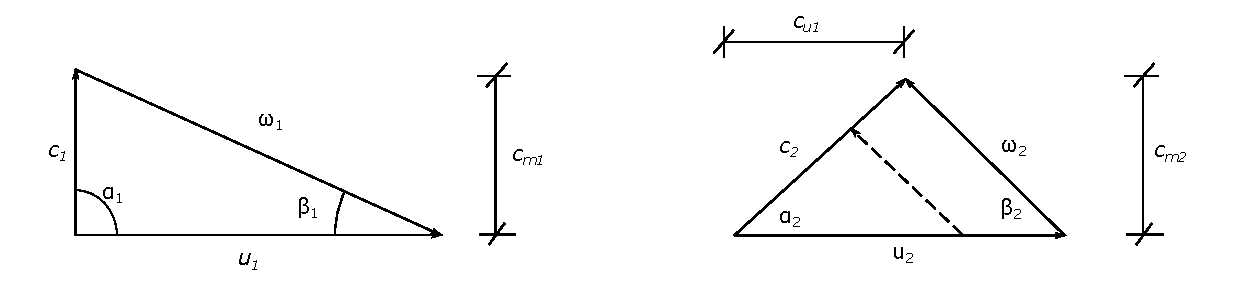
\includegraphics[width=.8\textwidth]{fig/triang.pdf}
\caption{}
\label{fig:tria}
\end{figure}
Consideriamo il caso di una macchina idraulica e vediamo come possiamo trovare il luogo dei punti di funzionamento simili sul piano delle prestazioni e quindi come le curve di prestazioni adimensionali stanno in rapporto con le curve di prestazioni dimensionali.

Se rileviamo le prestazioni di una pompa otteniamo la curva di funzionamento caratteristica (diagramma prevalenza-portata) per un certo valore della velocità di rotazione (figura \ref{fig:hq}).
\begin{figure}[h!]
\centering
  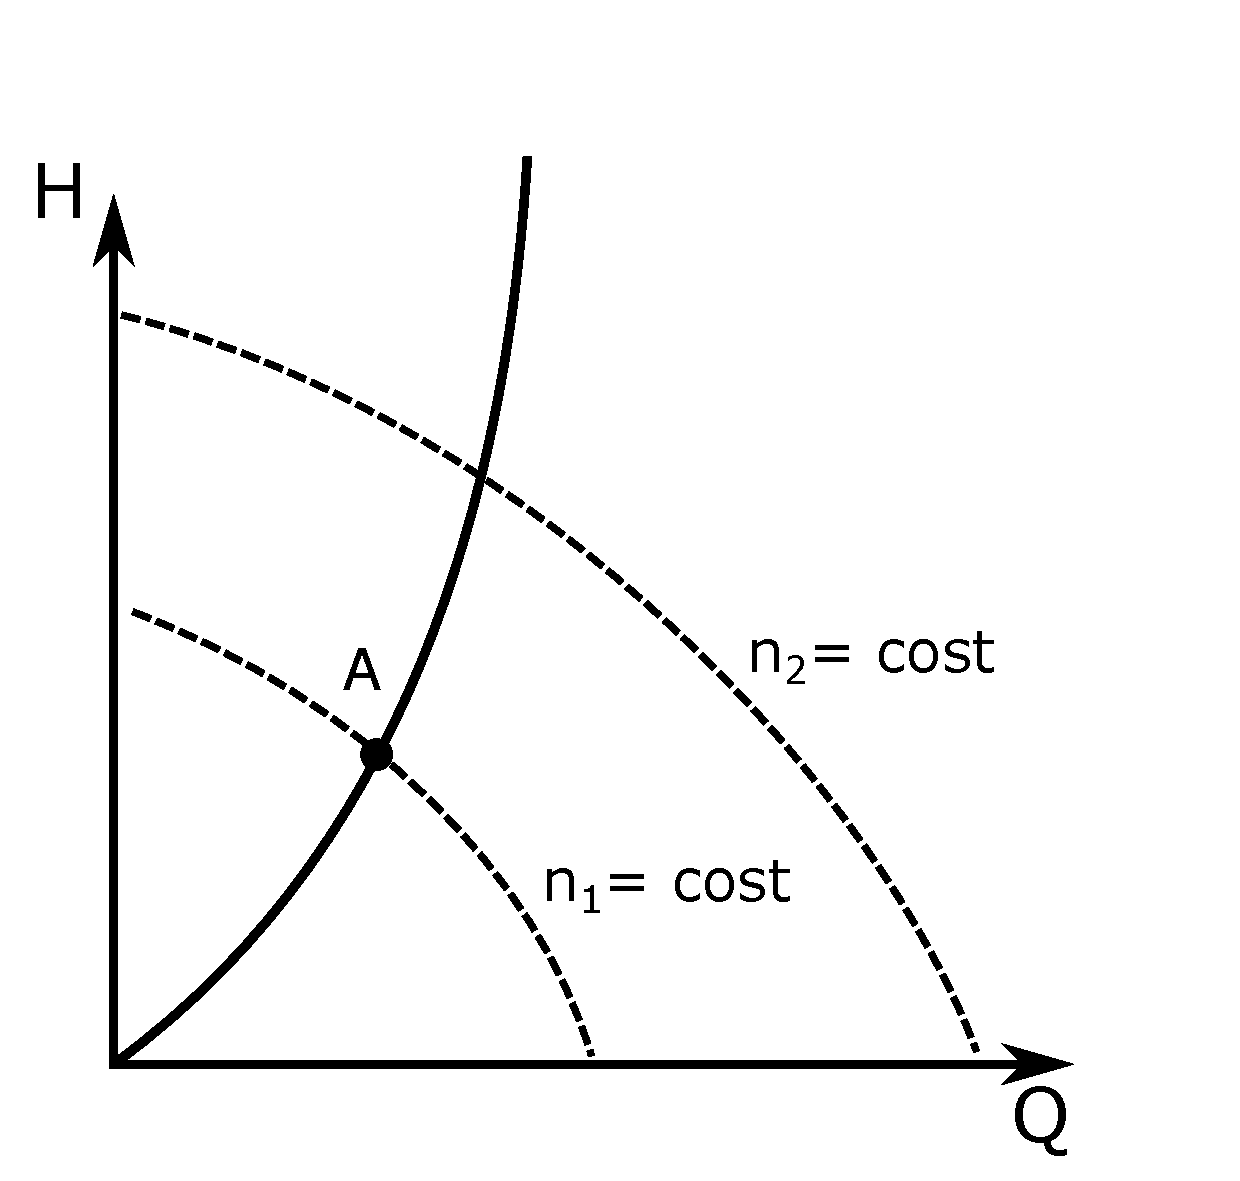
\includegraphics[width=.3\textwidth]{fig/hq.pdf}
\caption{}
\label{fig:hq}
\end{figure}
Queste sono curve espresse in funzione di grandezze dimensionali, ma andando ad adimensionalizzare si possono ottenere tali curve in funzione delle relative cifre di pressione e di flusso.  Si consideri un punto di funzionamento $A$, il luogo dei punti di funzionamento simili ad $A$ sarà caratterizzato dal fatto di avere stessi $\phi$ e $\psi$.

Considerando quindi il generico punto $x$ posso scrivere
\begin{equation}
\phi = \frac{Q}{w D^3}= \frac{Q_x}{w_x D^3}
\end{equation}
Considerando una macchina con lo stesso diametro posso scrivere
\begin{equation}
\frac{Q_x}{Q}=\frac{w_x}{w} \; \Rightarrow \; Q_x = Q \frac{w_x}{w}
\end{equation}
Imponendo invece l'uguaglianza della cifra di pressione
\begin{equation}
\psi = \frac{gH}{w^2 D^2}= \frac{gH_x}{w_x^2 D^2}
\end{equation}
In questo modo si ottiene
\begin{equation}
H_x = H(\frac{w_x}{w})^2 = H(\frac{Q_x}{Q})^2 \Rightarrow H_x = \frac{H}{Q^2}Q_x^2
\end{equation}
Che è l'equazione di una parabola sul piano H-Q, passante per il punto A e per l'origine degli assi. 
Noto che il lavoro varia al variare del quadrato della velocità angolare mentre la portata varia linearmente. 
Ad ogni curva $\phi - \psi$ corrisponde una curva di rendimento, posso quindi individuare una coppia $\bar{\phi} - \bar{\psi}$ ottimale (figura \ref{fig:adim}).
\begin{figure}[h!]
\centering
  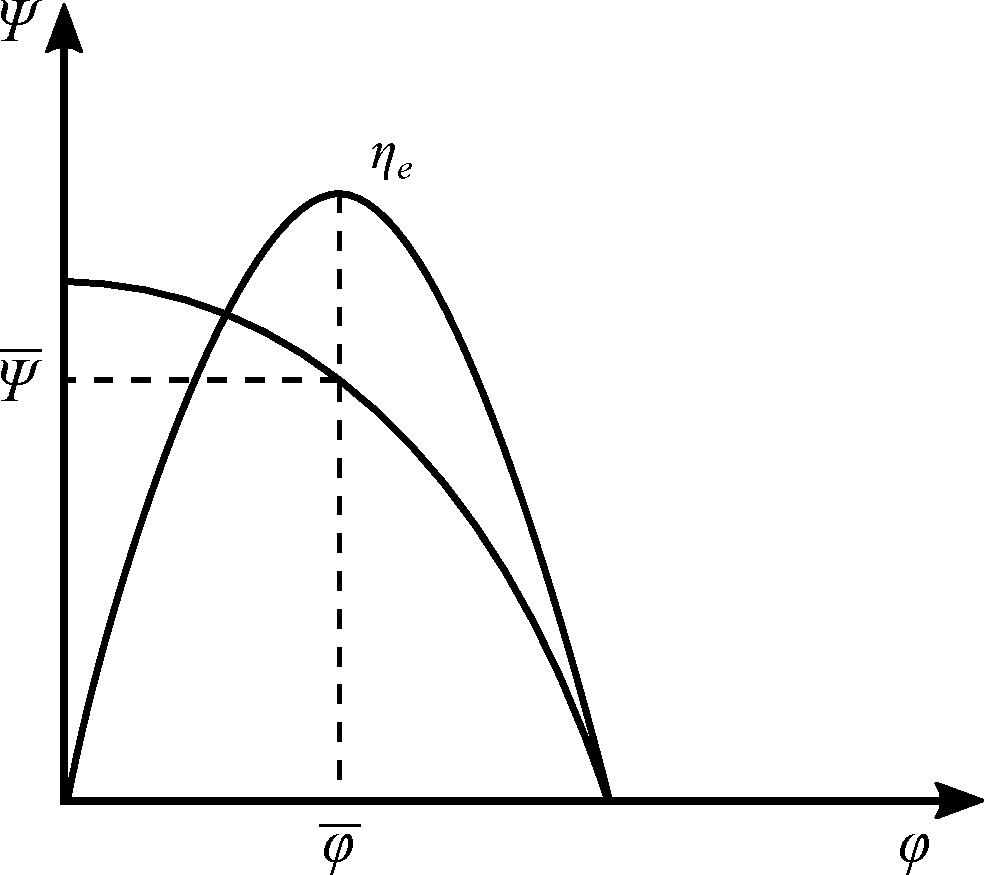
\includegraphics[width=.3\textwidth]{fig/adim.pdf}
\caption{}
\label{fig:adim}
\end{figure}
Posso anche definire il coefficiente di velocità periferica.
\begin{equation}
k_P = \frac{w D}{\sqrt{L_i}}
\end{equation}
Si tratta di una cifra che lega la velocità periferica della macchina al lavoro ideale della stessa.

Quando ho $\phi$ e $\psi$ posso definire una cifra di potenza adimensionalizzata come prodotto delle due.
\begin{equation}
\Lambda = \frac{P_e}{\rho w^3 D^5}
\end{equation}
Per macchina motrice
\begin{equation}
\Lambda = \phi \psi \eta_e
\end{equation}
Per macchina operatrice
\begin{equation}
\Lambda = \frac{\phi \psi}{\eta_e}
\end{equation}
Con la seguente espressione posso poi eliminare la caratteristica geometrica ottenere il numero specifico di macchina (o velocità specifica) che rappresenta una condizione di funzionamento lavoro-portata indipendente dalla dimensione della macchina. 
\begin{equation}
w_s = k = \phi^{1/2} \psi^{-3/4} = w \frac{\sqrt{Q}}{L_i^{3/4}}
\end{equation}
La forma della macchina varierà al variare di k . Avere dei k piccoli significa avere delle macchine nelle quali il termine di scambio di energia è prevalente rispetto al termine di portata. Questo numero permette, grazie all’esperienza storica (ovvero di tutti i dati che il progettista o la sua azienda possiedono in merito alle prestazioni di altre macchine), di classificare la forma geometrica di una macchina in base alle condizioni portata - lavoro.
\begin{figure}[h!]
\centering
  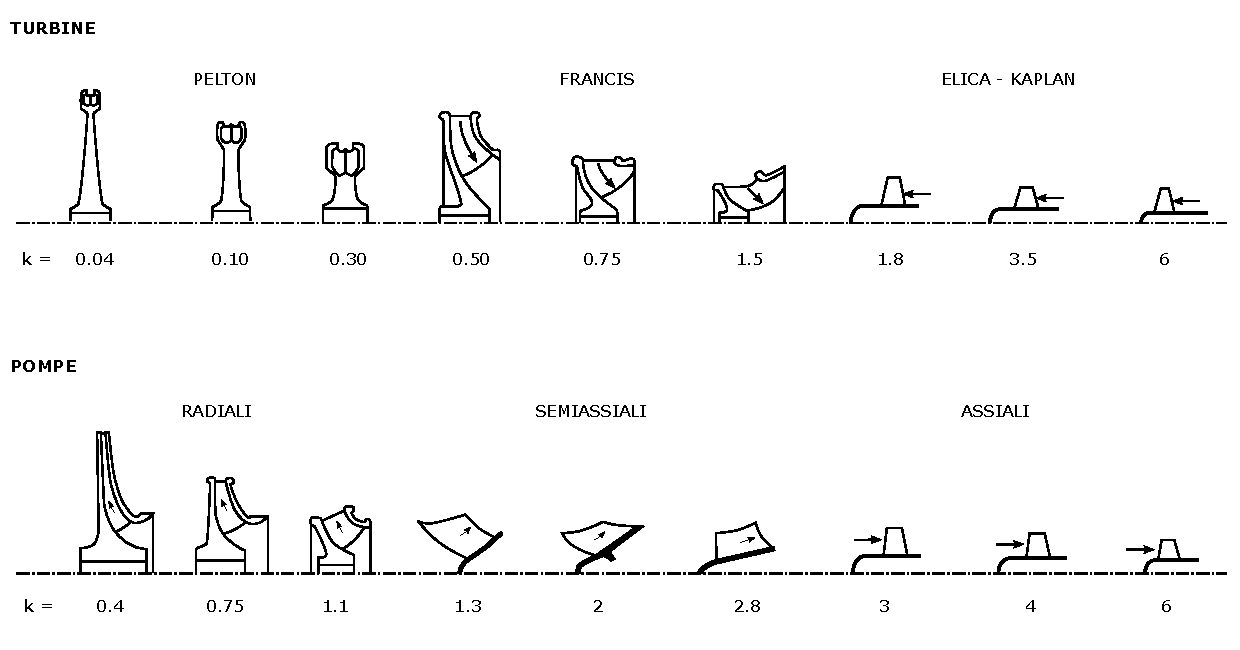
\includegraphics[width=\textwidth]{fig/numcar.pdf}
\caption{Variazione della forma delle giranti delle turbine idrauliche al variare del numero caratteristico di macchina.}
\label{fig:numcar}
\end{figure}
Queste cifre sono funzioni di k. Possono allora essere definite delle curve che riportano in ascissa il valore del numero caratteristico k e sulle ordinate i valori dei 4 rapporti.
Sfruttando l'esperienza possiamo analizzare le migliori macchine esistenti e vedere
quanto valgono per quelle macchine le cifre adimensionali $\pi_i$ , $\pi_j$ e diagrammarle in funzione di k . Facciamo un esempio concreto considerando una tipica macchina radiale (una pompa centrifuga) e consideriamo la sezione meridiana semplificata al massimo (figura \ref{fig:pala}).
\begin{figure}
\centering
\begin{minipage}{.5\textwidth}
  \centering
  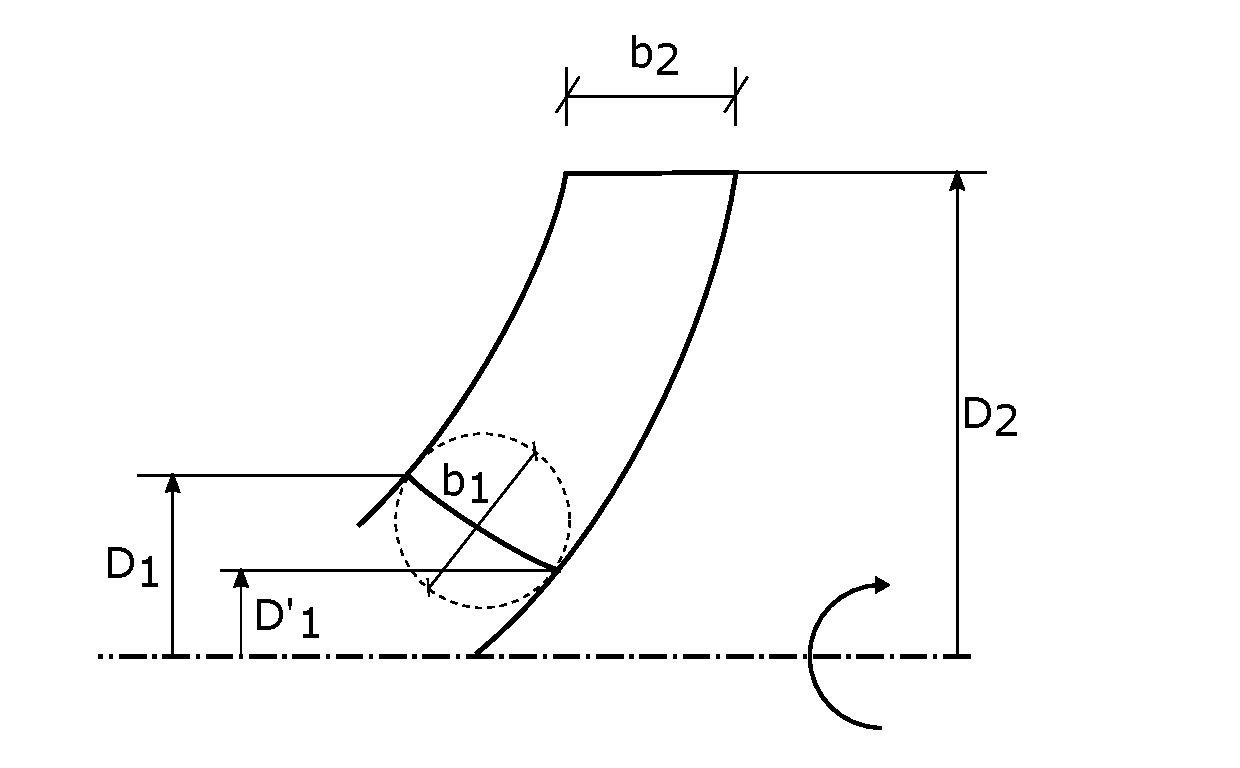
\includegraphics[width=.9\linewidth]{fig/pala.pdf}
  \captionof{figure}{}
  \label{fig:pala}
\end{minipage}%
\begin{minipage}{.5\textwidth}
  \centering
  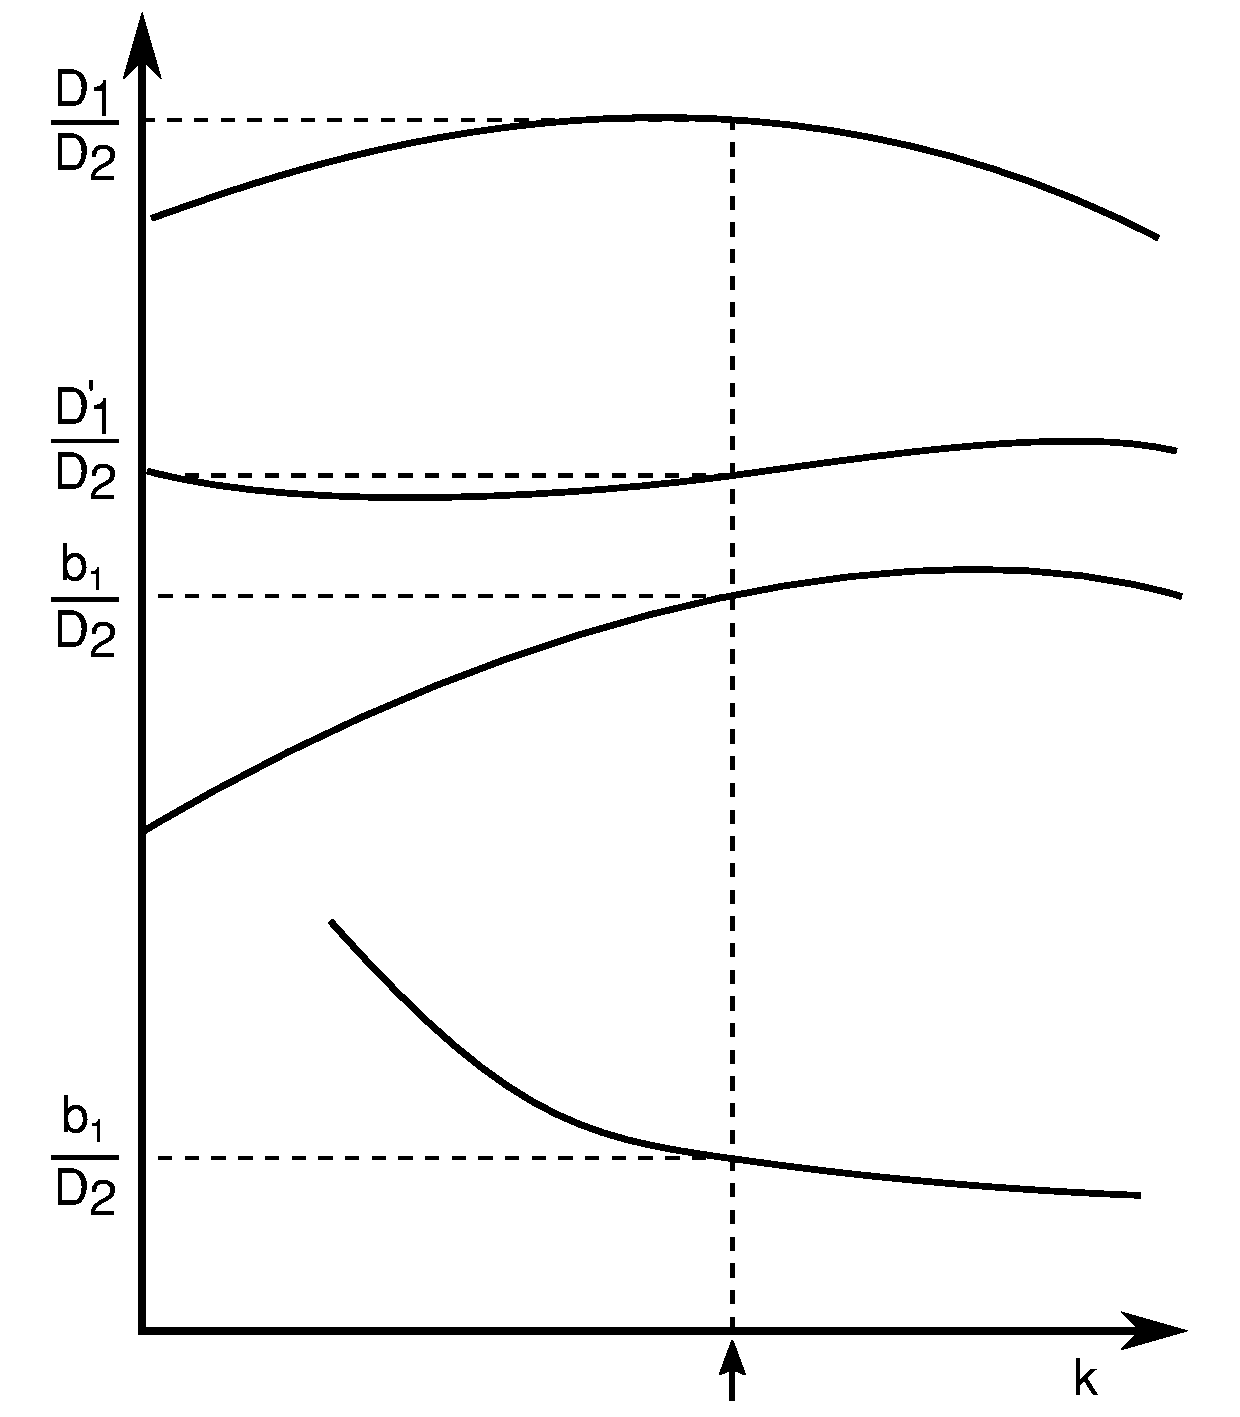
\includegraphics[width=.6\linewidth]{fig/primo_1.pdf}
  \captionof{figure}{}
  \label{fig:primo_1}
\end{minipage}
\end{figure}
Si definiscono le seguenti dimensioni caratteristiche più significative. Si tratta di un esempio didattico, in realtà posso andare a definire un database molto più ampio e raffinato. Siano
\begin{itemize}
\item[-]$D_2$: diametro massimo della girante;\\
\item[-]$D_1$: diametro massimo della sezione di ingresso;\\
\item[-]$D_1^{'}$: diametro minimo della sezione d'ingresso;\\
\item[-]$b_2$: altezza della pala in uscita;\\
\item[-]$b_1$: altezza della pala in ingresso.
\end{itemize}
Per definire $b_1$ bisogna prendere il diametro medio e con riferimento al punto di intersezione tra questo ed il profilo della pala in ingresso si traccia la circonferenza inscrivibile nella sezione d’ingresso. Come grandezza caratteristica della sezione d’ingresso prendo proprio il diametro di questa circonferenza.
Per queste grandezze posso definire le seguenti cifre adimensionali:
\begin{align*}
\frac{D_1}{D_2} \; \; \; \frac{D_1^{'}}{D_2} \; \; \; \frac{b_1}{D_2} \; \; \; \frac{b_2}{D_2} 
\end{align*}
Queste cifre sono funzioni di $k$. Posso allora essere definite delle curve che riportano in ascisse il valore del numero caratteristico $k$ ed in ordinate i valori dei 4 parametri.
Naturalmente fissato $k$ devo poi determinare il numero di giri a cui deve lavorare la macchina. 
Ricapitolando, note portata, prevalenza e fissata la velocità di rotazione, conosco il valore di $k$. Entrando in questi diagrammi si trovano i valori dei quattro parametri e quindi definisco per sommi capi la sezione meridiana della nostra macchina (figura \ref{fig:primo_1}).

Esiste una dimensione ottimale cioè una dimensione alla quale corrisponde il massimo rendimento. Bisogna però definire un’ulteriore grandezza detta diametro specifico.
\begin{equation}
D_s= \phi^{-1/2} \psi^{1/4} = D \cdot \frac{L_i^{1/4}}{\sqrt{Q}}
\end{equation}
Bisogna cercare di eliminare la velocità di rotazione. È stato verificato che esiste, con riferimento alle dimensioni di massimo rendimento, un legame tra $D_s$ e $w_s$. 
\begin{equation}
D_s=f(w_s)
\end{equation}
Questa funzione è descritta empiricamente sul \textit{Diagramma di Cordier}. Questo diagramma rappresenta l’interpolazione di una serie di dati sperimentali (da vedere come correlazione statistica).
Grazie alle curve di Balié è possibile osservare l’entità delle variazioni che si ottengono andando a discostarsi, entro certi limiti, dalla curva di Cordier.
Si può estendere questa relazione con i diagrammi di Baliè, intorno alla curva si disegnano curve di isorendimento.
\begin{figure}
\centering
\begin{minipage}{.5\textwidth}
  \centering
  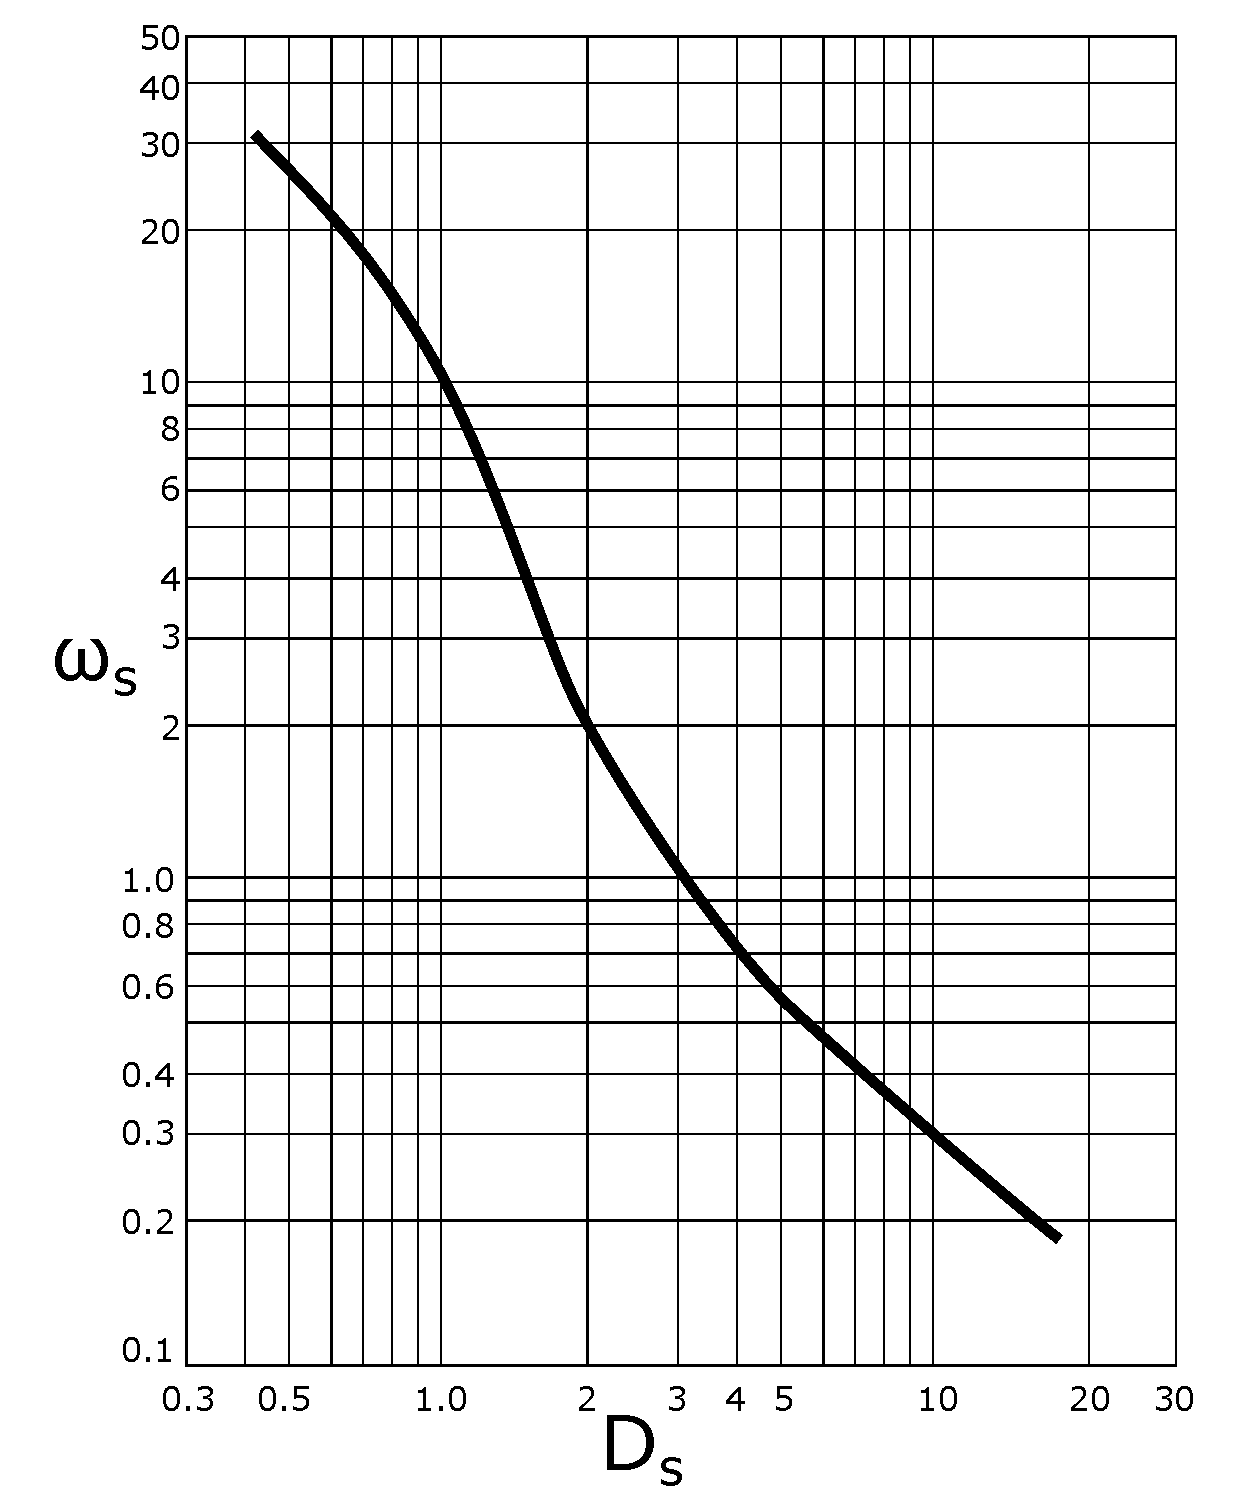
\includegraphics[width=.95\linewidth]{fig/cord_diag.pdf}
  \captionof{figure}{Diagramma di Cordier}
  \label{fig:cord_diag}
\end{minipage}%
\begin{minipage}{.5\textwidth}
  \centering
  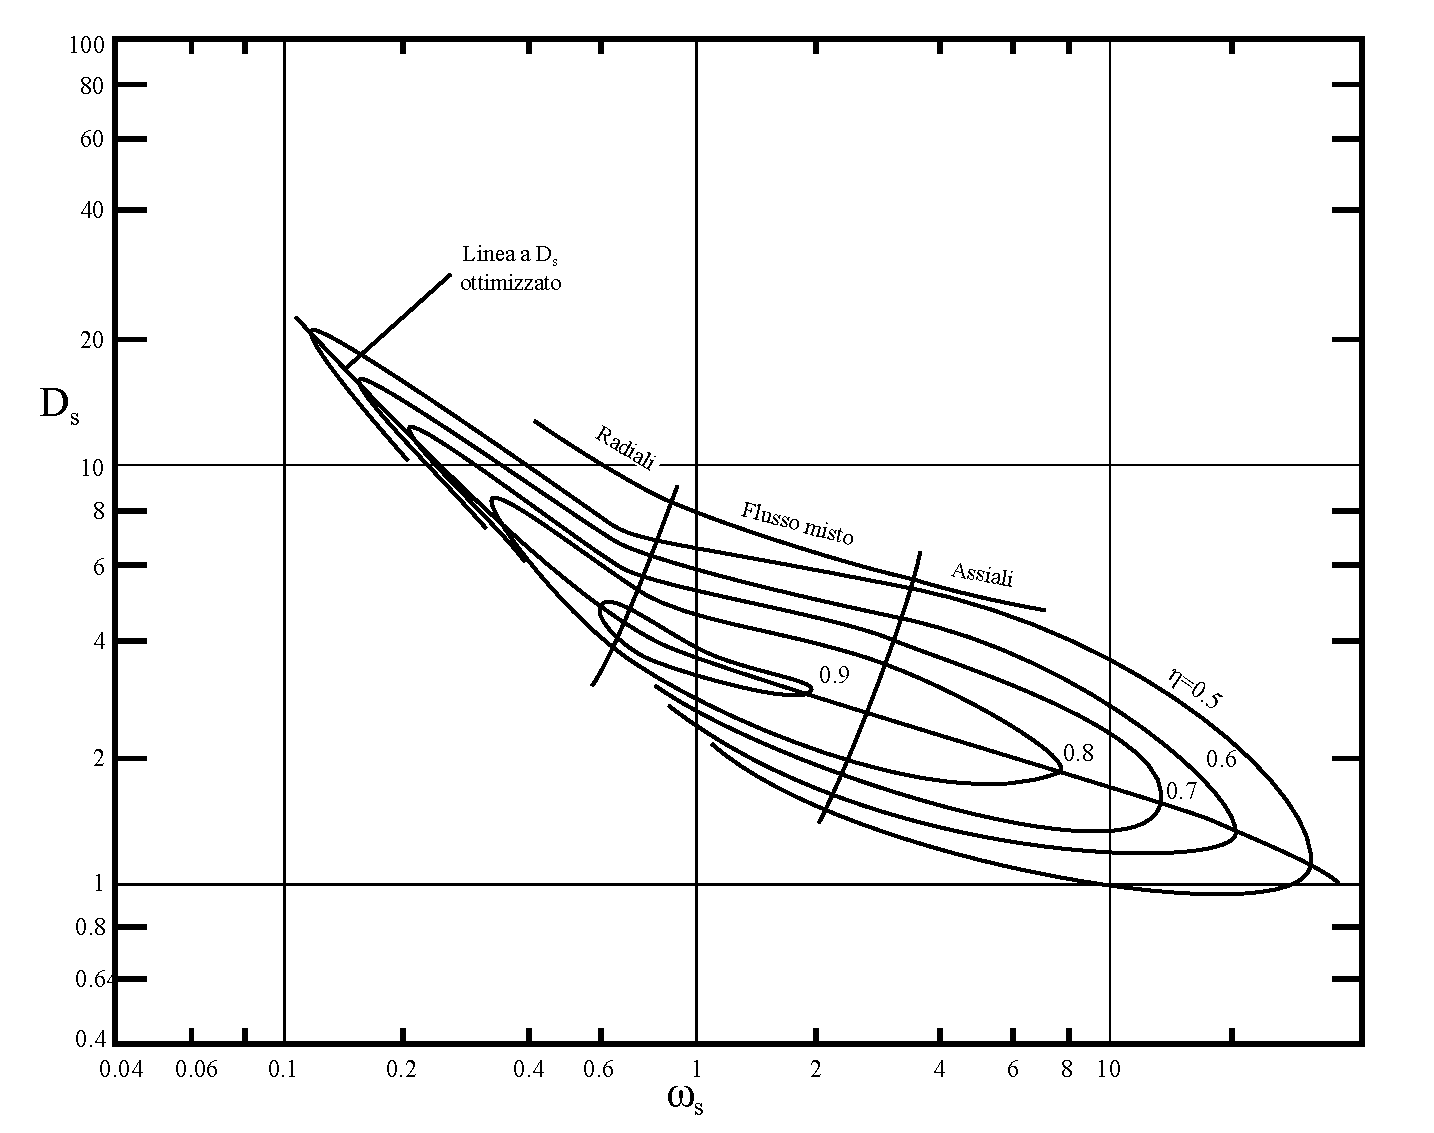
\includegraphics[width=.95\linewidth]{fig/primo_3.pdf}
  \captionof{figure}{}
  \label{fig:primo_3}
\end{minipage}
\end{figure}

\section{Influenza di Re}
Queste considerazioni sono state fatte trascurando l'influenza di Re. Ricordando il diagramma di Moody la relazione è fatta rispetto a $\epsilon/D$. Per le macchine è essenzialmente uguale, al diminuire di Re le curve si spostano più in basso, questo effetto si riflette in un abbassamento di rendimento e quindi di prevalenza.

Questo è un fenomeno prevedibile in termini statistici, storicamente grazie all'accumulazione di dati sono stati definiti due fattori di correzione, di rendimento $f_\eta$ e $f_\psi$ diagrammati ripsetto a $Re$. Man mano che $Re$ scende il loro effetto diventa sempre più importante. 
\begin{figure}
\centering
\begin{minipage}{.4\textwidth}
  \centering
  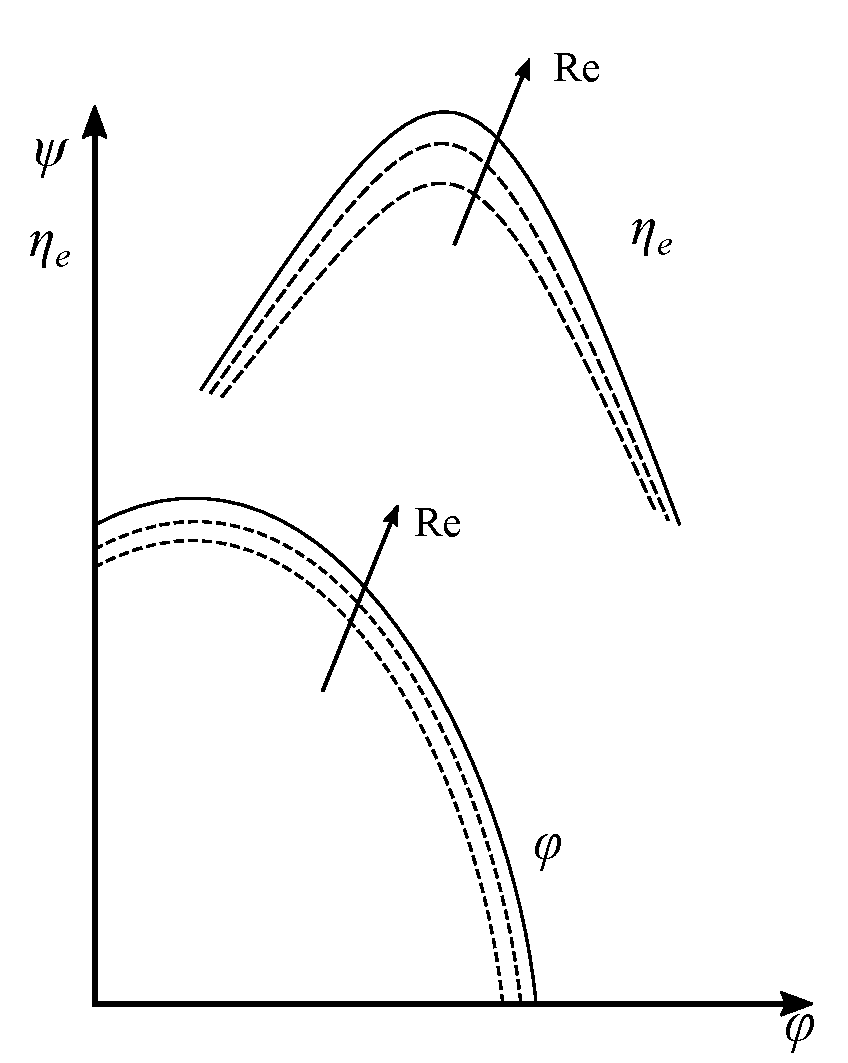
\includegraphics[width=.95\linewidth]{fig/secondo_1.pdf}
  \captionof{figure}{}
  \label{fig:secondo_1}
\end{minipage}%
\begin{minipage}{.6\textwidth}
  \centering
  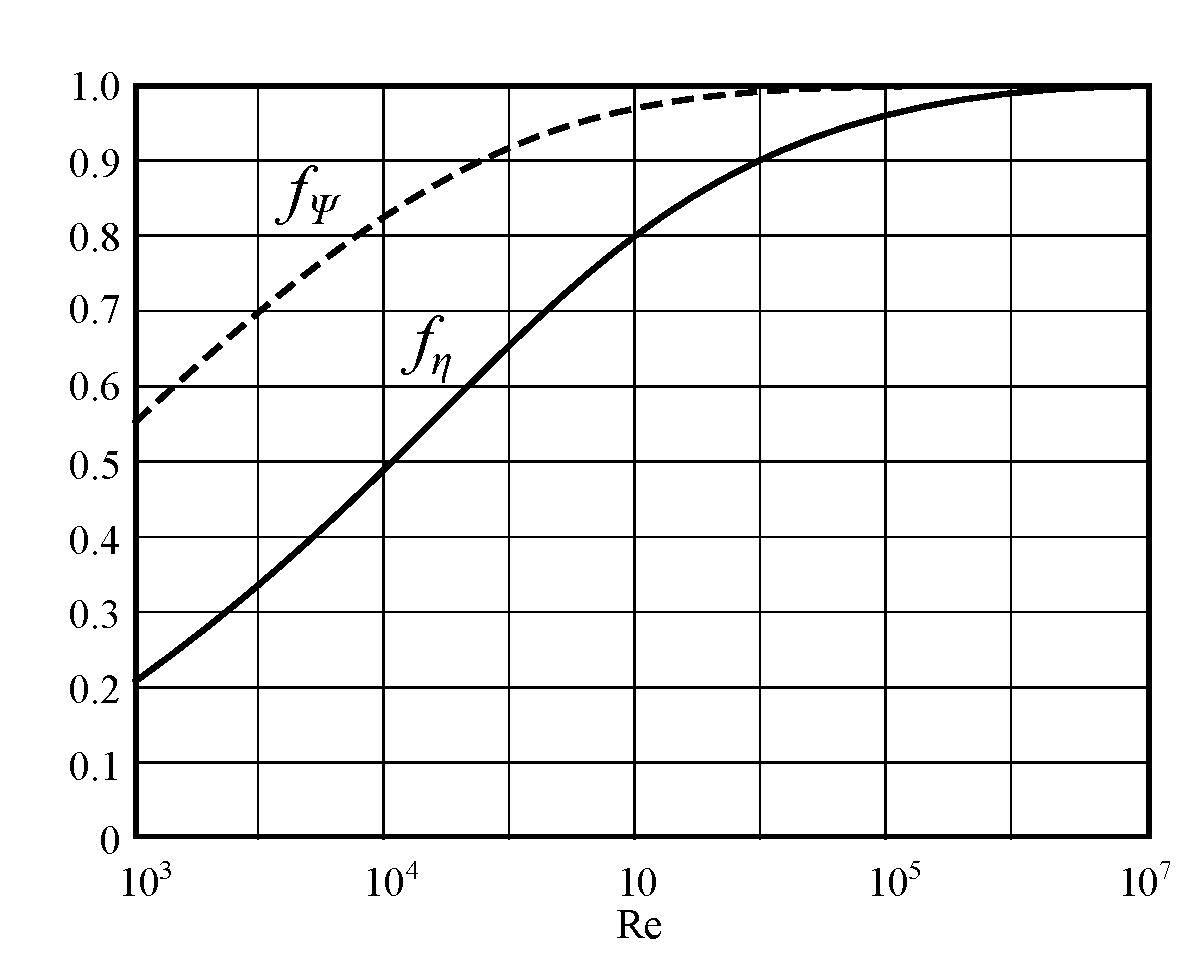
\includegraphics[width=.95\linewidth]{fig/secondo_2.pdf}
  \captionof{figure}{}
  \label{fig:secondo_2}
\end{minipage}
\end{figure}

Parto dalla $w_s$, scrivo $\Phi$ e $\psi$ nei diversi punti di funzionamento della macchina in funzione di $w_s$ ($\equiv k$). 
\begin{align*}
w_s= \phi^{1/2}\psi^{-3/4} \Rightarrow 
\begin{cases}
\psi = \psi(w_s)\\
\eta = \eta(w_s)
\end{cases}
\Rightarrow
\begin{cases}
f_{\psi} = f(Re)\\
f_{\eta} = f(Re)
\end{cases}
\end{align*}
Con i coefficienti correttivi vado a trovare le cifre adimensionali corrette \begin{align*}
\begin{cases}
\psi_{corretto} = f_{\psi} \cdot \psi(w_s)\\
\eta_{corretto} = f_{\eta} \cdot \eta(w_s)
\end{cases}
\end{align*}
A questo punto è possibile procedere a ritroso. Trovato il valore corretto avrò
\begin{align*}
\omega_s = \phi^{1/2} \psi^{-3/4} =  \phi_{corretto}^{1/2} \psi_{corretto}^{-3/4} = cost
\end{align*}
partendo proprio dalla definizione di $\omega_s$ è possibile costruire le curve di prestazione corrette.

\section{Effetto scala}
Si considera poi un effetto scala non solo legato alle rugosità superficiali ma anche legato ai giochi. L'effetto scala può essere espresso rispetto ai rapporti dimensionali. Queste relazioni sono sempre costruite per via empirica sulla base dei dati storici.

A parità di bontà di progettazione, geometria, ecc... la macchina grande ha un rendimento maggiore rispetto alla macchina piccola. Questo si spega facendo due osservazioni: a parità di tecnologia produttiva è possibile ritenere costante il valore della rugosità superficiale delle palettature della girante. In una macchina grande la rugosità relativa sarà quindi più bassa, quindi le perdite di carico saranno superiori nella macchina piccola. In secondo luogo bisogna tener conto dei giochi presenti tra parte fissa e parte mobile, che non possono scendere al di sotto di un certo limite. Nelle macchine grandi questi diventeranno trascurabili. 
\begin{figure}
\centering
  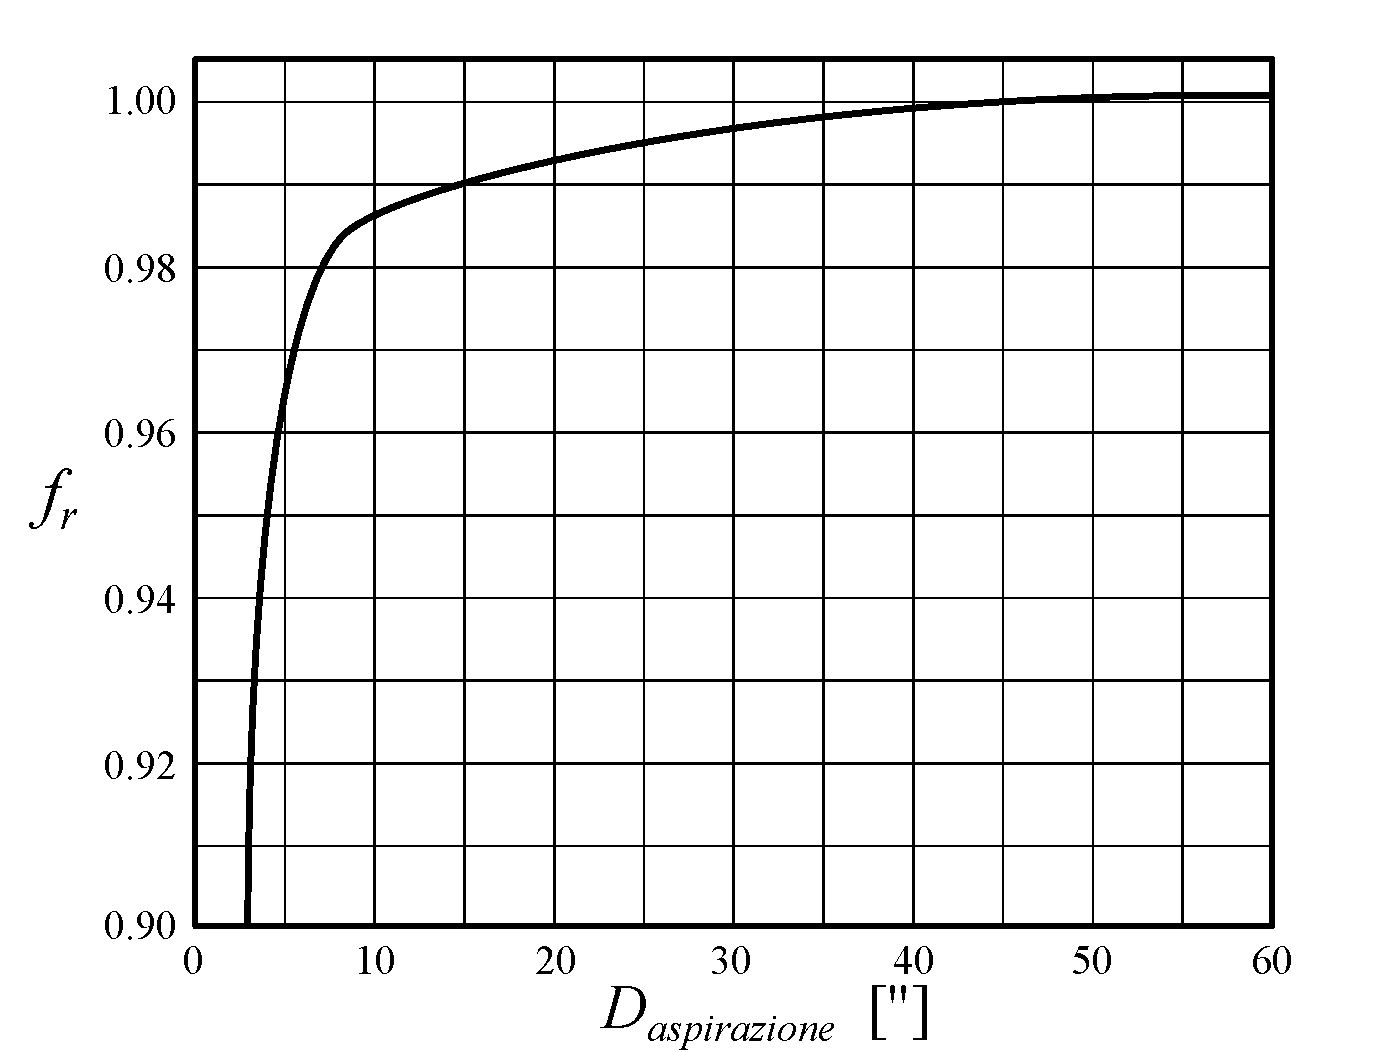
\includegraphics[width=.5\textwidth]{fig/dDchart.pdf}
\caption{}
\label{fig:dDchart}
\end{figure}

Facendo riferimento alle pompe possiamo definire un rapporto dimensionale 
\begin{align*}
\frac{D_1}{D_2} \triangleq  \mbox{Rapporto di scala}, \; D_1 < D_2
\end{align*}
In riferimento alla figura \ref{fig:dDchart} rendimento si può esprimere come
\begin{align*}
\eta = \eta_S \cdot f_r(D)
\end{align*}
E la relazione tra il rendimento tra le pompe di scala diversa è il seguente
\begin{equation}
\frac{1-\eta_1}{1-\eta_2} = \left( \frac{D_2}{D_1}\right)^\alpha
\end{equation}
La stessa operazione viene fatta per le turbine idrauliche
\begin{align*}
\frac{1-\eta_1}{1-\eta_2} = \left[ \frac{Re_{u,2}}{Re_{u,1}} \right]^n, \; \; n=0.1 \div 0.25
\end{align*}
\begin{align*}
\frac{1-\eta_1}{1-\eta_2} =0.5 + 0.5 \left[ \frac{Re_{u,2}}{Re_{u,1}} \right]^{0.2}
\end{align*}
\begin{align*}
\frac{1-\eta_1}{1-\eta_2} = 0.3 + 0.7 \left[ \frac{Re_{u,2}}{Re_{u,1}} \right]^{0.2} \; \to \; \mbox{Turbine Kaplan}
\end{align*}
\section{Flusso comprimibile}
Se si considera il flusso comprimibile le relazioni diventano più complesse. Infatti si ha:
\begin{equation}
\psi=f(\phi,Ma)
\end{equation}
$\psi$ dipende quindi anche dal numero di Mach. 
Nel diagramma $\phi-\psi$ si ottengono diverse curve al variare del numero di Mach (Figura \ref{fig:ComprMach}), le curve diventano di difficile lettura e comprensione.Infatti, per diversi valori delle grandezze termodinamiche di temperatura e pressione risulta possibile ottenere le stesse quantità di lavoro unitario, e ciò comporta una mancata definizione univoca dello stesso. Si tratta di una rappresentazione poco fisica e di un esercizio esclusivamente accademico.
\begin{figure}[h!]
\centering
  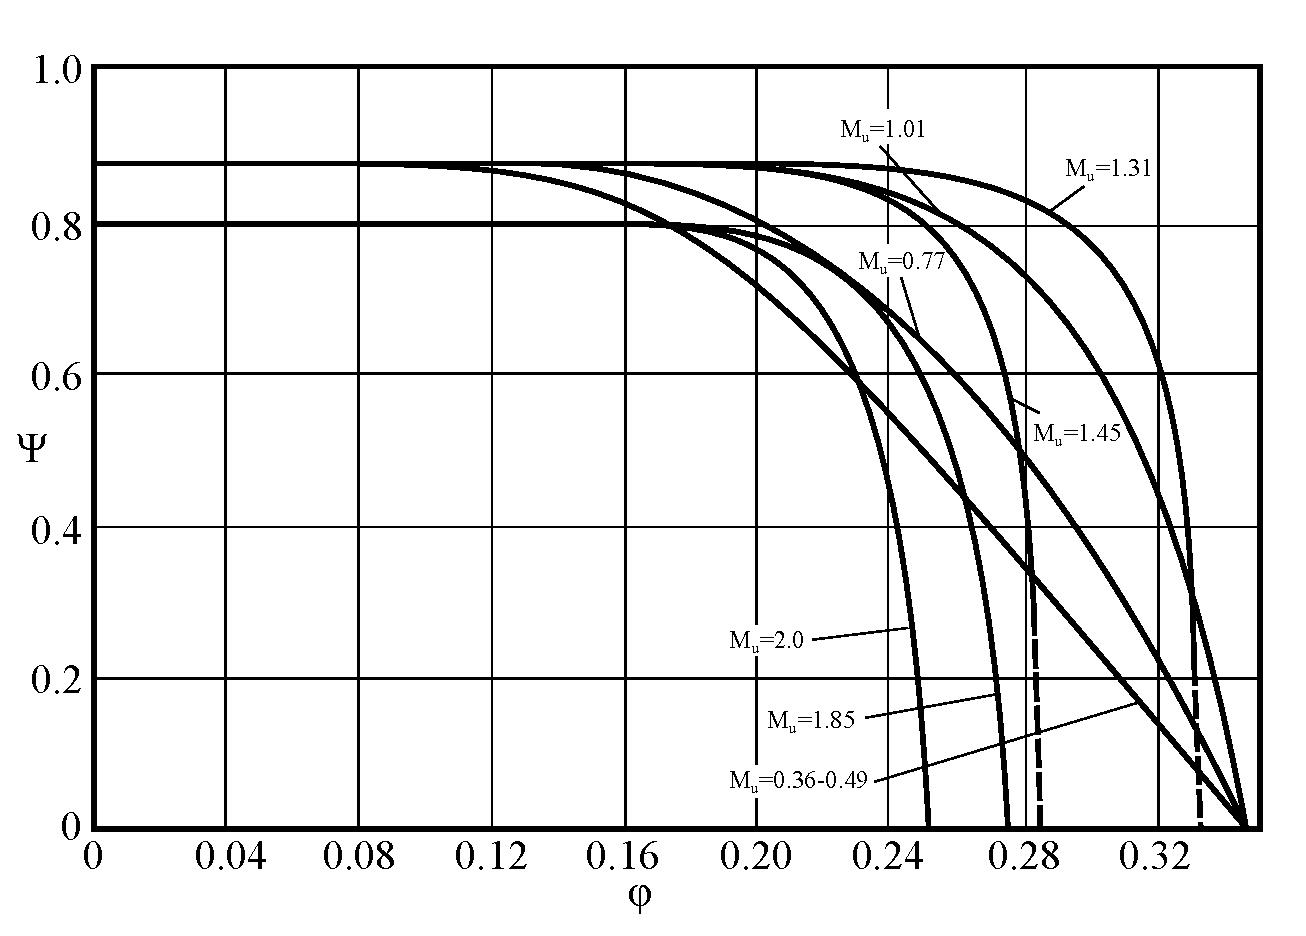
\includegraphics[width=.85\textwidth]{fig/ComprMach.pdf}
\caption{Curve adimensionali di funzionamento di una famiglia di compressori, per un fluido assegnato, a diversi numeri di Mach periferici. Sono definiti $Ma = \frac{w \frac{D}{2}}{a_{01}}$, $Mu = \frac{w \frac{D}{2}}{a}$}
\label{fig:ComprMach}
\end{figure}
Per questo tipo di macchine si utilizzaranno curve molto diverse. Per avere una grandezza confrontabile di funzionamento devo effettuare tutte le prove in condizioni standard. In questo modo posso rappresentare condizioni di funzionamento in modo univoco. 
Definisco il significato dei pedici:
\begin{itemize}
\item $s$: grandezze relative alle condizioni standard;
\item $c$: valori corretti, cioè riportati alle condizioni standard;
\item ``  ": valori da correggere rilevati nel corso della prova.
\end{itemize}
Si elencano di un gas generico miscela di due gas con massa molare $M$\footnote{Nota bene: solo in questo contesto si utilizza $M$ per indicare la massa molare, in tutto il resto del libro viene usato per indicare il numero di Mach}
\begin{align*}
\frac{p}{\rho} = \frac{p_1}{\rho} + \frac{p_2}{\rho} = x_1  \frac{p_1}{\rho_1} + x_2  \frac{p_2}{\rho_2} = RT \left( \frac{x_1}{M_1} + \frac{x_2}{M_2} \right) = RT(\frac{1}{M_{tot}})
\end{align*}
\begin{align*}
c_p = x_1 c_{p1} + x_2 c_{p2}
\end{align*}
\begin{align*}
\cfrac{\gamma}{\gamma -1} = \cfrac{\cfrac{x_1}{M_1} \cfrac{\gamma_1}{\gamma_1 -1}+\cfrac{x_2}{M_2} \cfrac{\gamma_2}{\gamma_2 -1}}{\cfrac{x_1}{M_1}+\cfrac{x_2}{M_2}}
\end{align*}
Con $M_{1,2,tot}$ numero di moli, $x_{1,2}$ frazione molare e $R$ costante dei gas perfetti. Si ricorda poi che definiti calore specifico a pressione costante $c_p$ e calore specifico a volume costante $c_v$ si ha
\begin{align*}
\gamma = \frac{c_p}{c_v}, \;\;\; R = c_p - c_v
\end{align*}

Di seguito venogono riportate le grandezze significative corrette rispetto alle condizioni standard.\\
Rapporto di compressione corretto rispetto alle condizioni ambientali standard:
\begin{align*}
\frac{p_{02}}{p_{01}} = \frac{p_{01c}}{p_{01s}} \; \Rightarrow \; p_{02c} = p_{02}\frac{p_{01s}}{p_{01}}
\end{align*}
Parametro di portata
\begin{align*}
\frac{\dot{m}\sqrt{T_{01}}}{p_{01}}=\frac{\dot{m_c}\sqrt{T_{01s}}}{p_{01s}} \; \Rightarrow \; \dot{m_c} = \dot{m} \sqrt{\frac{T_{01}}{T_{01s}}} \bigg(\frac{p_{01s}}{p_{01}} \bigg)
\end{align*}
Parametro di velocità
\begin{align*}
\frac{n}{\sqrt{T_{01}}}=\frac{n_c}{\sqrt{T_{01s}}} \; \Rightarrow \; n_c = n \sqrt{\frac{T_{01s}}{T_{01}}}
\end{align*}
Si definiscono quindi le condizioni ambientali standard.
Pressione ridotta
\begin{align*}
\delta = \frac{p_{01}}{p_{01s}}
\end{align*}
Temperatura ridotta
\begin{align*}
\theta = \frac{T_{01}}{T_{01s}}
\end{align*}
Si possono esprimere più sinteticamente le grandezze corrette:
\begin{align*}
p_{01c} = \frac{p_{02}}{\delta}
\end{align*}
\begin{align*}
\dot{m_c}= \dot{m} \frac{\sqrt{\theta}}{\delta}
\end{align*}
\begin{align*}
n_c = \frac{n}{\sqrt{\theta}}
\end{align*}
\begin{figure}
\centering
  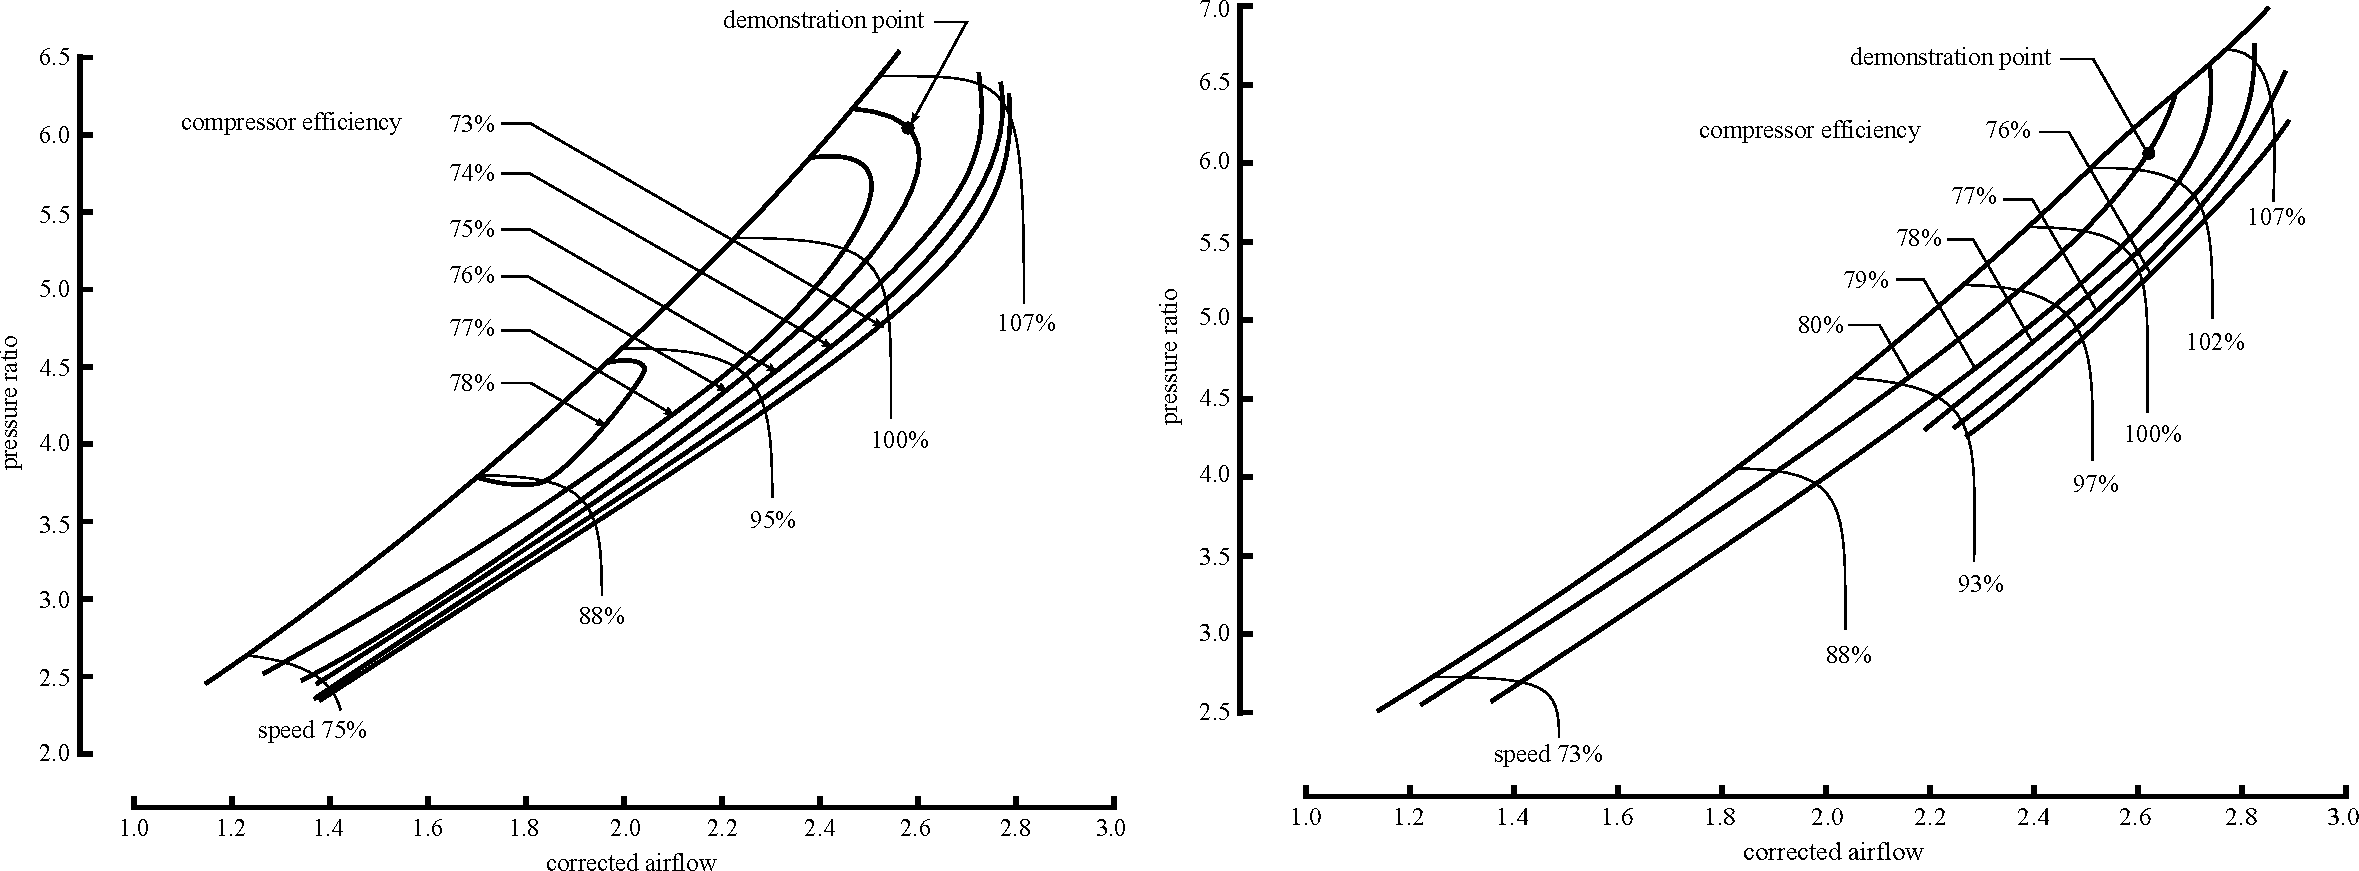
\includegraphics[width=\textwidth]{fig/CompMaps.pdf}
\caption{}
\label{}
\end{figure}
Si ottiene così la portata di massa corretta e il numero di giri corretto.
In questo modo si trovano le mappe di funzionamento delle macchine. Si diagrammano la portata d'aria corretta con il rapporto di compressione. Sono tracciate diverse curve al variare dei giri con le curve di isorendimento.

A questo punto si espande l'espressione di $\phi$ tenendo conto delle seguenti espressioni di $M_{01}$, $p$ e $a$
\begin{align*}
M_{01}=\frac{w D}{a_{01}}= \frac{w D}{\sqrt{k R T_{01}}}, \;\;\;p = \rho_i RT, \;\;\; a = \sqrt{k R T}
\end{align*}
\begin{equation}
\phi = \frac{\dot{m}}{\rho_{01} w D^3} = \frac{\dot{m}}{\rho_{01} M_{01} a_{01} D^2} = \frac{\dot{m} R T_{01}}{\rho_{01} M_{01} \sqrt{k R T_{01}} D^2} = \frac{\dot{m} \sqrt{R T_{01}}}{\rho_{01} M_{01} \sqrt{k} D^2}
\end{equation}
Mentre la cifra $\psi$ è esprimibile in funzione dei soli $M_{01}$, rapporto di compressione e delle caratteristiche del fluido ($k$)
\begin{equation}
\psi = \cfrac{L_i}{w^2 D^2} = \cfrac{\Delta h_{0s}}{w^ 2 D^2} = \cfrac{\cfrac{k}{k-1} R T_{01}\left[ \bigg( \cfrac{p_{02}}{p_{01}} \bigg)^{\frac{k-1}{k}}-1\right]}{M_{01}^2 k R T_{01}} = \cfrac{\cfrac{1}{k-1} \left[ \bigg( \cfrac{p_{02}}{p_{01}} \bigg)^{\frac{k-1}{k}}-1\right]}{M_{01}^2 }
\end{equation}

L'idea è quella di rappresentare in modo univoco il comportamento del compressore usando i termini $\phi$, $\psi$ ma mantenendo la significatività fisica.

Se utilizzo lo stesso fluido posso trascurare $R$ e $k$. Utilizzando la stessa macchina trascuro anche $D$, riferendosi alle condizioni standard posso considerare $M_{01}=cost$. Sotto le precedenti ipotesi ottengo le seguenti relazioni semplificate:
\begin{align*}
M_{01} \to \frac{w D}{\sqrt{R T_{01}}} \Rightarrow M_{01} \to \frac{w}{\sqrt{T_{01}}}
\end{align*}
\begin{align*}
\phi \to \frac{\dot{m} \sqrt{RT_{01}}}{\rho_{01} D^2} \Rightarrow \phi \to \frac{\dot{m} \sqrt{T_{01}}}{\rho_{01}}
\end{align*}
\begin{align*}
\psi \to \frac{p_{02}}{p_{01}}
\end{align*}
Si tratta di grandezze che posso andare a misurare in un banco prova. 
La mappa di funzionamento del compressore assume quindi una forma più leggibile, sull'asse delle ascisse ho la portata in massa corretta con la temperatura in ingresso e sulle ordinate il rapporto di compressione. Assieme a queste posso anche costruire le linee di isorendimento  e quindi la curva ideale operativa del compressore data dall'inviluppo delle curve di isorendimento.
\begin{figure}
\centering
  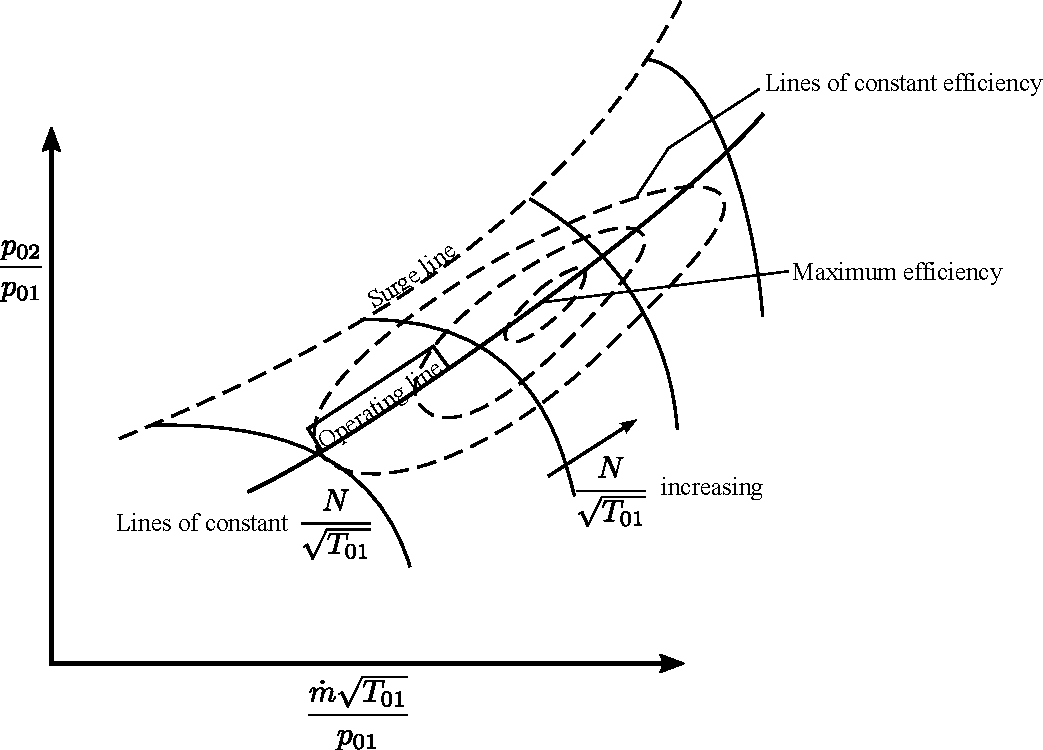
\includegraphics[width=.8\textwidth]{fig/secondo_8.pdf}
\caption{}
\label{fig:secondo_8}
\end{figure}
Guardando al diagramma in figura \ref{fig:secondo_8} si vede che abbiamo un fenomeno noto come ingolfamento del compressore, in particolare si vede dalle linee a velocità costante che tendono a diventare verticali in prossimità dele condizioni di ingolfamento . Intendiamo il raggiungimento di quella condizione di funzionamento in cui non è più possibile variare la portata variando il rapporto delle pressioni attorno alla macchina.
Questo perchè in qualche punto si raggiungono le condizioni di flusso sonico e quindi, ricordando lo studio dell’ugello convergente-divergente, abbiamo un
blocco sonico delle portata.

L'obiettivo è quello di lavorare il più possibile vicino alla ``operating line" che è la zona di massimo rendimento, il problema è che ci si trova pericolosamente vicino alla ``surge line". Oltre la surge line si innesca il fenomeno del pompaggio che può compromettere la macchina e l'impianto irrimediabilmente.

Riassumendo, nel comprimibile, operativamente si descrive il funzionamento delle turbomacchine non rispetto alle cifre di flusso e pressione, bensì attraverso nuove cifre più significative in questo contesto.
\section{Richiamo di termodinamica}
Lo scambio termico è trascurabile per i bassi tempi di residenza del fluido nel condotto.

Rotore adiabatico
\begin{equation}
L_{12}^{'} = h_{t1}-h_{t2}
\end{equation}
\begin{equation}
h_t=h+\frac{c^2}{2}+gz
\end{equation}
\begin{equation}
L_{12}^{'} = \begin{cases} u_1 c_{u1}-u_2 c_{u2}\\
\cfrac{c_1^2-c_2^2}{2}+\cfrac{u_1^2-u_2^2}{2}-\cfrac{w_1^2-w^2}{2} \end{cases}
\end{equation}

Naturalmente il lavoro è stato scritto, in base alle note convenzioni, per una macchina motrice.

Il lavoro è composto da una parte cinetica ($c$) e da una parte statica ($u,w$). 

Risulta chiaro che una macchina radiale avrà anche le componenti statiche, a differenza di una macchina puramente assiale, potra quindi, a parità di stadi, eseguire un maggior lavoro.

Ponendomi come osservatore relativo rispetto al rotore posso scrivere
\begin{equation}
u_1 c_{u1} - u_2 c_{u2} = h_1 + \frac{c_1^2}{2}+gz_1-h_2-\frac{c_2^2}{2}-gz_2
\end{equation}
Posso quindi definire la rotalpia come grandezza di stato:
\begin{equation}
h+\frac{c^2}{2}+gz-u c_u = cost. = I
\end{equation}

Riassumento:
\begin{itemize}
\item $I=cost.$ in un rotore adiabatico;
\item $h_t=cost.$ in uno statore adiabatico.
\end{itemize}

Posso esprimere tutte le grandezze fin'ora viste in un piano $T-s$ o $h-s$.

I rendimenti sono da sbobinare.
\pagebreak

\chapter{Turbine a flusso assiale e misto}
Nel caso delle turbine non si parlerà di flusso assiale puro, è presente anche una significativa componente radiale. Nel caso di una turbina il salto entalpico per stadio è di gran lunga superiore all'analogo elaborabile dal compressore. Entalpia e temperatura decrescono molto rapidamente, l'ipotesi di avere densità costante e l'andamento delle pressioni a gradino tra stadi successivi non è più accettabile a causa proprio della dimensione del salto entalpico. Abbiamo temperature molto elevate, nel compressore è la qualità del design del profilo a dominare mentre nella turbina il limite costruttivo è dato dai materiali della palettatura che lavorano a temperature molto elevate e con deflessioni che vanno dai $50^{\circ} a 180^{\circ}$. 
\begin{figure}[h!]
\centering
  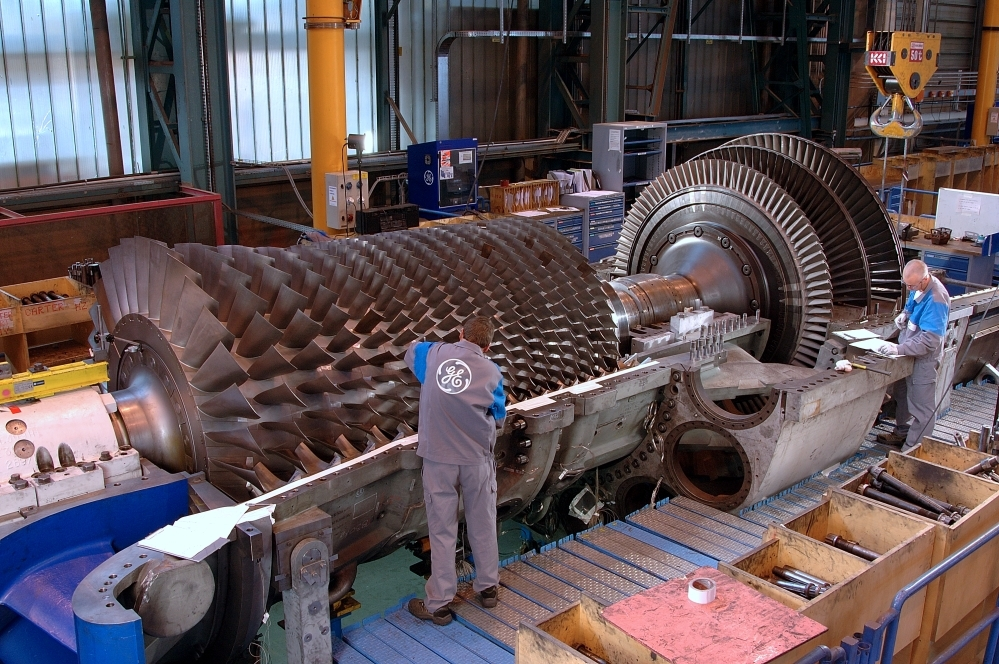
\includegraphics[width=.9\textwidth]{fig/TurboGas.png}
\caption{}
\label{fig:TurboGas}
\end{figure}
Il proilo aerodinamico utilizzato in un compressore sarà quindi molto diverso da quello utilizzato in una turbina, quest'ultimo rappresenta più una effettiva variazione di condotto. 
Per andare a vedere come si presenta una turbina assiale facciamo riferimento all'immagine in figura \ref{fig:TurboGas}, è rappresentata una turbina a gas ad uso terrestre. Le pale sono attorno ai 45 gradi, immaginando la parte statorica si avrà un grado di reazione di 0.5, probabilmente ad eccezione del primo stadio, a monte potrebbe esserci un IGV. Sono presenti $17$ stadi di compressione e solo $3$ di turbina. 

Vediamo allora quali possono essere le varie configurazioni di turbina. 
Vi sono innanzitutto gli stadi ad azione $R = 0$
\begin{align*}
\begin{cases}
\mbox{De laval}, & z_v = 1\\
\mbox{Curtis}, & z_v = 2 \div 3\\
\mbox{Reteau}, & z_v = 1\\
\end{cases}
\end{align*}
Con $z_v$ salti di velocità. Ci sono poi le turbine Parsons con $R = 5$. Si possono così andare a determinare i triangoli di velocità.

\begin{align*}
\bigg( \frac{u}{c_1} \bigg)_{opt} = \frac{\sin \alpha_1}{2 z_v}, \; \mbox{per} \; R = 0
\end{align*}
\begin{align*}
\bigg( \frac{u}{c_1} \bigg)_{opt} = \sin \alpha_1, \; \mbox{per} \; R = 0.5
\end{align*}
Poi essento $\alpha_1$ piccolo si può scrivere $ \sin \alpha_1 \simeq \alpha_1$ semplificando ulteriormente le espressioni.

\section{Calcolo dei rendimenti}
Andiamo ora a vedere quello che succede all'interno dello stadio di una turbina. Mi pongo su un sistema di riferimento con linea media del condotto palare come mostrato in \ref{fig:SezioneTurbina}. Non posso più assumere trascurabile la variazione di raggio. 
\begin{figure}
\centering
\begin{minipage}{.5\textwidth}
  \centering
  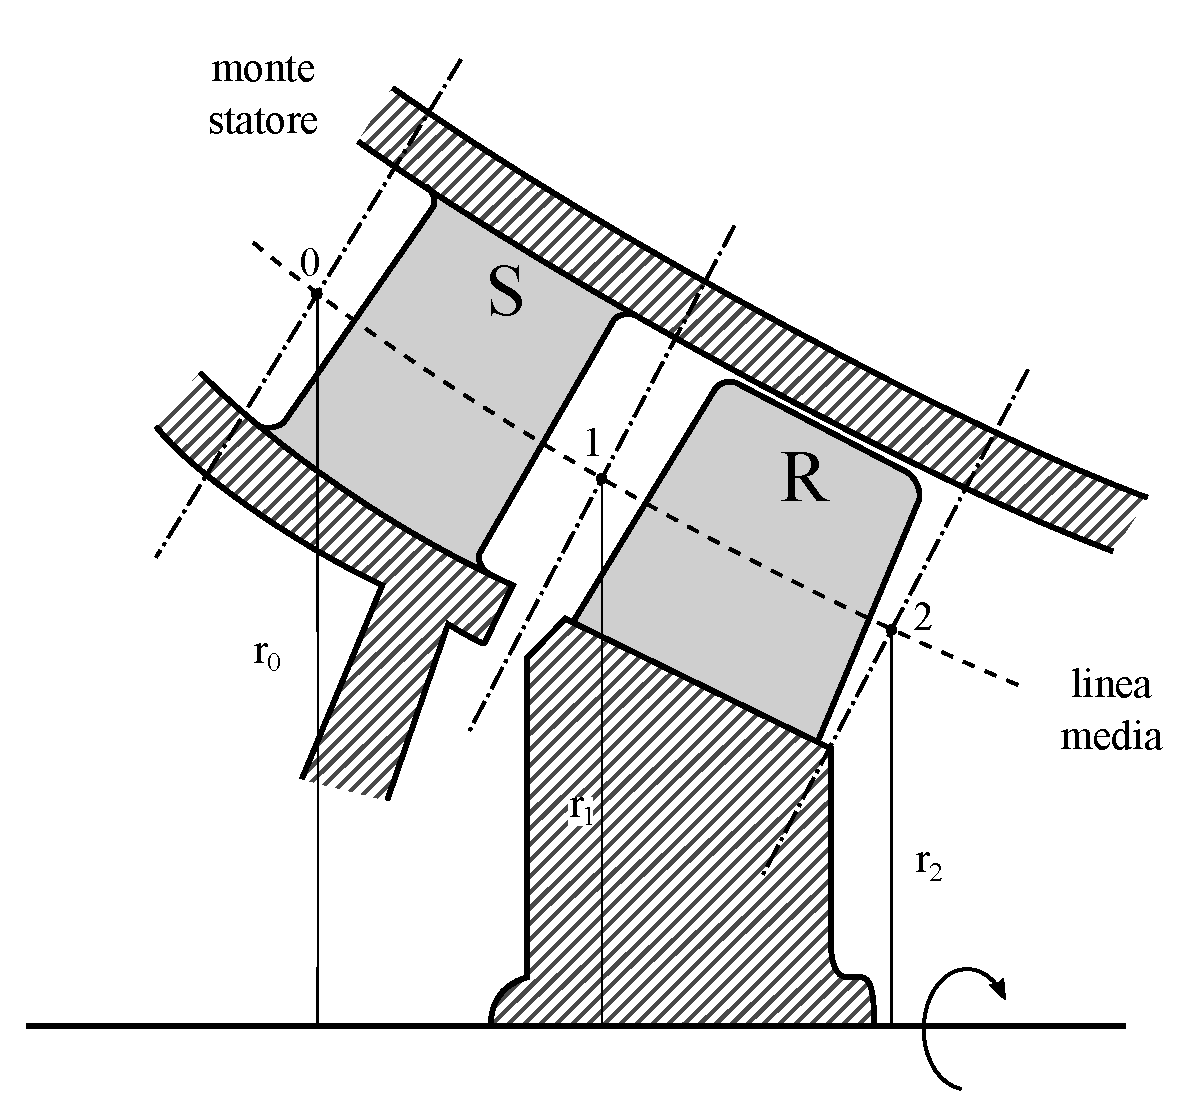
\includegraphics[width=.95\linewidth]{fig/SezioneTurbina.pdf}
  \captionof{figure}{}
  \label{fig:SezioneTurbina}
\end{minipage}%
\begin{minipage}{.5\textwidth}
  \centering
  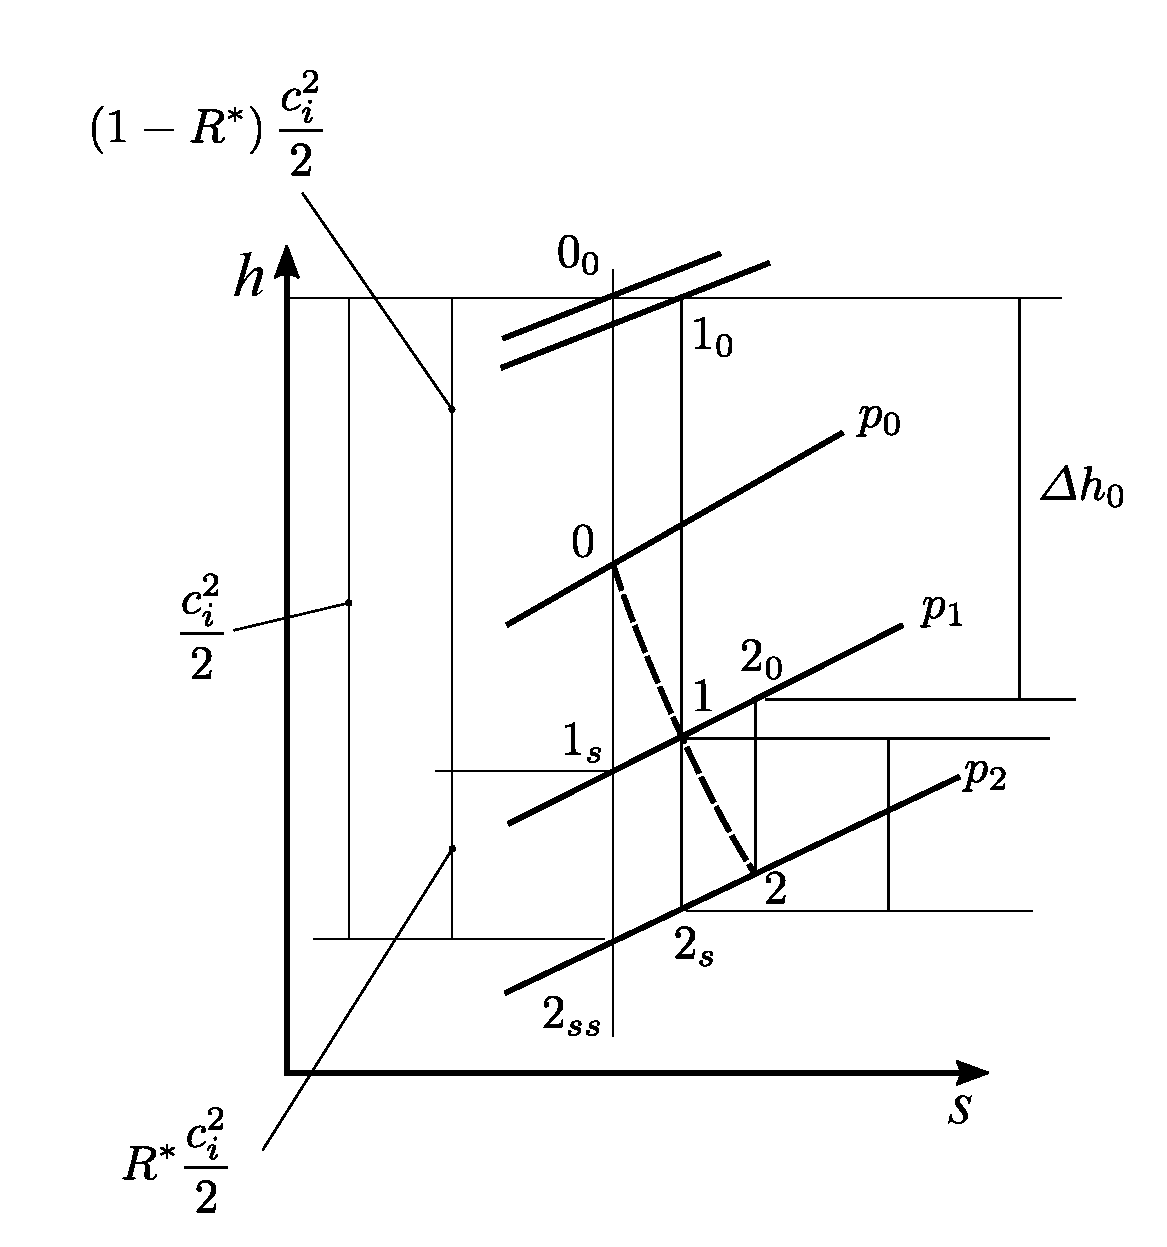
\includegraphics[width=.95\linewidth]{fig/hsturbine.pdf}
  \captionof{figure}{}
  \label{fig:hsturbine}
\end{minipage}
\end{figure}
Il salto entalpico tra i punti $1 - 2_s$ è leggermente superiore a quello presente tra i punti $1_s - 2_{ss}$ questo a causa della divergenza delle isobare. A tal proposito si introduce il fattore di recupero $f$ 
\begin{align*}
(1- R^*) \cdot \frac{c_i^2}{2}
\end{align*}
\begin{align*}
(1+f)r^* \cdot \frac{c_i^2}{2} \; \mbox{salto tra $1$ e $2_s$}
\end{align*}
Questo fattore di recupero è fisicamente spiegabile dal fatto che la trasformazione non essendo puramente isoentropica causa un aumento della temperatura parzialmente recuperabile nell'attraversamento successivo. 

\subsection{Rendimenti}
Il rendimento è il seguente
\begin{align*}
\eta = \cfrac{h_{0_0} - h_{0_2}}{h_{0_0} - h_{2_{ss}} - \Phi_E \cfrac{c_2^2}{2}} = \frac{\Delta h_0}{\Delta h_{is_{ts}}-\Phi_E \cfrac{c_2^2}{2}}
\end{align*}
Il termine fi e rappresenta la quota cinetica a valle della turbina. Quando lo considero uguale a 1 sto considerando un rendimento total to total mentre se lo considero pari a zero sto considerando un rendimento total to static.
\begin{align*}
\begin{cases}
\Phi_E = 1 \; \Rightarrow & \eta = \eta_{tt}\\
\Phi_E = 0 \; \Rightarrow & \eta = \eta_{ts}
\end{cases} 
\end{align*}
Seguono ora una serie di definizioni. Cifra di lavoro
\begin{align*}
\psi = \cfrac{h_{0_0} - h_{2_{ss}}}{\cfrac{u^2}{2}} = \frac{c_1^2}{u_1^2} = \frac{\Delta h_{is_{ts}}}{\cfrac{u^2}{2}}
\end{align*}
Coeiciente di portata
\begin{align*}
\Phi_1 = \frac{c_{m1}}{u_1}
\end{align*}
Grado di reazione
\begin{align*}
R^* = \frac{h_{1s} - h_{2ss}}{h_{0_0} - h_{2_{ss}}} = \frac{\Delta h_{Ris}}{\Delta h_{ists}}
\end{align*}
Energia cinetica totale
\begin{align*}
\frac{c_i^2}{h_{0_0} - h_{2_{ss}}}
\end{align*}
Coeiciente di velocità periferica
\begin{align*}
k_{is} = \frac{u_1}{c_1} = \frac{1}{\sqrt{\psi}}
\end{align*}
Coefficiente di lavoro specifico totale
\begin{align*}
\lambda = \cfrac{h_{0_0} - h_{2_0}}{\cfrac{u^2}{2}} \frac{\Delta h_0}{\frac{u^2}{2}}
\end{align*}
Voglio cercare la relazione tra il grado di reazione ideale e quello effettivo. Adimensionalizzo i triangoli di velocità. Ora non posso più riferirmi ad una sola velocità meridiana, questa diventa una grandezza di progettazione in quanto definisce le sezioni della macchina. Utilizzo quindi i rapporti tra velocità meridiane e tra i raggi.
\begin{align*}
\frac{c_{m2}}{c_{m1}}, \;\; \frac{r_2}{r_1}
\end{align*}
Adimensionalizzo tutte le grandezze con la velocità periferica $u_1$. Chiaramente i triangoli di velocità saranno di dimensioni diverse. 
\begin{figure}[h!]
\centering
  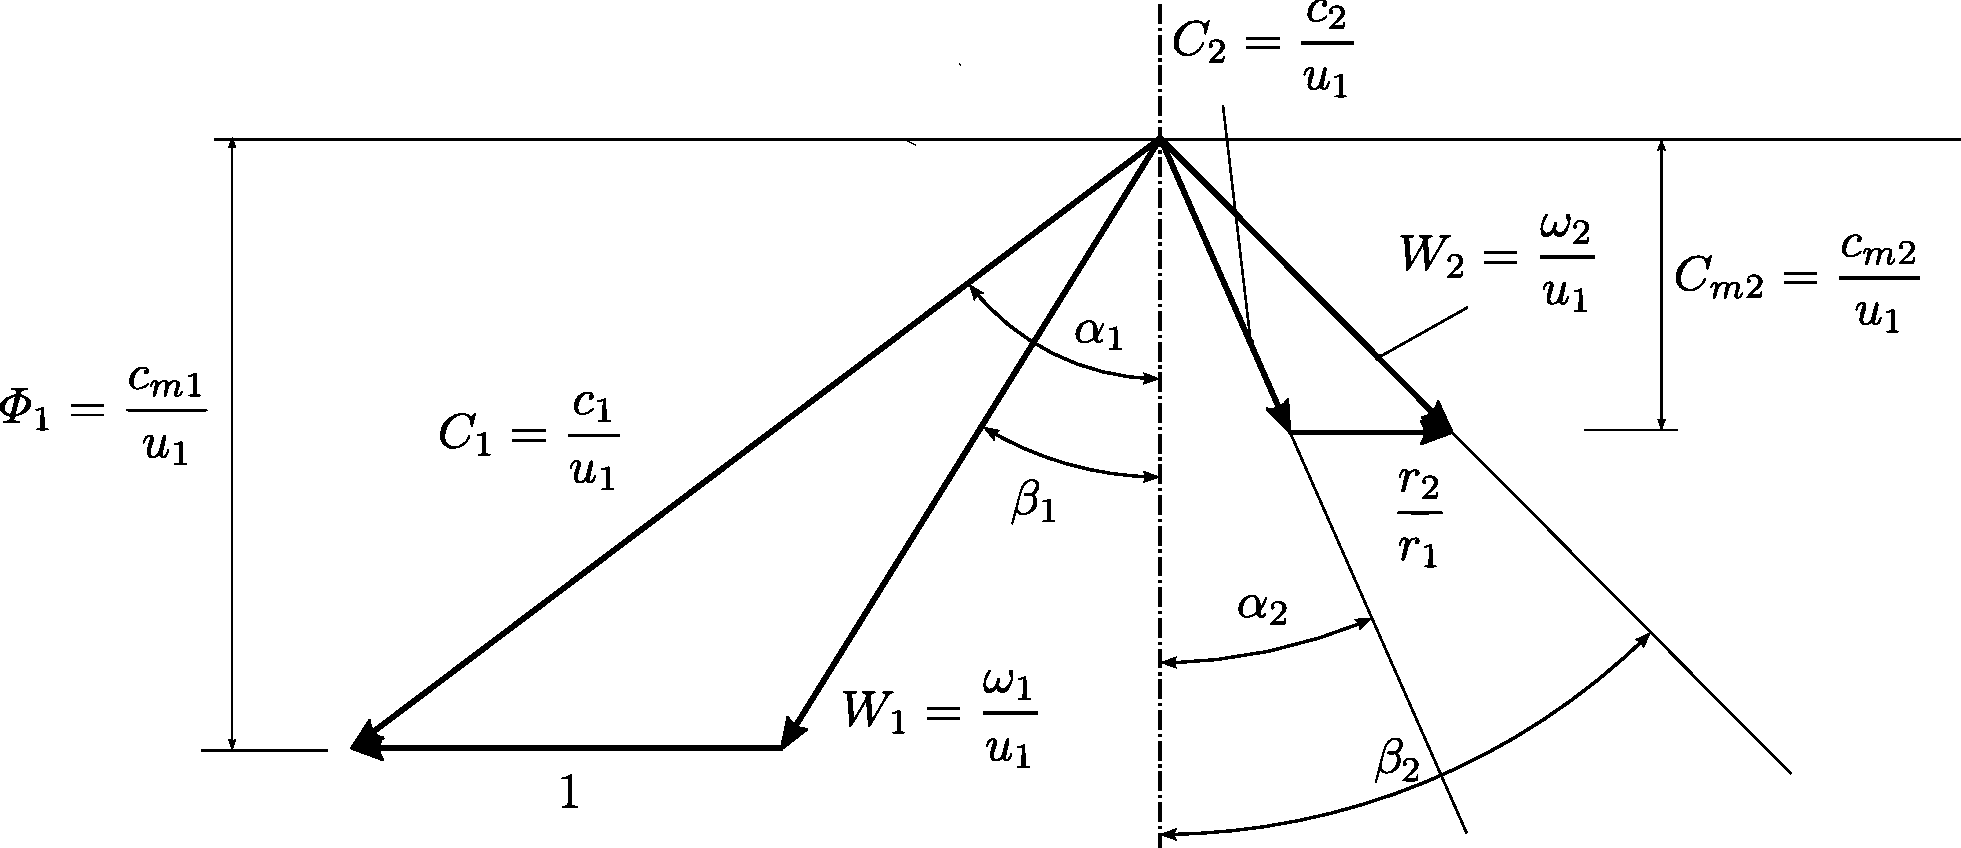
\includegraphics[width=.8\textwidth]{fig/triangTurb.pdf}
\caption{}
\label{fig:triangTurb}
\end{figure}
Posso ora andare a sviluppare l'espressione del rendimento
\begin{equation}
\eta = \cfrac{\Delta h_0}{\Delta h_{is_{ts}} - \Phi_E \cfrac{c_2^2}{2}} \cdot \frac{\frac{1}{u_1^2/2}}{\frac{1}{u_1^2/2}} = \frac{\lambda}{\psi - \Phi_E \left( C_2^2 \right)}
\end{equation}
Espandendo il numeratore
\begin{align*}
\lambda = \cfrac{\Delta h_0}{\cfrac{u_1^2}{2}} = \frac{2 \left( u_1 c_{u1} - u_2 c_{u2} \right)}{u_1^2} = 2 \bigg( C_{u1} - \frac{r_2}{r_1} C_{u2} \bigg)
\end{align*}
Scrivo ora le velocità assolute adimensionalizzate in funzione del rendimento e del grado di reazione. 
\begin{align*}
\frac{c_1^2}{2} = \left( 1 - R^* \right) \frac{c_i^2}{2} \cdot \eta_s \; \Rightarrow \; c_1 = \sqrt{\eta_s \left( 1 - R^* \right)} \cdot c_i
\end{align*}
\begin{align*}
C_1 = \frac{c_1}{u_1} = \sqrt{\eta_s \left(1- R^* \right)} \cdot \frac{c_i}{u_1}, \; \mbox{con } \frac{c_i}{u_1} = \frac{1}{k_{is}}
\end{align*}
Ottengo
\begin{equation}
\boxed{ C_1 = \frac{\sqrt{\eta_s}}{k_{is}} \sqrt{1 - R^*} }
\end{equation}
Vado a vedere la stessa cosa per le altre grandezze. Per espandere la velocità relativa adimensionalizzata utilizzo il teorema di Carnot
\begin{align*}
W_1^2 = C_1^2 + 1^2 - 2 \cdot 1 \cdot C_1 \cos \big( \frac{\pi}{2} - \alpha_1 \big)
\end{align*}
ottengo
\begin{align*}
\boxed{ W_1 = \sqrt{1 + \frac{n_{is}}{k_{is}^2} \left( 1 - R^* \right) - 2 \frac{\sqrt{\eta_s}}{k_{is}} \sqrt{1-R^*} \cdot \sin \alpha_1}}
\end{align*}
Per quanto riguarda $W_2$. Considero il salto entalpico e lo scrivo in funzione del fattore di recupero
\begin{equation}
h_2 - h_1 = \frac{u_2^2 - u_1^2}{2} - \frac{\omega_2^2 - \omega_1^2}{2}
\end{equation}
\begin{align*}
h_1 - h_2 = \frac{c_i^2}{2} \cdot R^* \left( 1 + f \right) \eta_R
\end{align*}
\begin{align*}
\left. \frac{\omega_2^2 - \omega_1^2}{2} - \frac{u_2^2 - u_1^2}{2} = \frac{c_i^2}{2} \cdot R^* \left( 1 + f \right) \eta_R \; \; \cdot \middle/ \frac{1}{u_1^2} \right.
\end{align*}
\begin{equation}
\boxed{W_2 = \sqrt{\frac{\eta_R \left( 1 + f \right) R^*}{k_{is}^2} + \frac{\eta_s}{k_{is}^2}  \left(1 + R^* \right) - \frac{2 \sqrt{\eta_s}}{k_{is}} \sqrt{1 - R^*} \sin \alpha_1 + \bigg(\frac{r_2}{r_1} \bigg)^2 } }
\end{equation}

Per quanto riguarda $C_{m2}$ 
\begin{align*}
c_{m2} = c_{m1} \frac{c_{m2}}{c_{m1}} c_1 \cos \alpha_1 \cdot \frac{c_{m2}}{c_{m1}}
\end{align*}
\begin{align*}
C_{m2} = C_1 \cos \alpha_1 \cdot \frac{c_{m2}}{c_{m1}}
\end{align*}
ottengo
\begin{equation}
\boxed{C_{m2} = \frac{c_{m2}}{c_{m1}} \frac{\sqrt{\eta_s}}{k_{is}} \sqrt{1 - R^*} \cos \alpha_1 }
\end{equation}
Sono in grado essenzialmente di scrivere il rendimento come funzionale di tutte le grandezze viste 
\begin{align*}
\eta = f \bigg( \psi, \Phi_R, R^*, k_{is}, f, \frac{c_{m2}}{c_{m1}}, \frac{r_2}{r_1}, \alpha_1, \eta_s, \eta_R \bigg)
\end{align*}
I primi quattro parametri sono parametri unzionali, $f$ dipende dalla divergenza delle isobare e quindi dalla natura del fluido, i tre parametri successivi sono parametri di progetto e infine gli ultimi due sono parametri della schiera rotorica e statorica.
Possiamo tracciare un diagramma di rendimento total - static / total - total in funzione della cifra di lavoro. 
\begin{figure}
\centering
  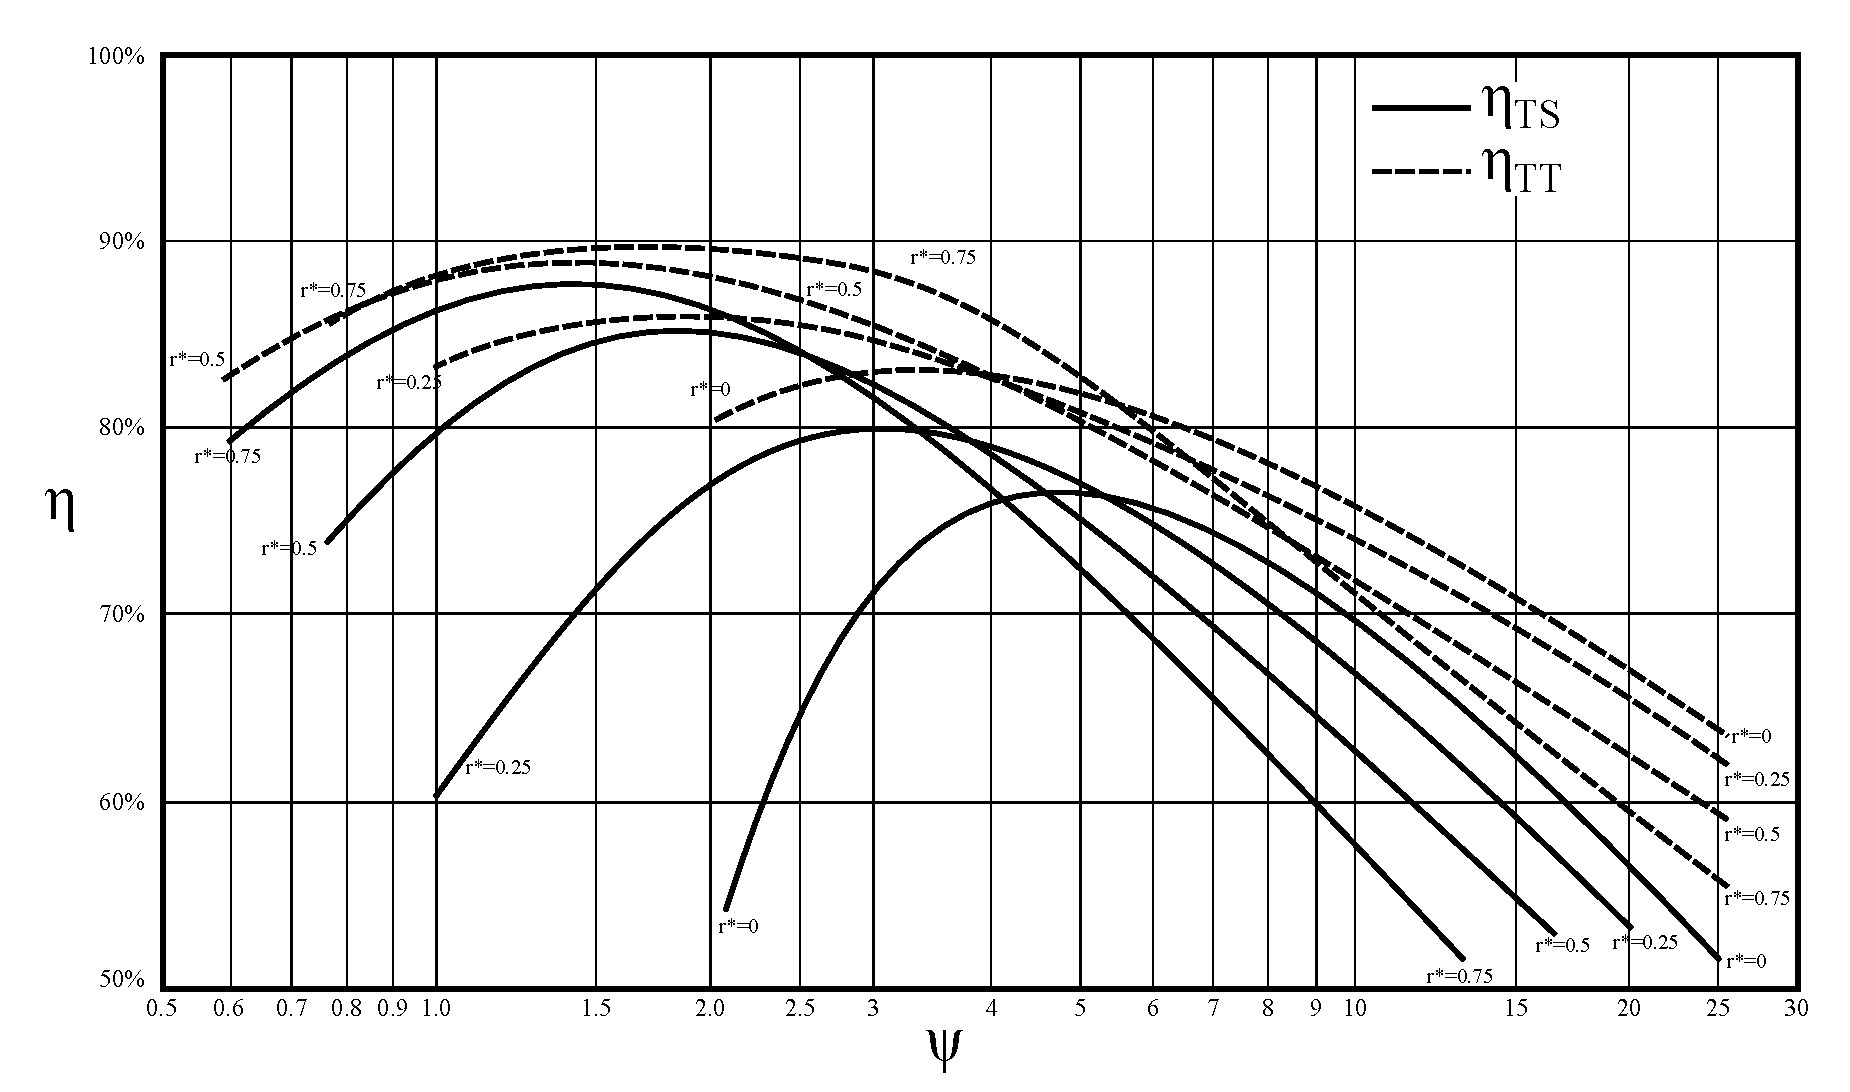
\includegraphics[width=.8\textwidth]{fig/Rendimenti_ts_tt.pdf}
\caption{}
\label{fig:Rendimenti_ts_tt}
\end{figure}
\section{Proprietà termodinamiche del flusso}
Si possono ora andare a calcolare le proprietà termodinamiche del flusso nell'attraversamento della turbina. Si definisce il numero di Mach periferico come segue
\begin{align*}
M_u = \frac{u_1}{a_{0_0}}
\end{align*}
Posso però esprimere la velocità acustica a monte della turbina in funzione dell'entalpia totale
\begin{align*}
a_{0_0} = \sqrt{kRT_{0_0}} = \sqrt{\frac{c_p}{c_v} \left( c_p - c_v \right) T_{0_0}} = \sqrt{h_{0_0} \left( k - 1 \right)}
\end{align*}

\begin{align*}
\psi	= \cfrac{h_{0_0} - h_{2ss}}{\cfrac{u_1^2}{2}} = \cfrac{c_i^2}{u_1^2} = \cfrac{\Delta h_{is_{ts}}}{\cfrac{u_1^2}{2}}
\end{align*}

\begin{align*}
\frac{c_i^2}{2} = \psi \frac{u_1^2}{2} \frac{a_{0_0}^2}{a_{0_0}^2} = \frac{\psi}{2} Mu^2 (k-1) h_{0_0}
\end{align*}
\begin{align*}
h_{1s} = h_{0_0} - \left(1- R^* \right) \frac{c_i^2}{2} = h_{0_0} \bigg[ 1- \left( 1- R^* \right) \frac{k-1}{2} \psi M_u^2 \bigg]
\end{align*}
\begin{align*}
h_{2ss} = h_{0_0} - \frac{c_i^2}{2} = h_{0_0} \bigg[ 1 - \frac{k-1}{2} \psi M_u^2 \bigg]
\end{align*}

\begin{align*}
\frac{c_1^2}{2} = \eta_s \frac{c_i^2}{2} \left( 1- R^* \right)
\end{align*}
\begin{align*}
h_1 = h_{0_0} - \frac{c_1^2}{2} = h_{0_0} \bigg[ 1- \left( 1- R^* \right) \frac{k-1}{2} \eta_s \psi M_u^2 \bigg]
\end{align*}

\begin{align*}
h_2 = h_{0_0} - \Delta h_0 - \frac{c_2^2}{2} = h_{0_0} \bigg[ 1- \bigg( \eta_{ts} + \frac{C_2^2}{\psi} \bigg) \frac{k-1}{2} \psi M_u^2 \bigg]
\end{align*}


\chapter{Compressori assiali}

\section{Introduzione}
I compressori assiali sono macchine relativamente recenti; si tratta infatti di macchine nate nel dopoguerra come componente per i gruppi turbina a gas in campo aeronautico. I primi motori aeronautici costituiti da gruppo turbogas sono stati inizialmente costruiti come compressori radiali; oggi in qualsiasi gruppo turbogas, salvo gruppo di dimensioni molto ridotte, si utilizzano compressori assiali.
\begin{figure}[h!]
\centering
  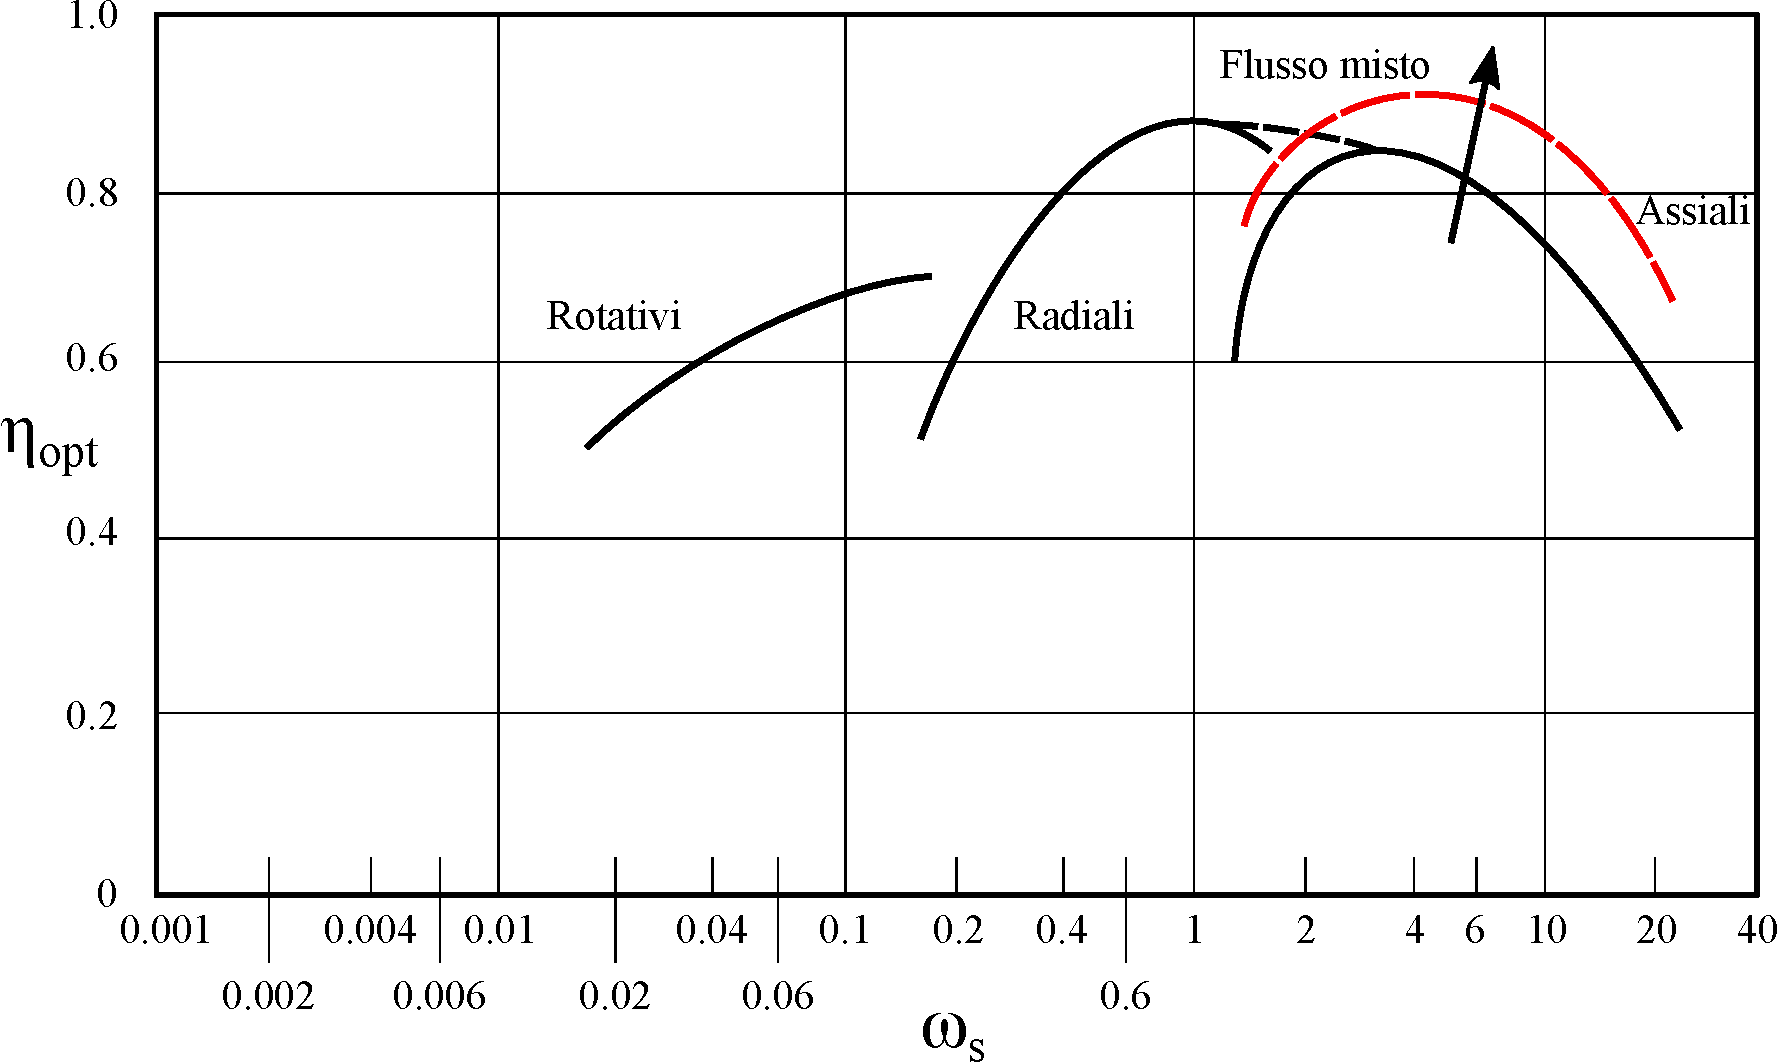
\includegraphics[width=.8\textwidth]{fig/PrestComp.pdf}
\caption{A destra le curve di rendimento per le macchine assiali. Si nota l'evidente aumento delle prestazioni (in rosso le curve per le macchine attuali) rispetto alle prime macchine.}
\label{fig:PrestComp}
\end{figure}

C'è una forte correlazione tra compressione ottenibile e rendimento. Nel diagramma in figura \ref{fig:PrestComp} è presente il rendimento del compressore in funzione della velocità specifica $\omega_s$ (che rappresenta la caratteristica di macchina) definita a partire dal coefficiente di carico $\psi$ e dal coefficiente di portata $\varphi$ ($S$ è la sezione anulare di passaggio di diametri $D_e$ e $D_i$):
\begin{align*}
\psi = \cfrac{\Delta h_{0is}}{\cfrac{u^2}{2}} \hspace{2cm} \varphi = \frac{Q}{u \cdot S}
\end{align*}
\begin{align*}
\omega_s = \cfrac{\sqrt{\varphi}}{\psi^{3/4}} \cdot \sqrt{\bigg( \cfrac{D_e}{D_i} \bigg)^2 -1}
\end{align*}
Si nota che all'aumentare della velocità specifica si va verso macchine assiali.

Fino ad un certo punto della storia le macchine assiali non hanno goduto di rendimenti competitivi; in rosso (figura \ref{fig:PrestComp}) è presentata la curva dello stato attuale dei rendimenti per macchine assiali che si vede essere maggiore rispetto quello delle prime macchine di questa tipologia. 
\begin{figure}
\centering
  \includegraphics[width=.4\textwidth]{fig/hsComp.pdf}
\caption{1: ingresso statore 2: uscita statore - entrata rotore 3: uscita statore.}
\label{fig:hsComp}
\end{figure}
\\Nel diagramma termodinamico in figura \ref{fig:hsComp} sono riportati gli stati di riferimento di uno stadio di compressore assiale. Nella parte rotorica avviene il lavoro con un relativo aumento della velocità mentre nello statore c'è il recupero in termini di pressione. Nello studio delle macchine assiali vengono fatte generalmente le seguenti assunzioni:
\begin{itemize}
\item flusso adiabatico, visto il tempo di contatto fluido-paletta molto limitato;
\item stadio ``normale" o ``ripetuto", tutti gli stadi hanno gli stessi profili:
\begin{align*}
c_1 = c_2 \;\;\;\; \Rightarrow \;\;\;\; h_3-h_1 = h_{03} - h_{01}
\end{align*}
\item velocità assiale costante (coincide con la velocità meridiana):
\begin{align*}
c_{m1} = c_{m2}
\end{align*}
\item densità costante nello stadio:
\begin{align*}
\rho = cost
\end{align*}
\end{itemize}
\section{Lavoro e triangoli di velocità}
Nel rotore si conserva la rotalpia:
\begin{equation}
h_1 + \frac{1}{2} w_1^2 = h_2 + \frac{1}{2} w_2^2
\end{equation}
Nello statore si conserva l'entalpia:
\begin{equation}
h_2 + \frac{1}{2} c_2^2 = h_3 + \frac{1}{2} c_3^2
\end{equation}
Il lavoro viene scambiato dalla parte rotorica e si definisce un parametro adimensionale per quest'ultimo ($u$ rimane costante visto che si sta trattando una macchina assiale):
\begin{equation}
\lambda = \frac{u \cdot c_{u2} - u \cdot c_{u1}}{u^2} = \frac{c_{u2} - c_{u1}}{u}
\end{equation}
\begin{figure}
\centering
  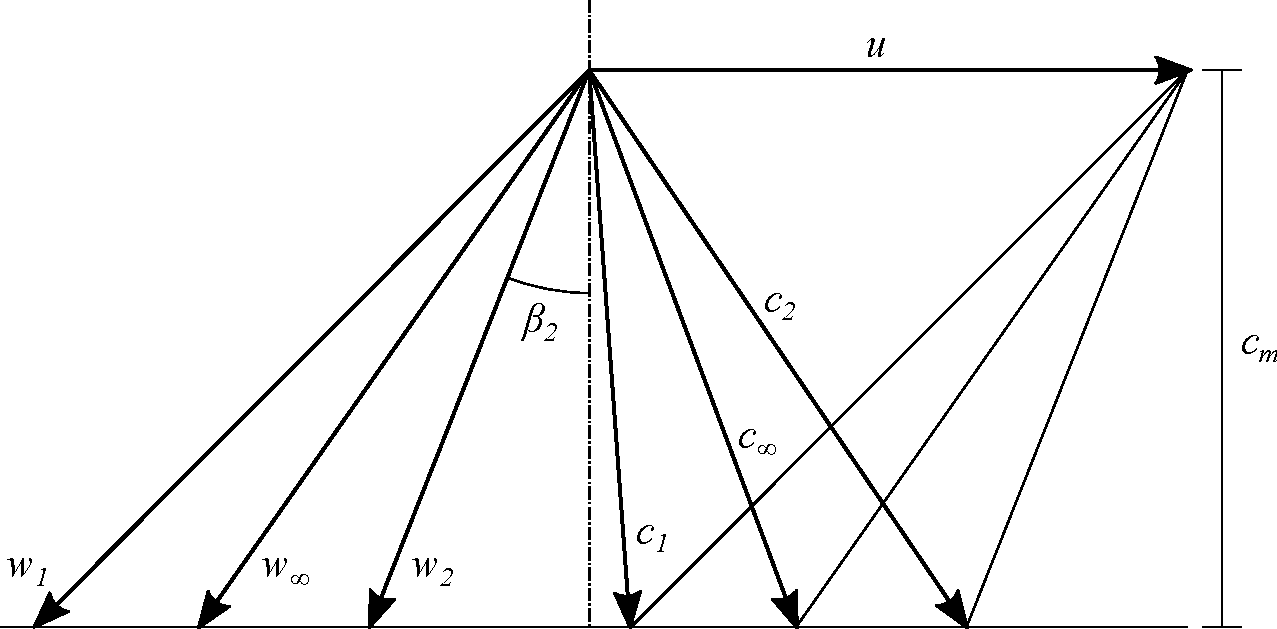
\includegraphics[width=.8\textwidth]{fig/triangComp.pdf}
\caption{}
\label{fig:triangComp}
\end{figure}
\\L'obiettivo è quello di determinare la relazione tra $\lambda$ e cifra di portata $\Phi$ definita come:
\begin{align*}
\Phi = \frac{c_m}{u}
\end{align*}
Si disegnano i triangoli di velocità relativi allo stadio elementare come mostrato in figura \ref{fig:triangComp}; per definizione la componente meridiana e periferica sono costanti. Si possono scrivere le seguenti tre relazioni:
\begin{align*}
c_{u2} = u - w_{u2}
\end{align*}
\begin{align*}
w_{u2} = c_m \tan \beta_2
\end{align*}
\begin{align*}
c_{u1} = c_m \tan \alpha_1
\end{align*}
e quindi scrivere:
\begin{align*}
\lambda = 1- \frac{w_{u2}}{u} - \frac{c_{u1}}{u} = 1 - \frac{c_m}{u} \left(\tan \beta_2 + \tan \alpha_1 \right)
\end{align*}
\'E possibile scrivere la cifra adimensionale relativa al lavoro scambiato dalla parte rotorica in funzione della cifra di portata come:
\begin{equation}
\lambda = 1 - \Phi \left( \tan \beta_2 + \tan \alpha_1 \right) = 1 - k \cdot \Phi
\end{equation}
con $k$ costante che dipende dalla geometria della macchina. Si tratta di una rappresentazione molto simile a quella del caso delle pompe centrifughe nelle quali, a seconda del valore di $k$, si ha la curva caratteristica della pompa; questo viene chiarito meglio dal diagramma in figura \ref{fig:CondProg}.
\begin{figure}
\centering
  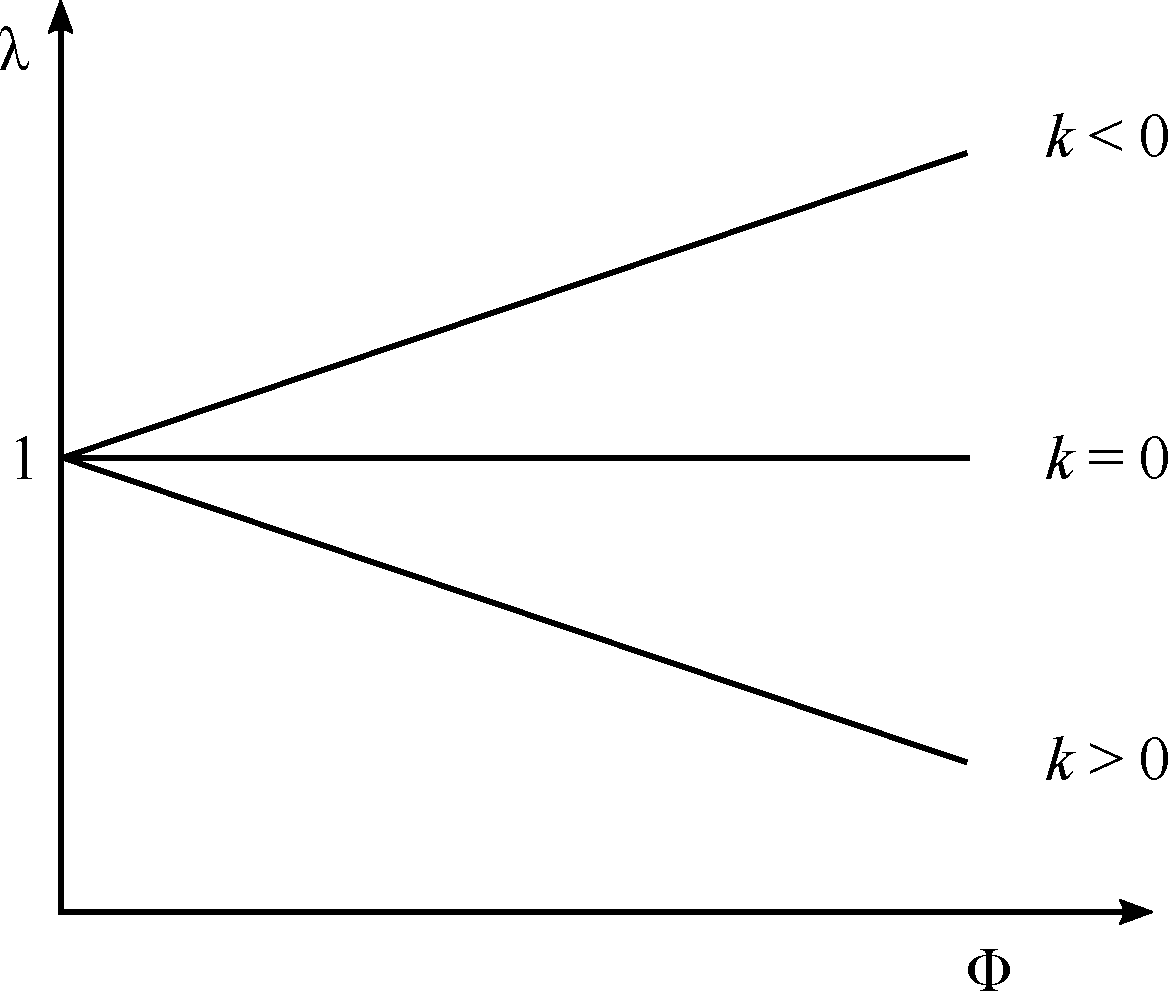
\includegraphics[width=.4\textwidth]{fig/CondProg.pdf}
\caption{}
\label{fig:CondProg}
\end{figure}
\\Si definisce una condizione particolare di progetto ``lambda di design" $\lambda_d$:
\begin{align*}
\lambda_d = 1 - k \cdot \Phi_d \;\;\;\; \rightarrow \;\;\;\; k = \frac{1}{\Phi_d}-\frac{\lambda_d}{\Phi_d}
\end{align*}
Sostituendo l'espressione di $k$ qui ricavata nella definizione generale di $\lambda$, si ottiene:
\begin{equation} \label{eq:lambdad}
\frac{\lambda}{\lambda_d} = \frac{1}{\lambda_d} - \frac{\Phi}{\Phi_d} \Bigg( \frac{1-\lambda_d}{\lambda_d} \Bigg) \;\;\;\; \text{con}\; 0.3 < \lambda_d < 0.4
\end{equation}
Si tratta di una famiglia di rette; in figura \ref{fig:LambdaPhiChart} è rappresentato il diagramma caratteristico espresso in termini di rapporti rispetto alle condizioni di progetto. Nel caso ideale di $\lambda_d = 1$ il lavoro scambiato sarebbe indipendente dalla portata, situazione abbastanza attraente ma irrealizzabile. 
\begin{figure}
\centering
\begin{minipage}{.5\textwidth}
  \centering
  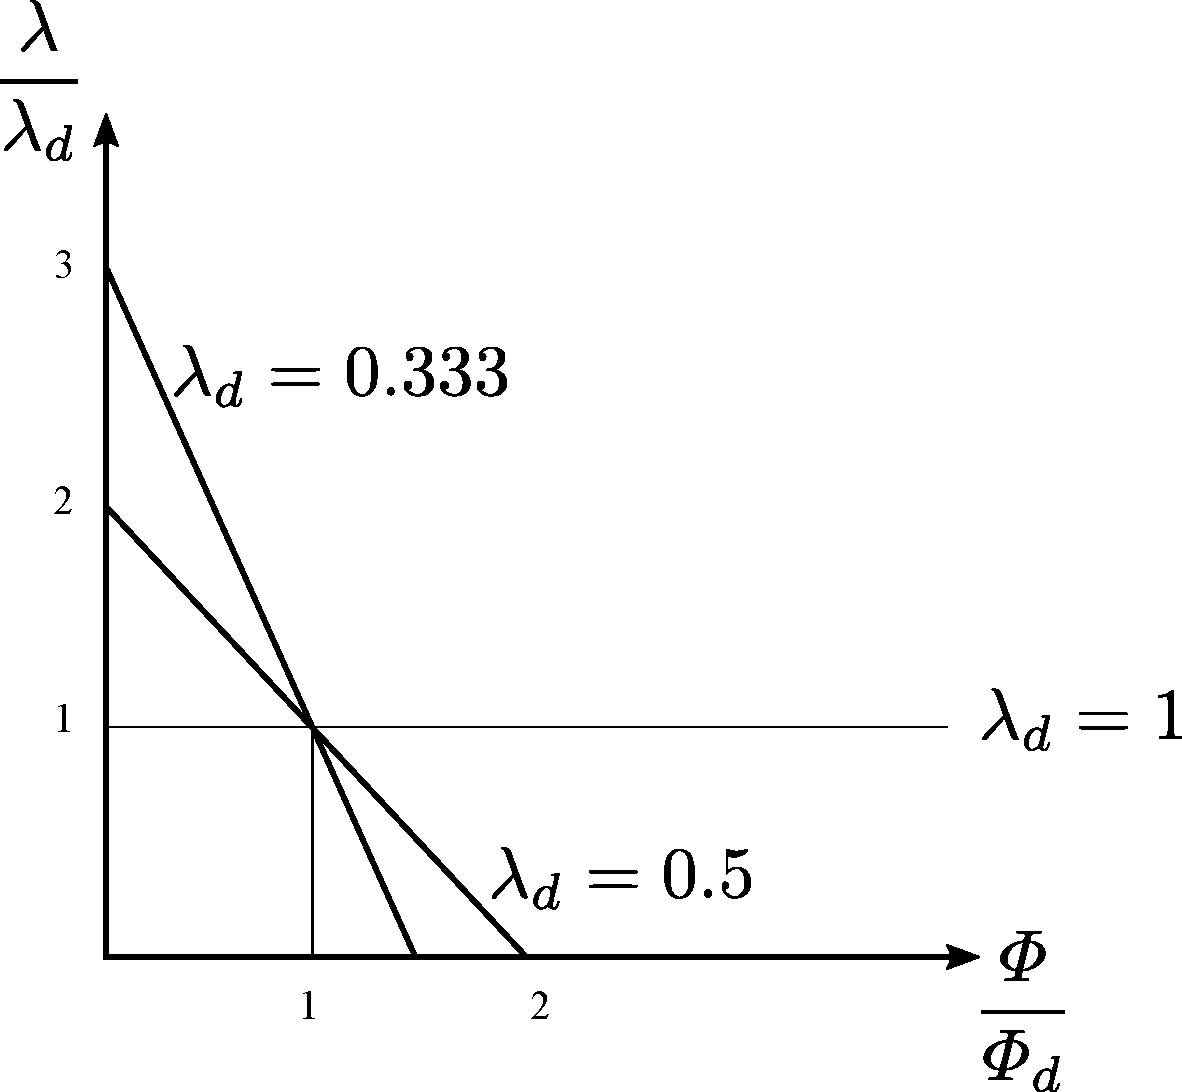
\includegraphics[width=.9\linewidth]{fig/LambdaPhiChart.pdf}
  \captionof{figure}{}
  \label{fig:LambdaPhiChart}
\end{minipage}%
\begin{minipage}{.5\textwidth}
  \centering
  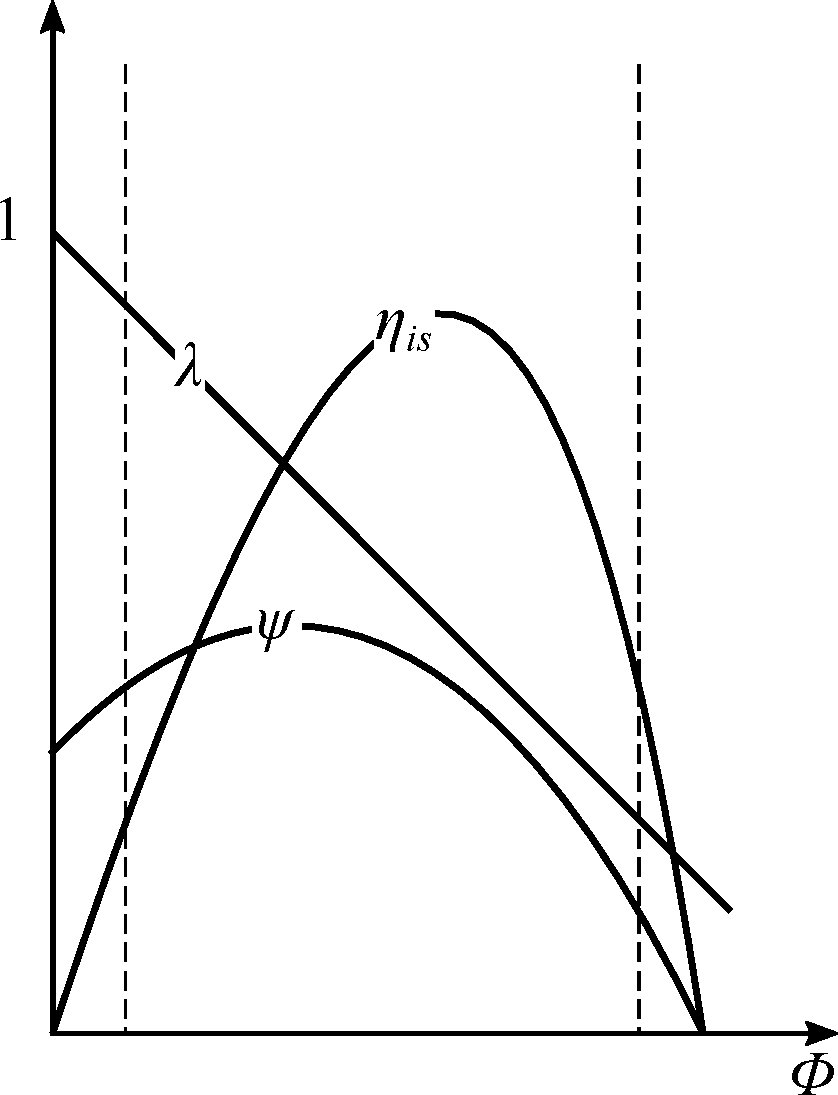
\includegraphics[width=.9\linewidth]{fig/CarattReal.pdf}
  \captionof{figure}{}
  \label{fig:CarattReal}
\end{minipage}
\end{figure}
\\Generalmente in un compressore infatti, la pressione di output è definita mentre la portata è regolata; con $\lambda_d = 1$ si otterrebbe una macchina perfetta: il rapporto di compressione si riuscirebbe sempre a mantenere e basterebbe regolare la portata per ottenere la pressione voluta. Purtroppo non è così perché le palettature non si comportano in modo ideale, si hanno separazioni di vena, inspessimenti di strato limite, ecc. Dal punto di vista realistico si riesce ad ottenere $0.3<\lambda_d<0.4$.

Come mostrato in figura \ref{fig:CarattReal} si otterrà un comportamento non ideale evidenziato dalla curva della caratteristica reale $\Psi$; essa non avrà andamento rettilineo e quindi un campo di utilizzo limitato che esclude sia portate basse che portate alte. La caratteristica reale $\Psi$ moltiplicando la caratteristica ideale per il rendimento:
\begin{equation}
\psi = \frac{\Delta h_{0is}}{u^2} = \lambda \cdot \eta_{is} \;\;\;\; \text{con}\; \Delta h_{0is} = h_{30is} - h_{10}
\end{equation}

Non è ancora stato detto nulla riguardo la forma della pala in funzione del grado di reazione definito come il rapporto tra il salto entalpico elaborato tra parte rotorica e statorica:
\begin{align*}
R = \frac{h_2 - h_1}{h_3-h_1} 
\end{align*}
Sapendo che
\begin{align*}
\begin{rcases*}
c_{u2} = u - w_{u2}\\
c_{u1} = u - w_{u1}
\end{rcases*}
\;\;\;\; \rightarrow \;\;\;\; c_{u2} - c_{u1} = w_{u1} - w_{u2} 
\end{align*}
si sviluppa l'espressione del grado di reazione della macchina applicando la conservazione della rotalpia al numeratore e l'espressione del lavoro euleriano al denominatore:
\begin{align*}
R = \frac{w_1^2 - w_2^2}{2 u (c_{u2} - c_{u1})} &= \frac{(w_{u1} + w_{u2})\cancel{(w_{u1}-w_{u2})}}{2 u \cancel{(c_{u2} - c_{u1})}} =\\
&= \frac{w_{u1} + w_{u2}}{2u} = \\
&= \frac{c_m \left(\tan \beta_1 + \tan \beta_2 \right)}{2 u}
\end{align*}
Definendo poi:
	\begin{align*}
	\tan \beta_{\infty} = \frac{\tan \beta_1 + \tan \beta_2}{2} \;\;\;\;\;\;\;\; \Phi = \frac{c_m}{u}
	\end{align*}
si ottiene
\begin{equation}
\boxed{R = \Phi \tan \beta_{\infty} = \frac{w_{u \infty}}{u}}
\end{equation}
Lo stesso risultato poteva essere raggiunto nel seguente modo:
\begin{align*}
	w_{u1} = u - c_{u1} \;\;\;\; \rightarrow \;\;\;\; R =\frac{(u-c_{u1}+w_{u2})\cancel{(w_{u1}-w_{u2})}}{2 u \cancel{(c_{u2} - c_{u1})}}=\frac{u-c_{u1}+w_{u2}}{2u}
\end{align*}
\begin{equation}
R = \frac{1}{2} + \frac{\tan \beta_2 - \tan \alpha_1}{2} \cdot \Phi \simeq \frac{1}{2} + cost \cdot \Phi
\end{equation}
Quello che è importante notare è il grado di reazione dipende tramite una costante dalla portata e che:
\begin{align*}
R = 0.5 \;\;\;\; \to \;\;\;\; \beta_2 = \alpha_1
\end{align*}
ossia che la palettatura sarà simmetrica se $R=0.5$.

Per rappresentare lo stadio al variare del grado di reazione si definiscono i triangoli di velocità (figura \ref{fig:StadioRipetuto}).
\begin{figure}
\centering
  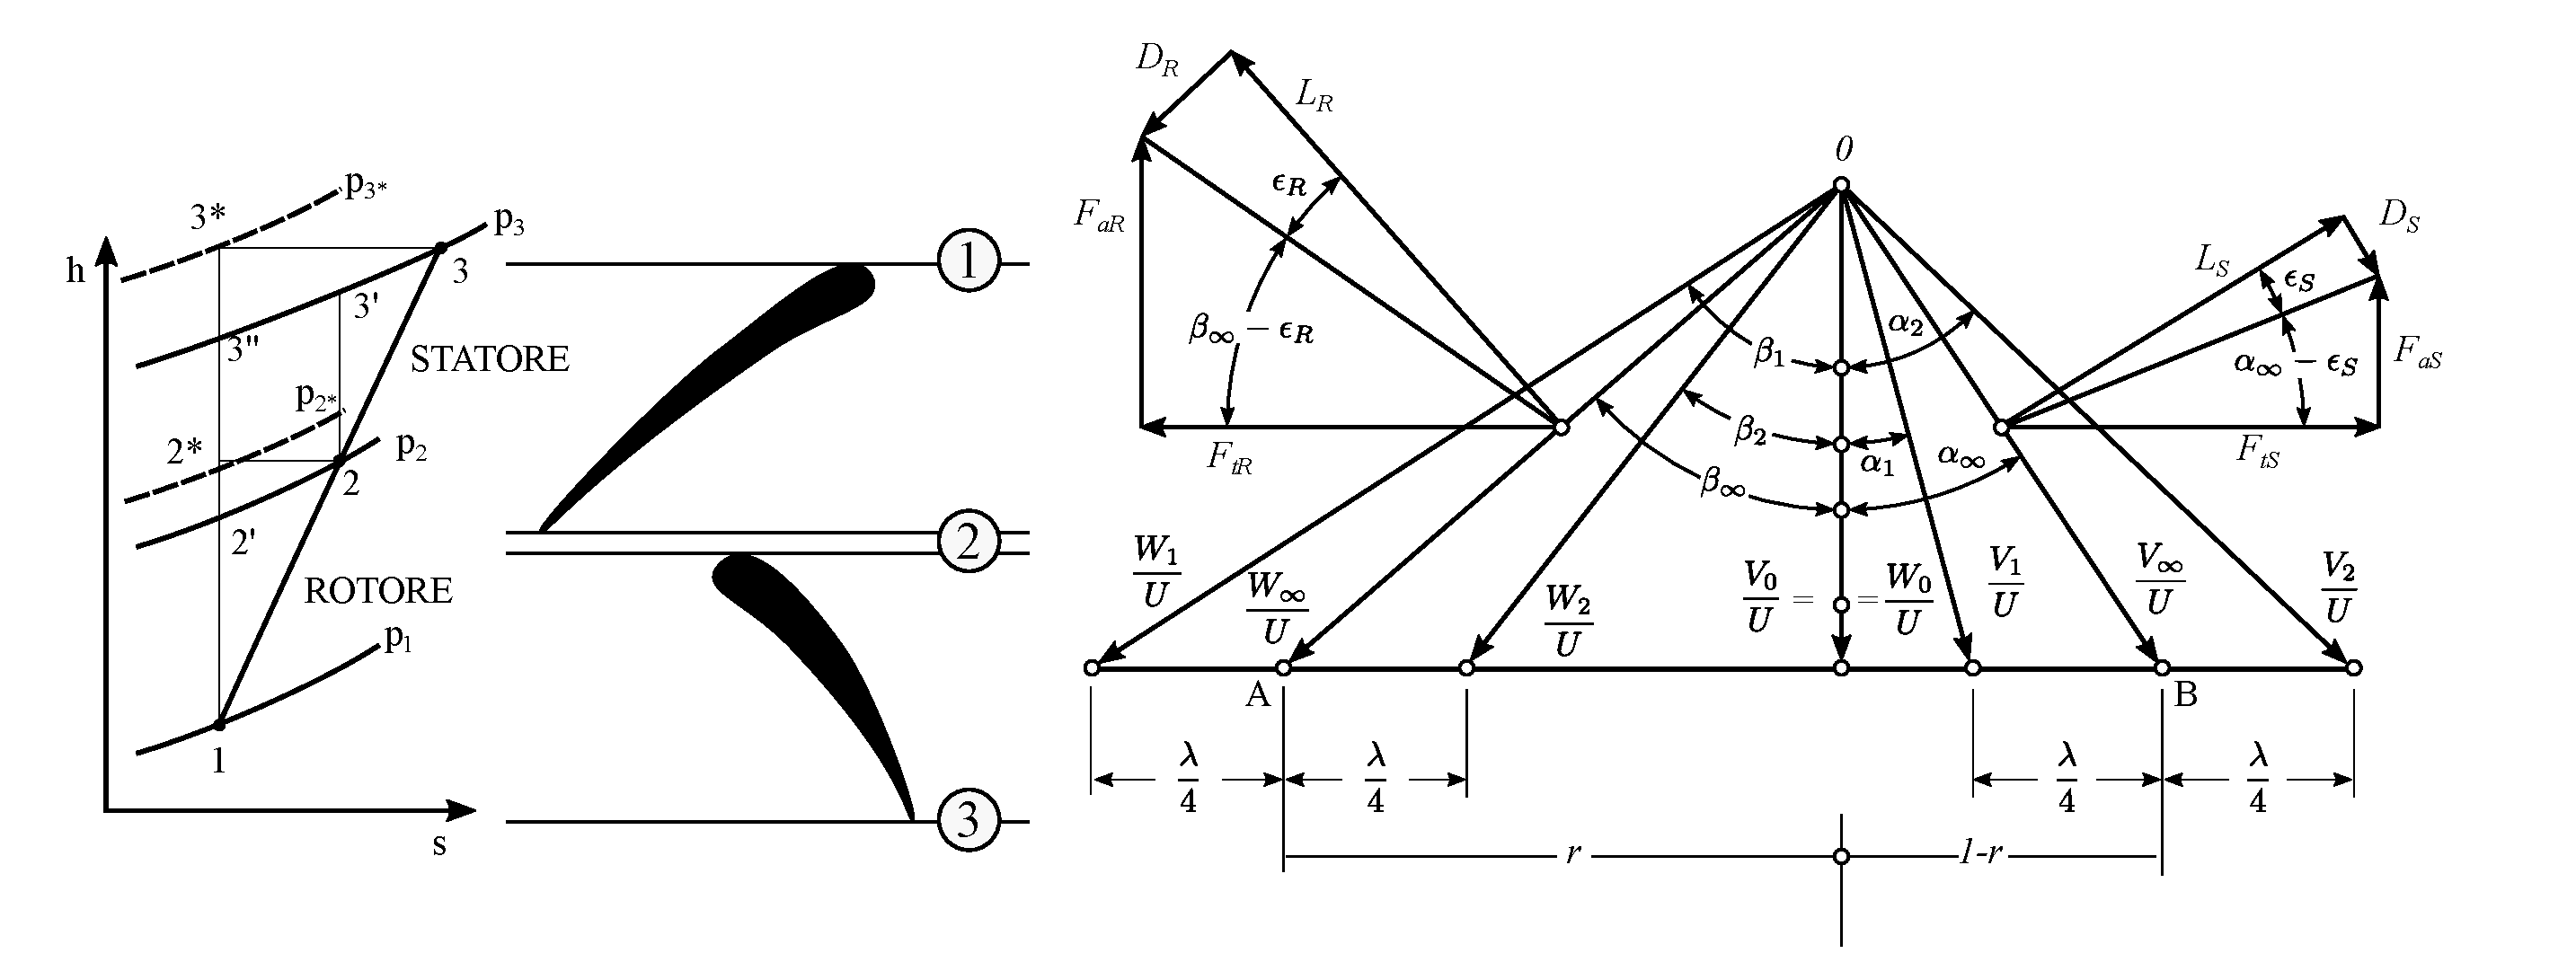
\includegraphics[width=\textwidth]{fig/StadioRipetuto.pdf}
\caption{}
\label{fig:StadioRipetuto}
\end{figure}
Facendo riferimento alla figura si può scrivere:
\begin{align*}
\Phi \cdot \tan \beta_{\infty} = R
\end{align*}
\begin{equation}\label{eq:lambda}
\lambda = \cfrac{\Delta h_0}{\cfrac{u^2}{2}} = \cfrac{u \Delta c_u}{\cfrac{u^2}{2}} = \cfrac{2 \Delta c_u}{u} = \cfrac{2 \Delta w_u}{u} \;\;\;\; \Rightarrow \;\;\;\; \frac{\Delta c_u}{u} = \frac{\Delta w_u}{u} = \frac{\lambda}{2}
\end{equation}
Qualora si operi un cambio di portata, gli unici angoli che si conservano sono $\beta_2$ e $\alpha_1$; la cifra di flusso passa dalle condizioni generiche $\Phi$ alle condizioni di design $\Phi_d$ come si vede in figura \ref{fig:CondFuoriProg}.
\begin{figure}
\centering
  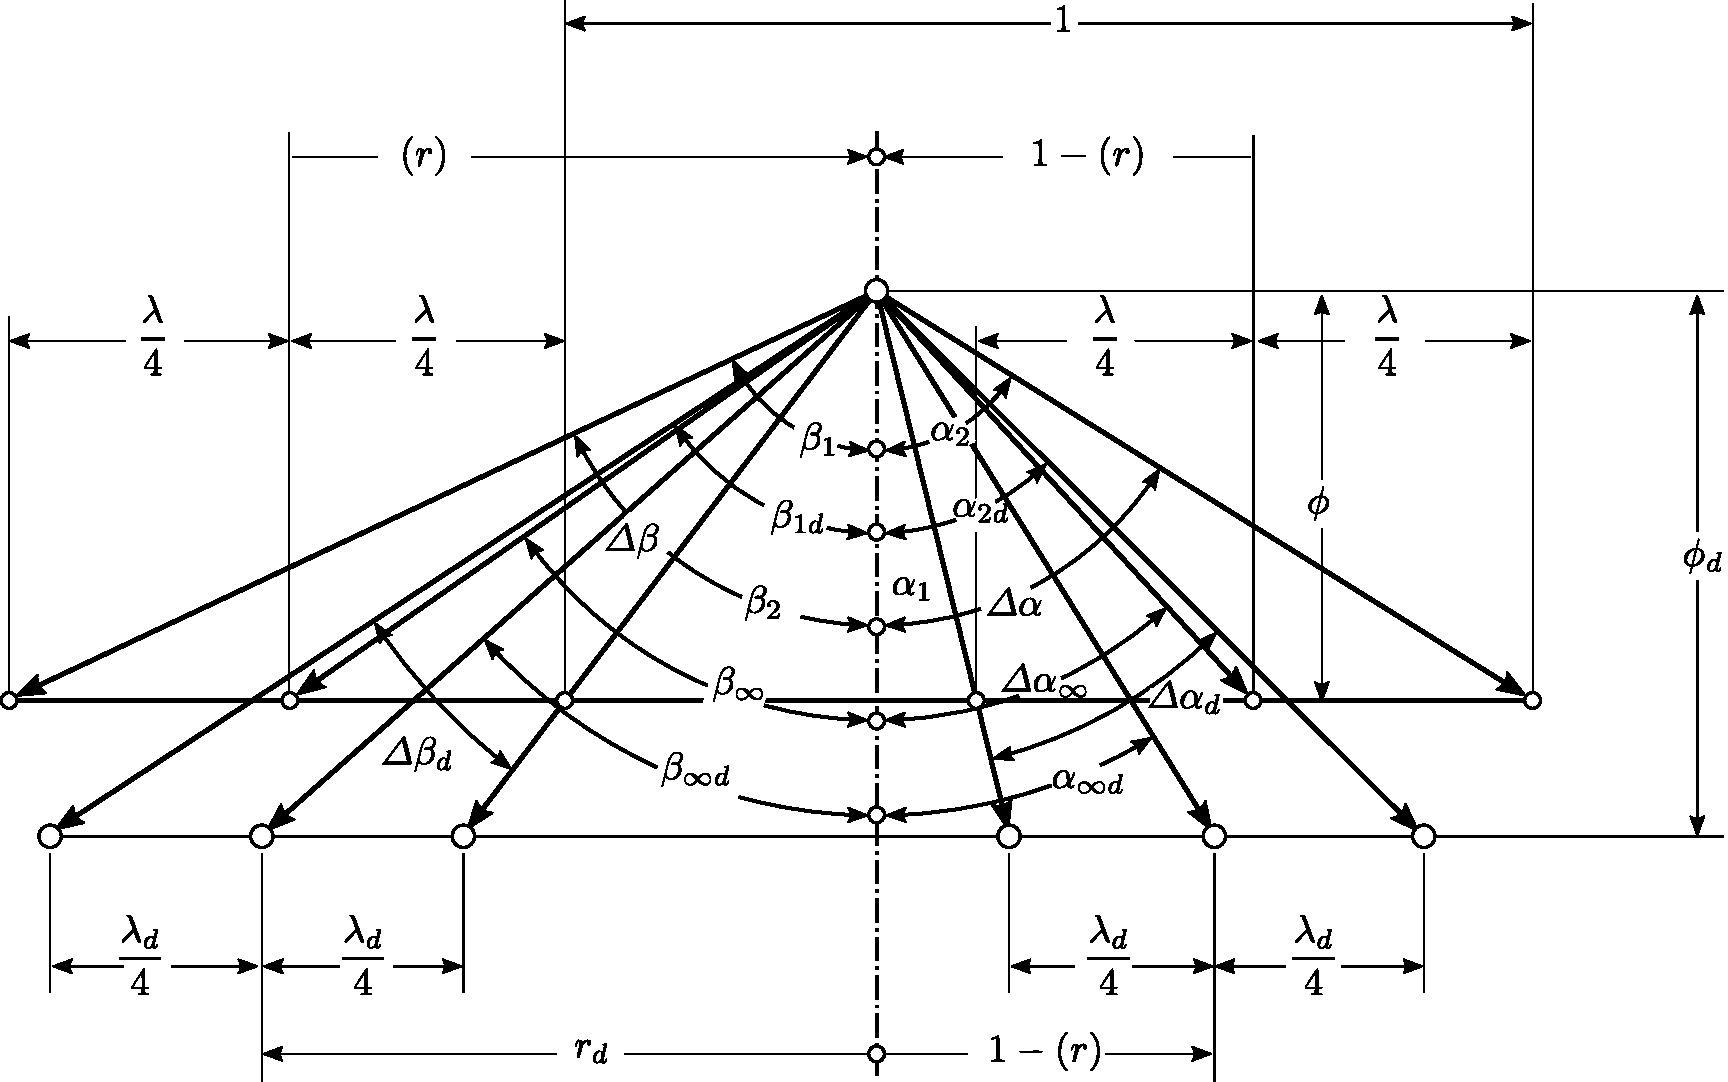
\includegraphics[width=\textwidth]{fig/CondFuoriProg.pdf}
\caption{}
\label{fig:CondFuoriProg}
\end{figure}

Si classificano alcune condizioni notevoli riportate in figura \ref{fig:ComprAssTab}:
\begin{figure}
\centering
  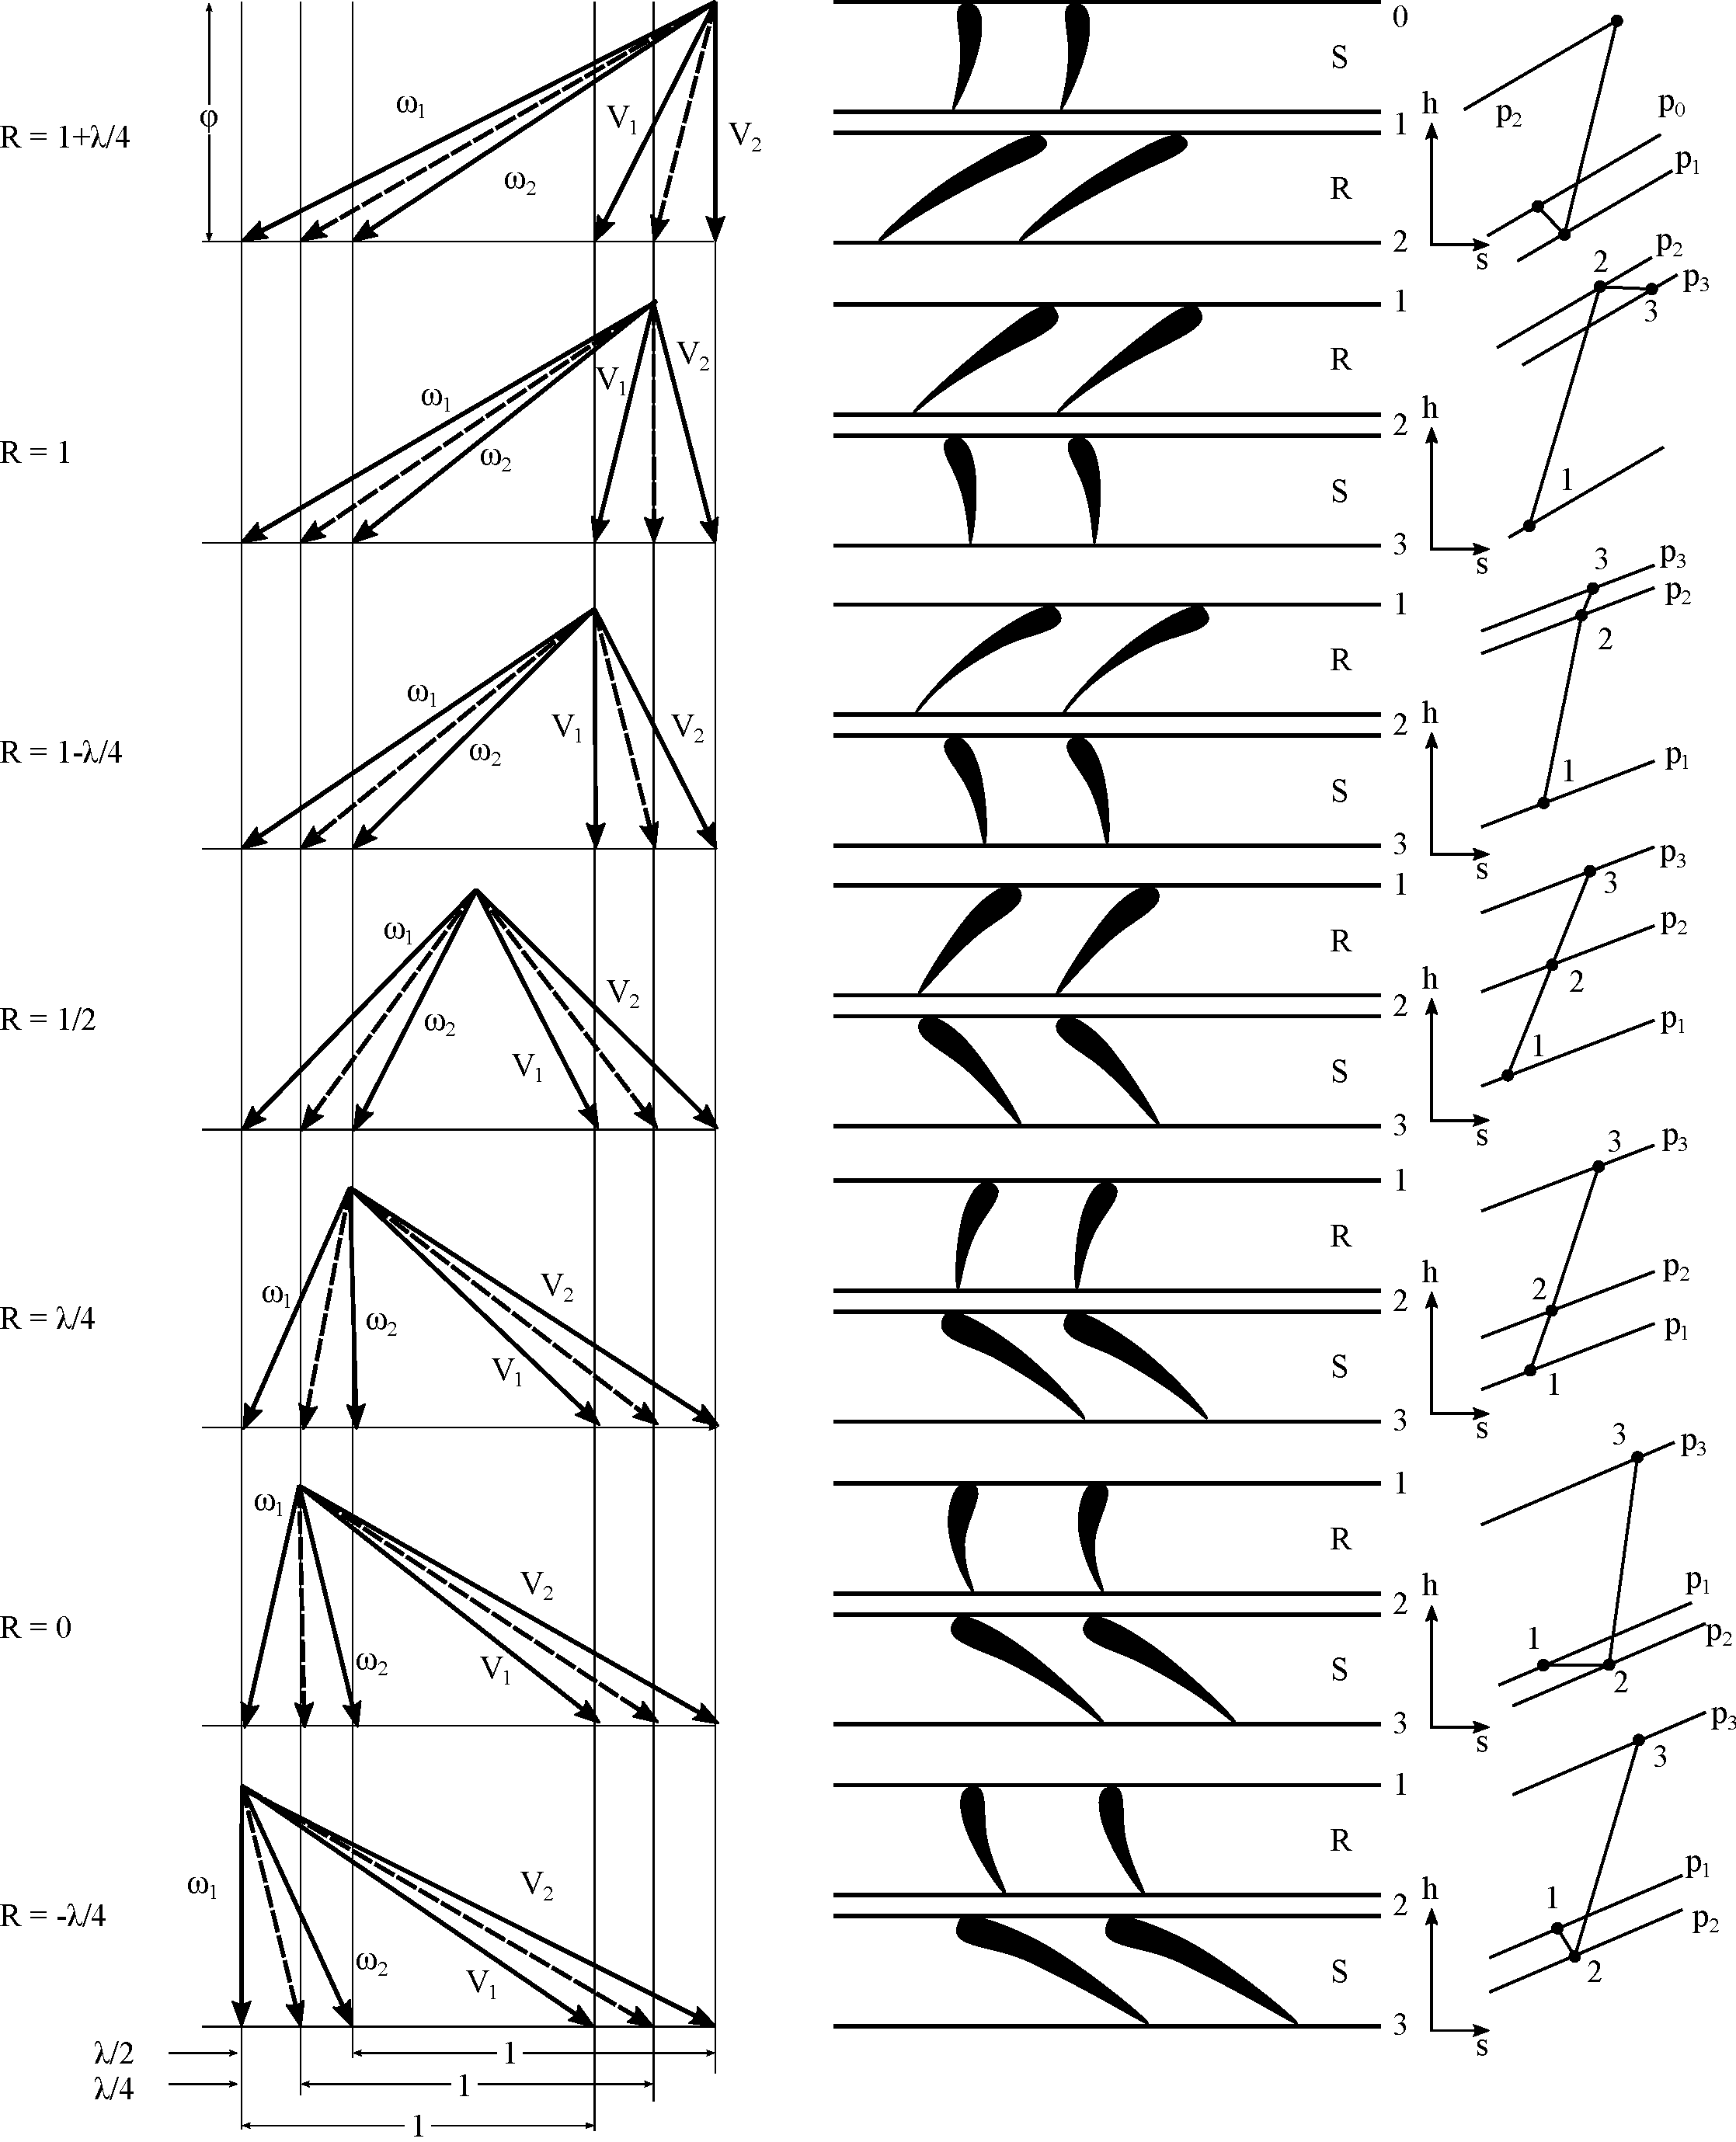
\includegraphics[width=1.2\textwidth]{fig/ComprAssTab.pdf}
\caption{}
\label{fig:ComprAssTab}
\end{figure}
\begin{itemize}
	\item il primo caso con $R = 1 + \lambda /4$ è particolare in quanto si ha grado di reazione maggiore di uno e infatti lo statore precede il rotore. In uscita sarà presente una velocità puramente assiale;

	\item con $R = 1/2$ le velocità assolute in ingresso e uscita sono simmetriche;

	\item con $R = 1 - \lambda/4$ la velocità assoluta è puramente assiale, mentre quella allo scarico non lo è;

	\item sono poi rappresentate le geometrie per gradi di reazione sempre più ridotti. 
\end{itemize}

La soluzione $R = 1/2$ è la più diffusa e utilizzata eccetto per il primo e l'ultimo stadio in cui si vogliono distribuzioni di velocità particolari (si usano rispettivamente $R = 1 - \lambda /4$ e $R = 1 + \lambda /4$). In questa configurazione si avranno profili uguali ma specchiati e l'incremento di pressione (da $p_1$ a $p_3$) è diviso equamente in due parti uguali tra la parte statorica e la parte rotorica. 

\section{Termodinamica}
Si calcola il rendimento al variare della portata e del grado di reazione. Si definisce il rendimento isoentropico:
\begin{align*}
\eta_{is} = \frac{\Delta h_{is}}{\Delta h_0}
\end{align*}
Dal primo principio della termodinamica:
\begin{align*}
T ds = dh - \frac{dp}{\rho}
\end{align*}
ma
\begin{align*}
ds = 0 \;\;\;\; \rightarrow \;\;\;\; dh = \frac{dp}{\rho}
\end{align*}
Si ottiene, considerando la definizione \ref{eq:lambda} di $\lambda$, quindi:
\begin{equation}\label{eq:etadp}
\eta_{is} = \frac{\Delta p}{\rho \cdot \Delta h_0} = \cfrac{\Delta p}{\rho \cdot \cfrac{\lambda}{2} u^2}
\end{equation}
Considerando i triangoli di velocità (figura \ref{fig:StadioRipetuto}), l'incremento di pressione totale si può ulteriormente sviluppare come somma di incremento di pressione sviluppato nel rotore e nello statore:
\begin{equation}
\Delta p = \Delta p_R + \Delta p_S = \frac{F_{aR}}{s_R} + \frac{F_{aS}}{s_S} = \frac{F_{tR} \cdot \tan(\beta_{\infty} - \varepsilon_R)}{s_R} + \frac{F_{tS} \cdot \tan(\alpha_{\infty} - \varepsilon_S)}{s_S}
\label{eq:deltap}
\end{equation}
con $\varepsilon_S$ e $\varepsilon_R$ indici di efficienza del profilo e $s_R$ e $s_S$ i passi\footnote{Per quanto riguarda i pedici "S" sta per statore, "R" per rotore.}.\\
Si può fare qualche assunzione: i profili hanno drag molto più piccolo del lift quindi:
\begin{align*}
\tan \varepsilon_R \simeq \varepsilon_R = \frac{D_R}{L_R} \;\;\;\;\;\;\;\; \tan \varepsilon_S \simeq \varepsilon_S = \frac{D_S}{L_S}
\end{align*}
Utilizzando le componenti di forza del triangolo di velocità per rotore e statore, e ricordando la definizione di $\Phi$, si ottiene:
\begin{align*}
F_{tR} = \dot{m} \cdot \Delta w_u = \overbrace{s_R \cdot \rho \cdot c_m}^\text{$ \dot{m} $} \cdot \overbrace{\lambda \cdot u \cdot \frac{1}{2}}^\text{$\Delta w_u$}=  s_R \cdot \rho \cdot \lambda \cdot \Phi \cdot u^2 \cdot \frac{1}{2}
\end{align*}
\begin{align*}
F_{tS} = \dot{m} \cdot \Delta c_m = s_S \cdot \rho \cdot c_m \cdot \lambda \cdot u \cdot \frac{1}{2} =s_S \cdot \rho \cdot \lambda \cdot \Phi \cdot u^2 \cdot \frac{1}{2}
\end{align*}
Andando a sostituire le due forze nell'equazione \ref{eq:deltap}:
\begin{align*}
\Delta p = \frac{1}{2} \rho \lambda u^2 \big[ \Phi \tan \left( \beta_{\infty} - \varepsilon_R \right) + \Phi \tan \left( \alpha_{\infty} - \varepsilon_S \right) \big] 
\end{align*}
e ricordando le relazioni
\begin{align*}
R = \Phi \tan \beta_{\infty} \;\;\;\;\;\;\;\;\;\;\; 1 - R = \Phi \tan \alpha_{\infty} 
\end{align*}
\begin{align*}
\tan ( \beta_{\infty} - \varepsilon_R ) = \frac{\tan \beta_{\infty} - \tan \varepsilon_R}{1 + \tan \beta_{\infty} \tan \varepsilon_R} \simeq \frac{\tan \beta_{\infty} - \varepsilon_R}{1 + \tan \beta_{\infty} \varepsilon_R}= \frac{R - \varepsilon_R \Phi}{\Phi + \varepsilon_R R}
\end{align*}
\begin{align*}
\tan (\alpha_{\infty} - \varepsilon_S) \simeq \frac{\tan \alpha_{\infty} - \varepsilon_S}{1 + \tan \alpha_{\infty} \cdot \epsilon_S} = \frac{1 - R - \varepsilon_S \Phi}{\Phi + \varepsilon_S (1-R)}
\end{align*}
Si ottiene infine la relazione del salto di pressione in funzione del grado di reazione e di $\lambda$:
\begin{equation}
\Delta p = \frac{1}{2} \rho \lambda u^2 \Bigg[ \frac{R - \varepsilon_R \Phi}{\Phi + \varepsilon_R R} + \frac{1 - R - \varepsilon_S \Phi}{\Phi + \varepsilon_S (1-R)} \Bigg] \cdot \Phi
\end{equation}
Il rendimento isoentropico, ricordando l'equazione \ref{eq:etadp}, diviene:
\begin{equation}
\boxed{ \eta_{is} = \Bigg[ \frac{R - \varepsilon_R \Phi}{\Phi + \varepsilon_R R} + \frac{1 - R - \varepsilon_S \Phi}{\Phi + \varepsilon_S (1-R)} \Bigg] \cdot \Phi }
\end{equation}
Si introduce una semplificazione sugli indici di efficienza e si cerca il coefficiente di reazione ottimale:
\begin{align*}
\varepsilon_S \simeq \varepsilon_R = cost = \varepsilon
\end{align*}
\begin{align*}
\frac{d \eta_{is}}{dR} = 0 \;\;\;\; \text{se}  \;\;\;\; R_{opt} = 0.5 \mbox{ per } \forall \Phi
\end{align*}
Il rendimento con questo valore di R vale:
\begin{align*}
\eta_{|R= 0.5} = 2 \Phi \cdot \frac{1- 2 \varepsilon \Phi}{\varepsilon + 2 \Phi}
\end{align*}
Il rendimento del compressore è migliorato alla diminuzione di $\varepsilon$. Questa relazione lega quindi il rendimento alla portata e all'efficienza del profilo; per il progetto di un compressore si inizierà quindi dallo studio del singolo profilo visto che le sue prestazioni hanno influenza sul rendimento totale\\
Si determina ora il valore di $\Phi$ che rende massimo il rendimento ottimale:
\begin{align*}
\frac{d\eta_{|R=0.5}}{d \Phi} = 0 \;\;\;\; \text{se} \;\;\;\; \Phi_{opt} = \frac{1}{2} \left( \sqrt{1 + \varepsilon^2} - \varepsilon \right) \simeq \frac{1 - \varepsilon}{2}
\end{align*}
\begin{equation}
\eta_{max} = 1 + 2 \varepsilon^2 - 2 \varepsilon \sqrt{1 + \varepsilon^2} \simeq 1 - 2 \varepsilon \left( 1 - \varepsilon \right)
\end{equation}
\begin{figure}
\centering
  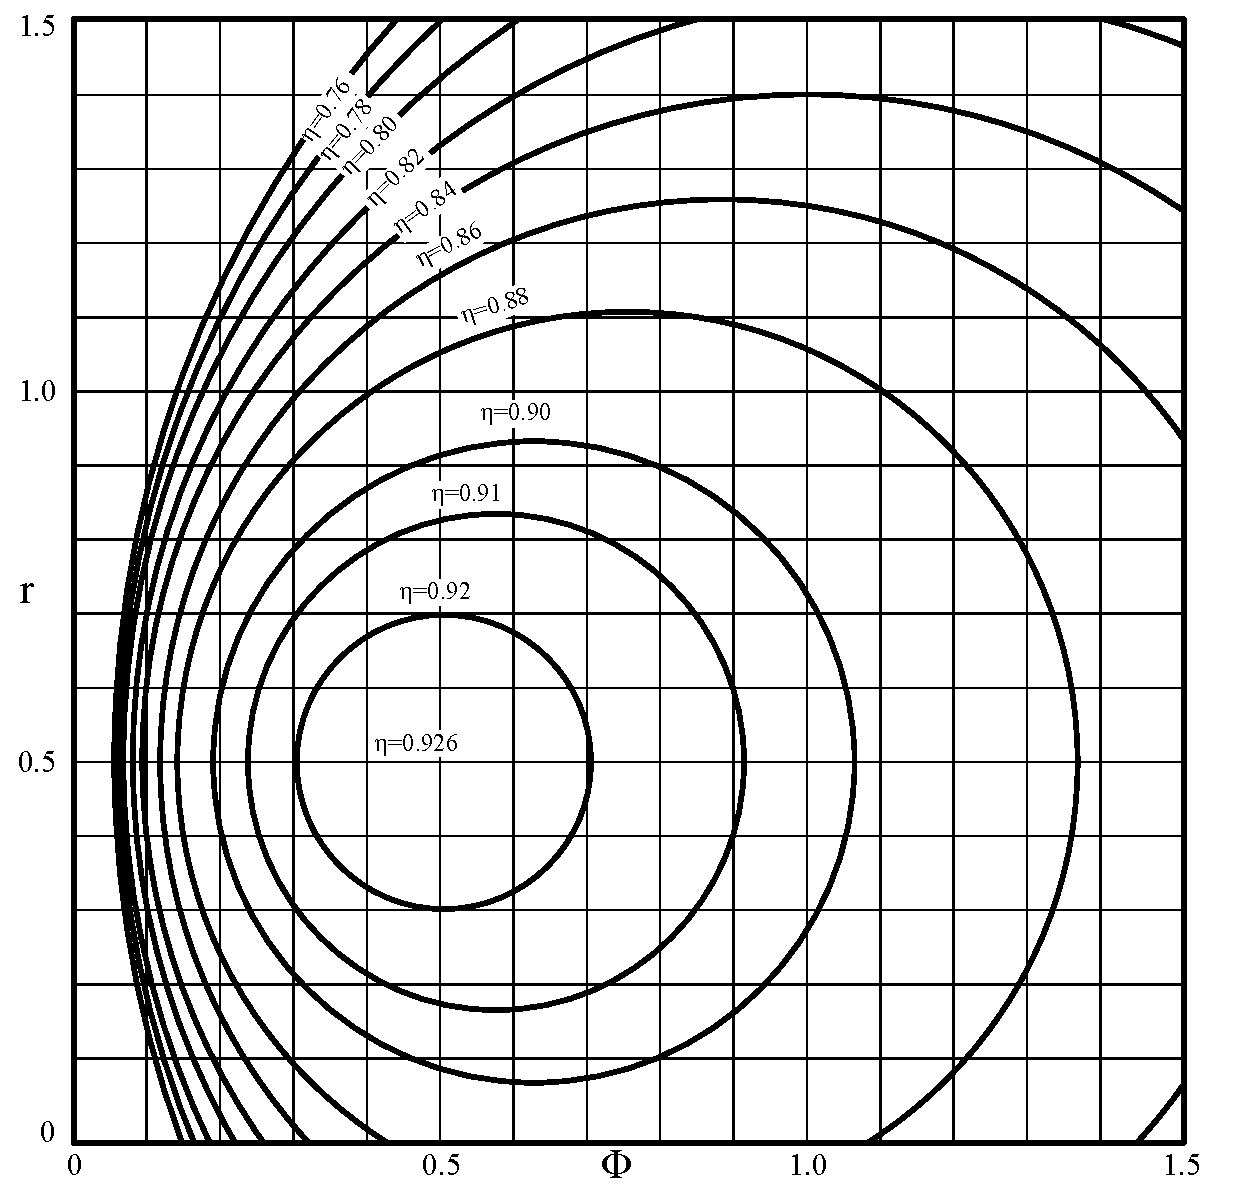
\includegraphics[width=\textwidth]{fig/IsoRendCompAss.pdf}
\caption{Curve isorendimento di uno stadio assiale in funzione del grado di reazione e coefficiente di portata per efficienza del profilo $\epsilon=0.04$}
\label{}
\end{figure}

\section{Progettazione della schiera}
Sono presenti molteplici correlazioni per progettare una macchina assiale. Si analizzeranno un filone di correlazioni datate ma che non hanno perso di validità. Anche nella progettazione di una nuova macchina è utile partire da un predimensionamento per poi andare a raffinare lo studio con strumenti moderni. Queste correlazioni verranno quindi usate come passo preliminare.\\
\'E possibile fare le seguenti riflessioni:
\begin{itemize}
\item la deflessione imposta alla corrente è limitata: nell'ordine delle decine di gradi ($20 \div 30$ al massimo $40$);
\item profili sottili a bassa curvatura.
\end{itemize}
Le perdite possono quindi essere suddivise in:
\begin{itemize}
\item perdite di anello: sono dovute all'interazione tra flusso elicoidale che si sviluppa all'interno del compressore e la cassa della macchina. Esse inducono un drag aggiuntivo correlato a quanto più è elevato lo sviluppo radiale della pala. Definito $H$ lo sviluppo radiale e $s$ passo palare, si può scrivere:
\begin{align*}
C_{Da} = 0.02 \cdot \frac{s}{H}
\end{align*}
\item perdite di profilo: sono direttamente correlate al coefficiente $c_D$, saranno quelle in cui si può andare maggiormente a lavorare;
\item perdite per flussi secondari: trattate nel capitolo precedente. Esse sono dipendono dal quadrato del coefficiente di portanza; tanto più la portanza è elevata tanto verrà imposta una deviazione e di conseguenza tanto più è probabile che si instaurino moti secondari.
\begin{align*}
C_{Ds} = 0.018 \cdot c_L^2
\end{align*}
\end{itemize}
\'E possibile andare quindi a scrivere un coefficiente di resistenza complessivo:
\begin{equation}
C_{Dtot} = C_D + C_{Da} + C_{Ds} = C_D + 0.02 \cdot \frac{s}{H} + 0.018 \cdot c_L^2
\label{eq:Cdtot}
\end{equation}
In questo modo si riconducono le perdite all'interno del flusso ad un incremento del coefficiente di resistenza del profilo. In figura \ref{fig:ComprStageLoss} si vede come le varie perdite inficino sull'efficienza della schiera.
\begin{figure}
\centering
  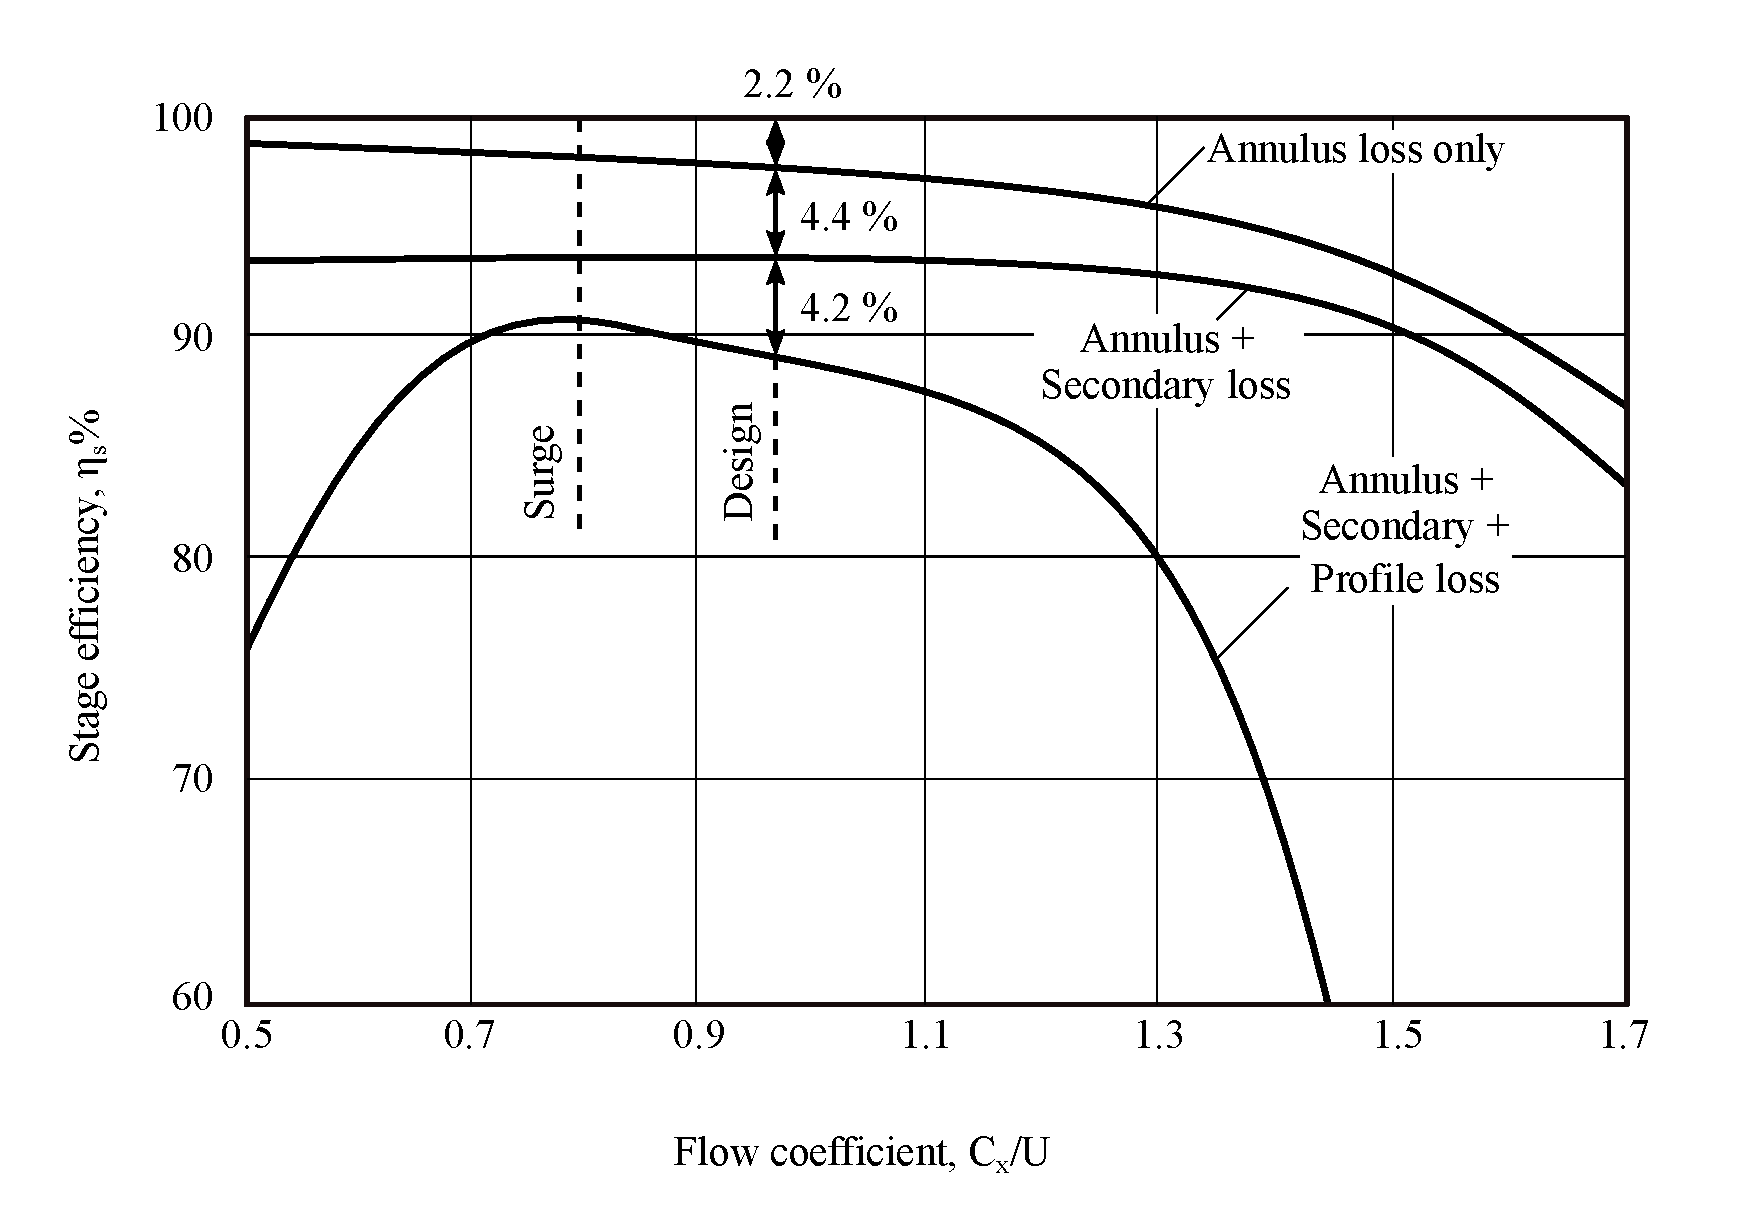
\includegraphics[width=\textwidth]{fig/ComprStageLoss.pdf}
\caption{}
\label{fig:ComprStageLoss}
\end{figure}
\subsection{Correlazioni di Howell}
Si ricordano le nomenclature utilizzate in questo capitolo in figura \ref{fig:SchieraDim}; in particolare è evidenziata la differenza tra angoli geometrici e fluidodinamici.
\begin{figure}
	\centering
	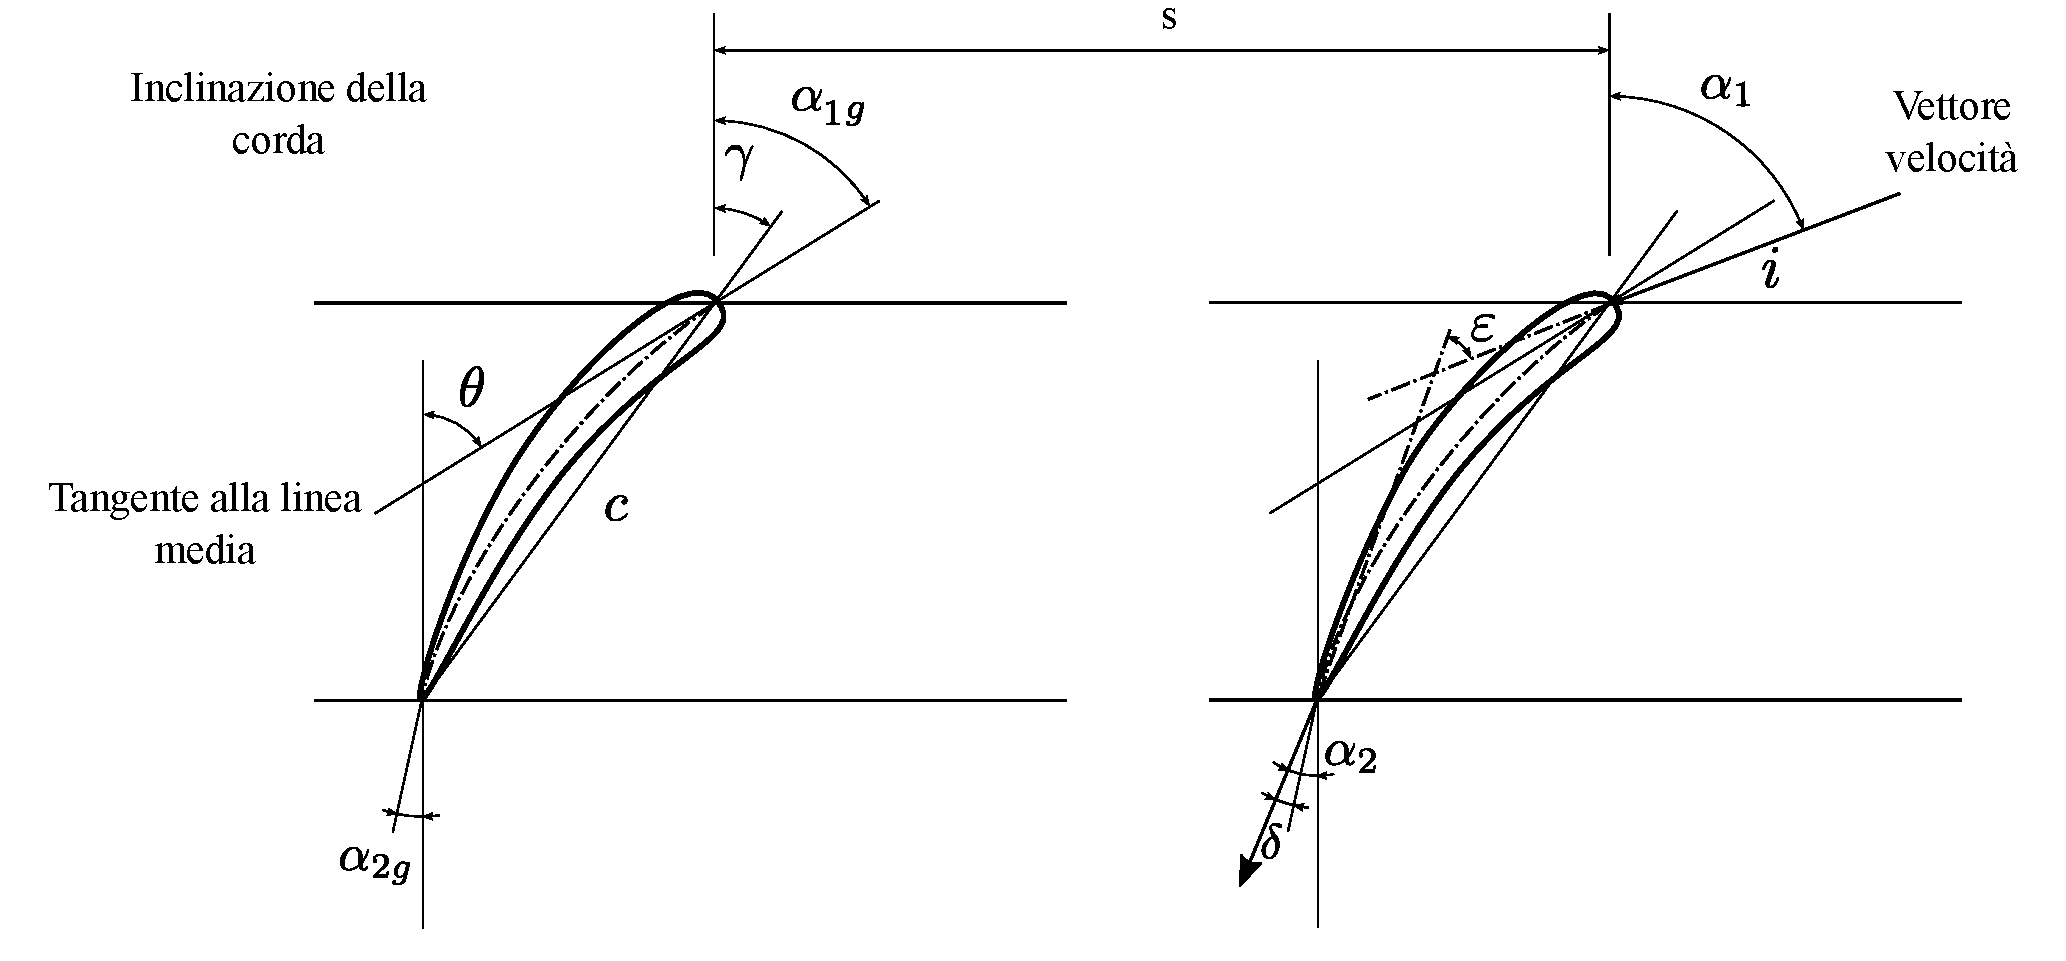
\includegraphics[width=\textwidth]{fig/SchieraDim.pdf}
	\caption{}
	\label{fig:SchieraDim}
\end{figure}

Nella progettazione preliminare fatta utilizzando la correlazione di Howell, si va a cercare la relazione tra gli angoli geometrici in ingresso e in uscita e gli angoli che deve avere il fluido.

La correlazione di Howell dice che la condizione di riferimento, ovvero la deflessione nominale che la corrente subisce nell'attraversamento delle pale $\varepsilon^*$, dipende dalla deviazione di stallo $\varepsilon_s$:
\begin{equation}
\varepsilon^* = 0.8 \cdot \varepsilon_s
\end{equation}
In figura \ref{fig:Howell} è rappresentato l'andamento della deflessione in funzione dell'angolo di incidenza. Come si nota è presente un tratto pressoché lineare seguito da un brusco cambiamento di curvatura dovuto allo stallo. Quest'ultimo è facilmente individuabile e risulta quindi comodo utilizzarlo come punto di riferimento per individuare la deflessione nominale. Come deflessione nominale si utilizzerà quindi un valore che va a minimizzare le perdite, tenendo conto poi dei margini di operabilità.  
\begin{figure}
\centering
  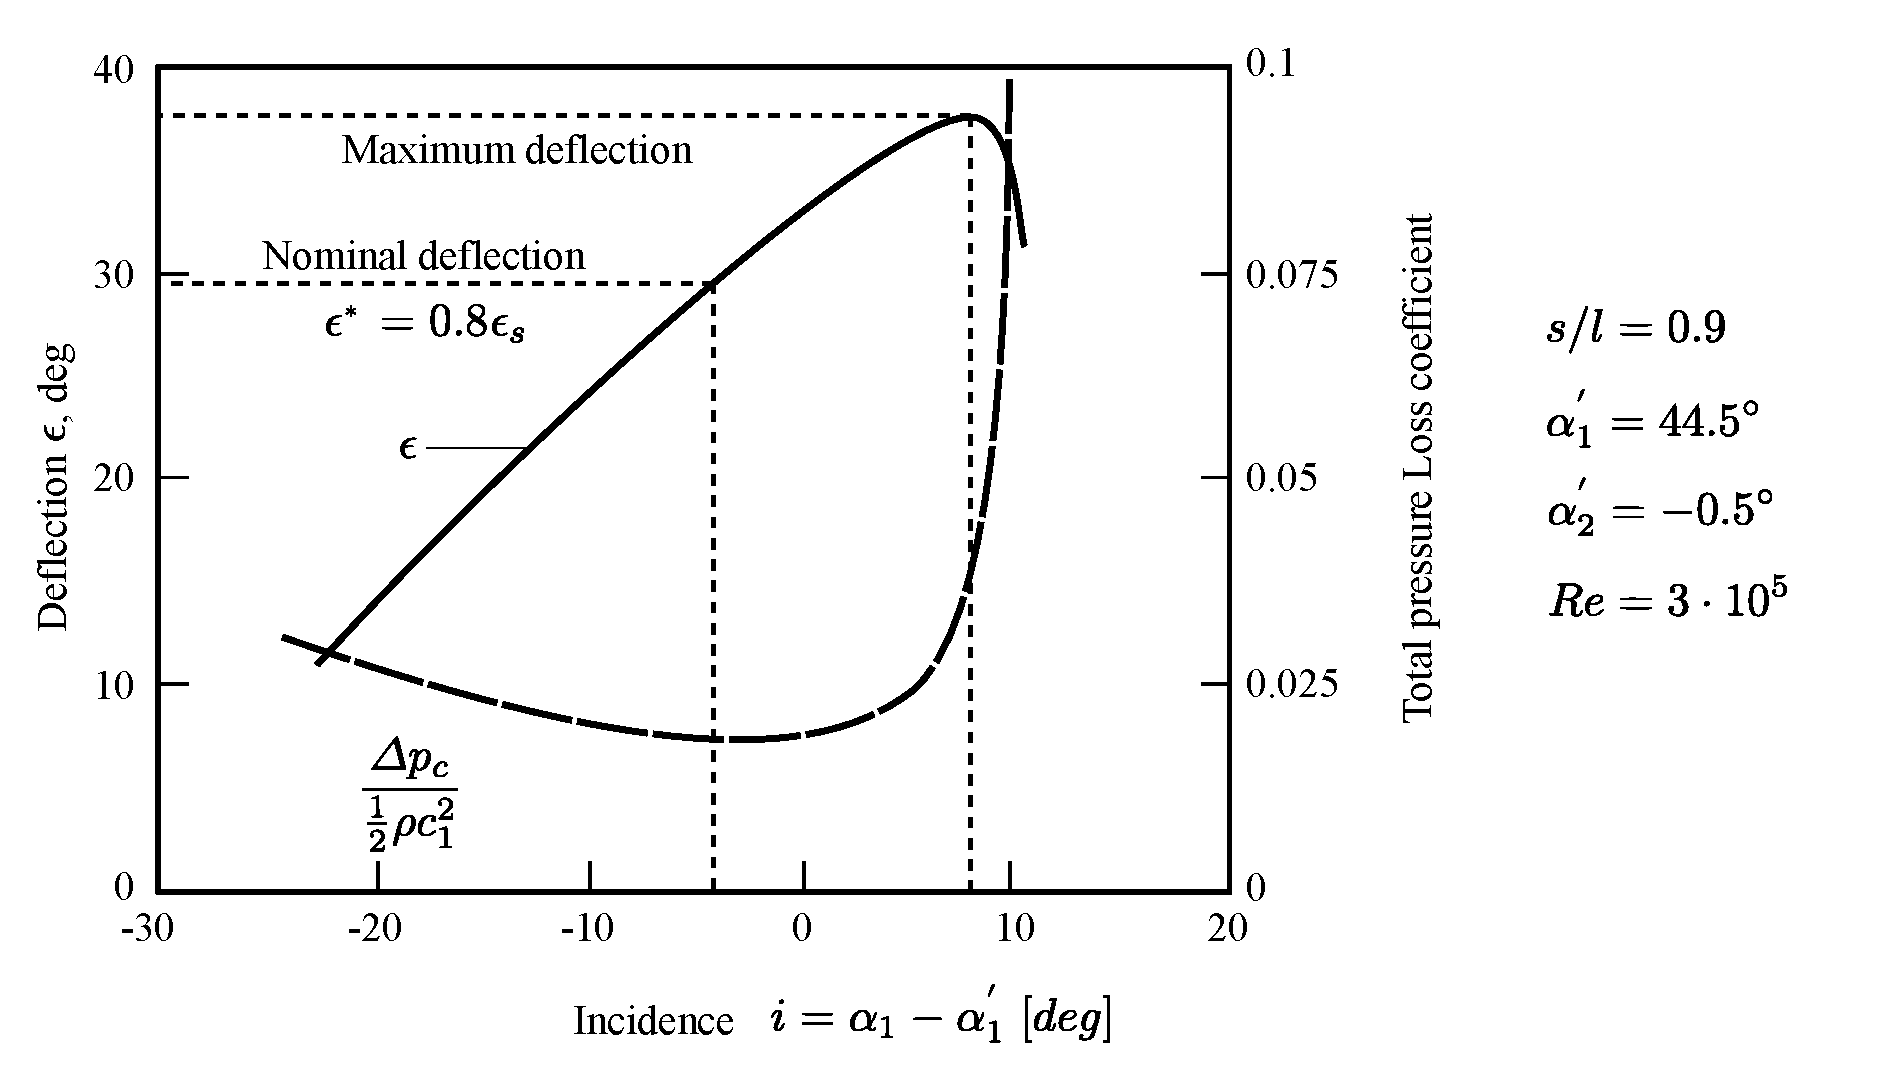
\includegraphics[width=\textwidth]{fig/Howell.pdf}
\caption{}
\label{fig:Howell}
\end{figure}

La prima correlazione di Howell permette di calcolare gli angoli del flusso attesi da una schiera di data solidità ($\epsilon=\epsilon^*$). Questa viene riportata in figura \ref{fig:1CorrHowell} al variare della solidità della schiera. Si nota che a parità di deflessione nominale si avrà una maggiore angolo in uscita per schiere più compatte.
\begin{figure}
	\centering
	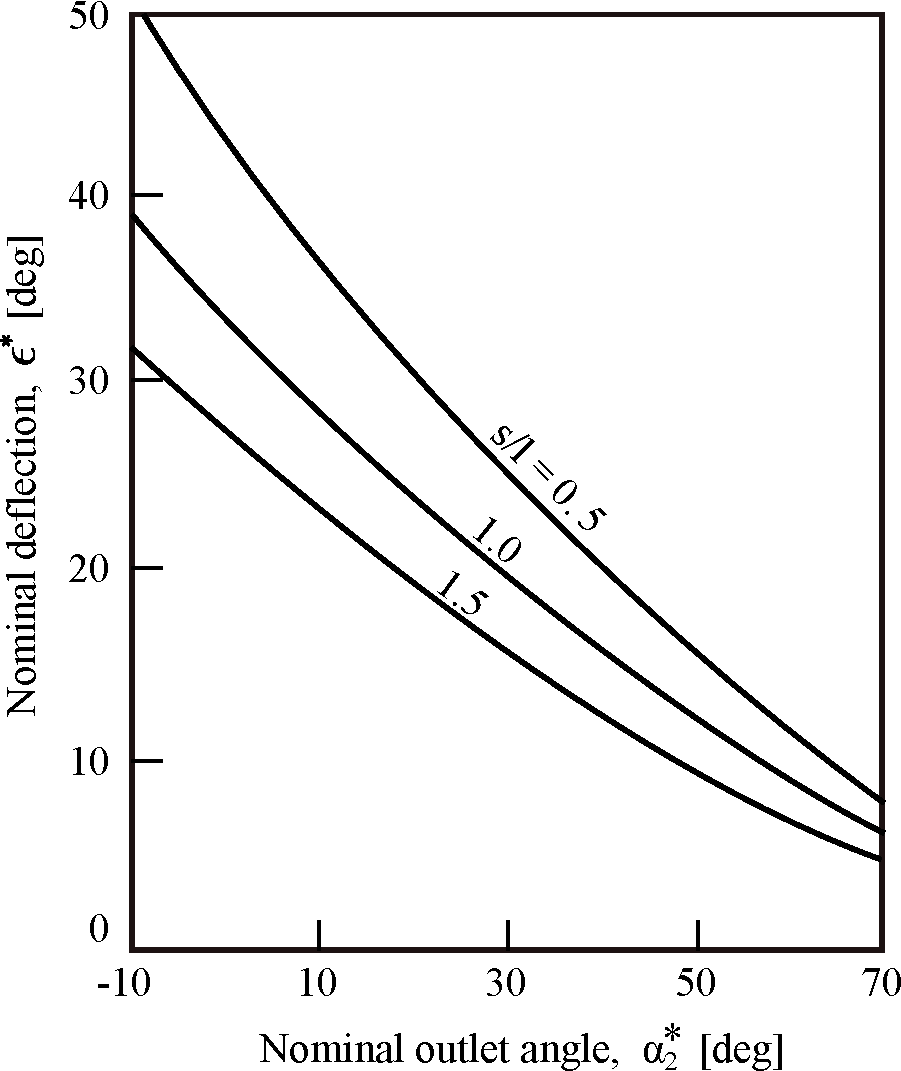
\includegraphics[width=.4\textwidth]{fig/1CorrHowell.pdf}
	\caption{Prima correlazione di Howell, $l$ è la corda del profilo}
	\label{fig:1CorrHowell}
\end{figure}
Se $ 20^{\circ} < \theta < 40^{\circ} $, la relazione della deflessione nominale è indipendente dall'angolo di deflessione geometrica $\theta$:
\begin{align*}
\varepsilon^* = f \bigg( \frac{s}{l}, \alpha_2^*, Re \bigg)
\end{align*}
e se $Re > 3 \cdot 10^5$, la correlazione diventa anche indipendente dal numero di Reynolds:
\begin{align*}
\varepsilon^* = f\bigg(\frac{s}{l}, \alpha_2^*\bigg)
\end{align*}
La deflessione nominale è definita come
\begin{align*}
\varepsilon^* = \alpha_1^* - \alpha_2^*
\end{align*}
e si può scrivere:
\begin{align*}
\boxed{\tan \alpha_1^* - \tan \alpha_2^* = \cfrac{1.55}{1 + 1.5 \cfrac{s}{l}}}
\end{align*}
valida nel range $0^\circ \leq \alpha_2^* \le 40^\circ$.

La seconda correlazione di Howell permette di trovare, noti gli angoli di flusso, i corrispondenti valori degli angoli geometrici della schiera ($\varepsilon = \varepsilon^*$). \'E possibile calcolare il valore della deviazione $\delta$ ossia lo scostamento tra angolo geometrico e angolo effettivo del flusso in uscita:
\begin{align*}
\delta = f \bigg( \theta, forma \; della \; pala, \frac{s}{l}, \gamma \bigg)
\end{align*}
con $\gamma$ angolo di calettamento. Si usa la seguente relazione, nota come legge di Costant:
\begin{align*}
\boxed{\delta^* = m \theta \bigg( \frac{s}{l} \bigg)^n}
\end{align*}
con $n = 1/2$ per schiere di compressore e $n = 1$ per schiere di IGV. Il coefficiente $m$ è funzione della forma della pala, in particolare della sua linea media (queste restano comunque delle correlazioni approssimative visto che derivano da osservazioni sperimentali):
\begin{align*}
m = 0.23 \cdot \bigg( 2 \cdot \frac{a}{l} \bigg)^2 + \frac{\alpha_2^*}{500}
\end{align*}
con $a$ che rappresenta la distanza del punto di massimo incurvamento della linea media rispetto il bordo d'ingresso. 

Con queste correlazioni si riducono i gradi di libertà nella definizione della geometria. Infatti una volta scelti $ \theta$ e $\sigma $, dalla seconda correlazione risulta $ \delta^* $ e dalla prima correlazione si trova $ \varepsilon^* $. In questo modo si definiscono:
\begin{align*}
i^* = \varepsilon^* - \theta + \delta^*
\end{align*}
\begin{align*}
\alpha_{1g} = \alpha_1^* - i^*
\end{align*}
\begin{align*}
\alpha_{1g} = \alpha_2^* - \delta^*
\end{align*}
e si può effettivamente disegnare la schiera. 

La terza correlazione di Howell permette di calcolare le prestazioni in off-design, quando $\varepsilon \neq \varepsilon^*$. Le condizioni di off-design possono verificarsi nel caso una macchina lavori in condizioni differenti da quelle nominali. In questi casi si va a rapportare la deflessione relativa $\varepsilon/\varepsilon^*$ rispetto ad altre caratteristiche.
\begin{figure}
\centering
  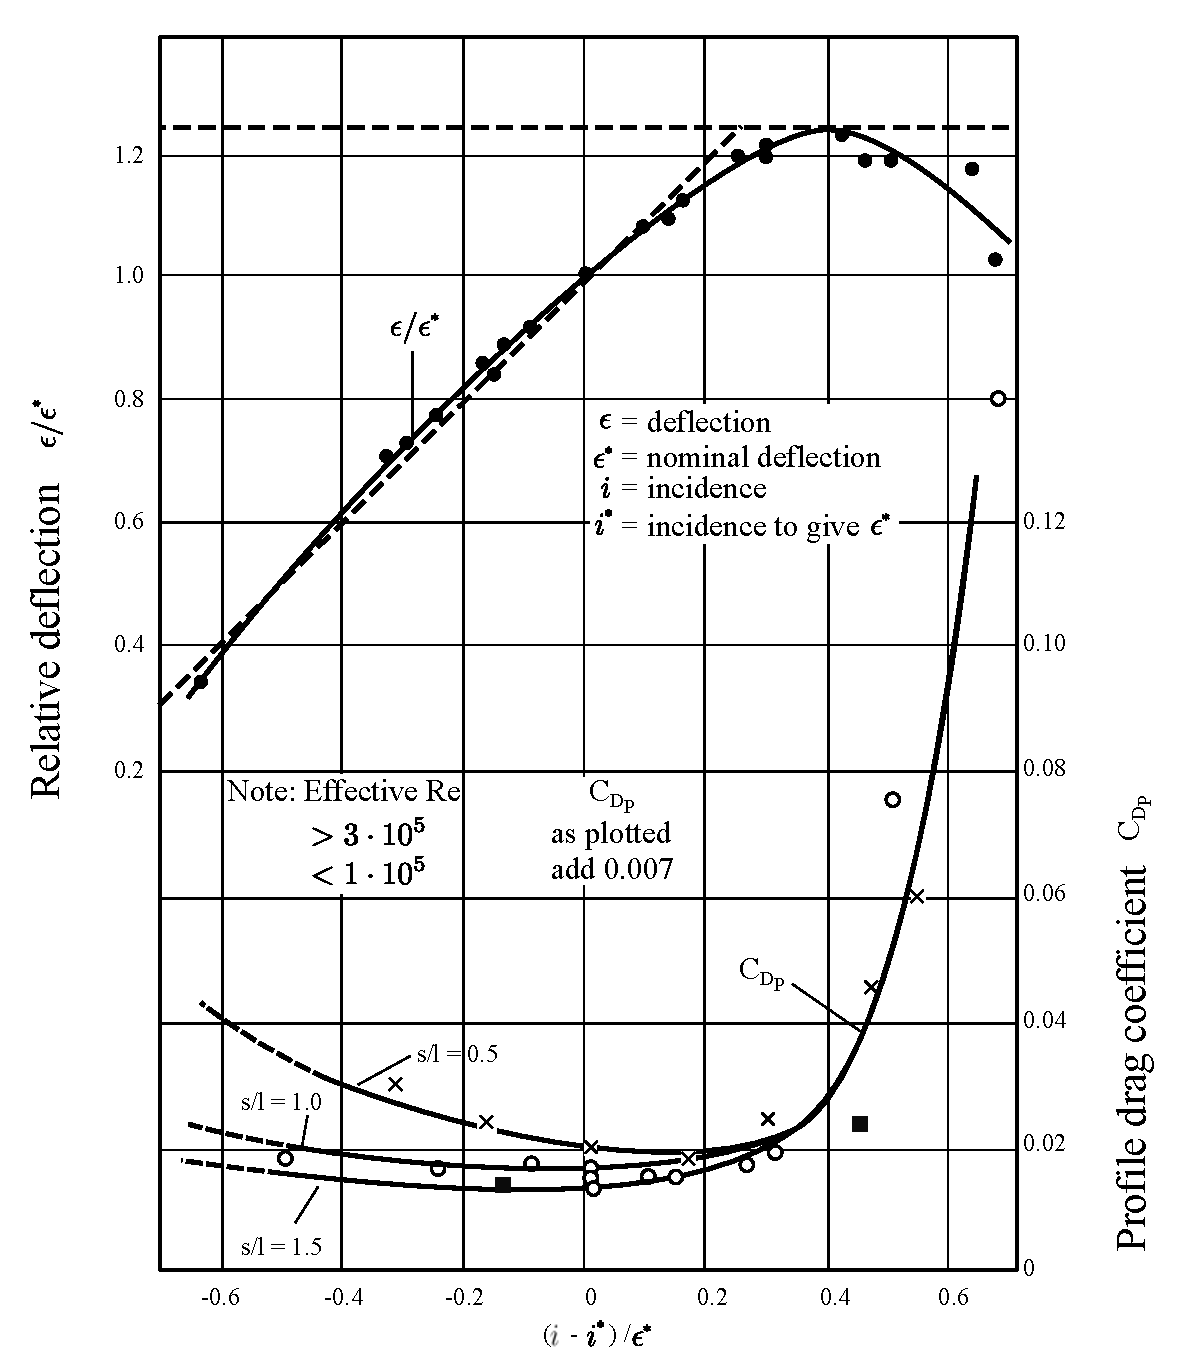
\includegraphics[width=0.8\textwidth]{fig/FuoriProg1.pdf}
\caption{}
\label{fig:FuoriProg1}
\end{figure}
Il diagramma in figura \ref{fig:FuoriProg1} permette di stimare il coefficiente di perdita $c_{Dp}$ e di considerare eventuali campi di variazione di Re differenti da quelli studiati nelle precedenti correlazioni; le curve vengono espresse a differenti valori di solidità.\\
In figura \ref{fig:FuoriProg2} si rapporta il coefficiente di incremento di pressione e il numero di Mach in entrata per una schiera con le caratteristiche riportate in figura; in questo modo è possibile avvicinarsi alle condizioni soniche e considerare anche i fenomeni di comprimibilità.
\begin{figure}[h!]
\centering
\begin{minipage}{.6\textwidth}
  \centering
  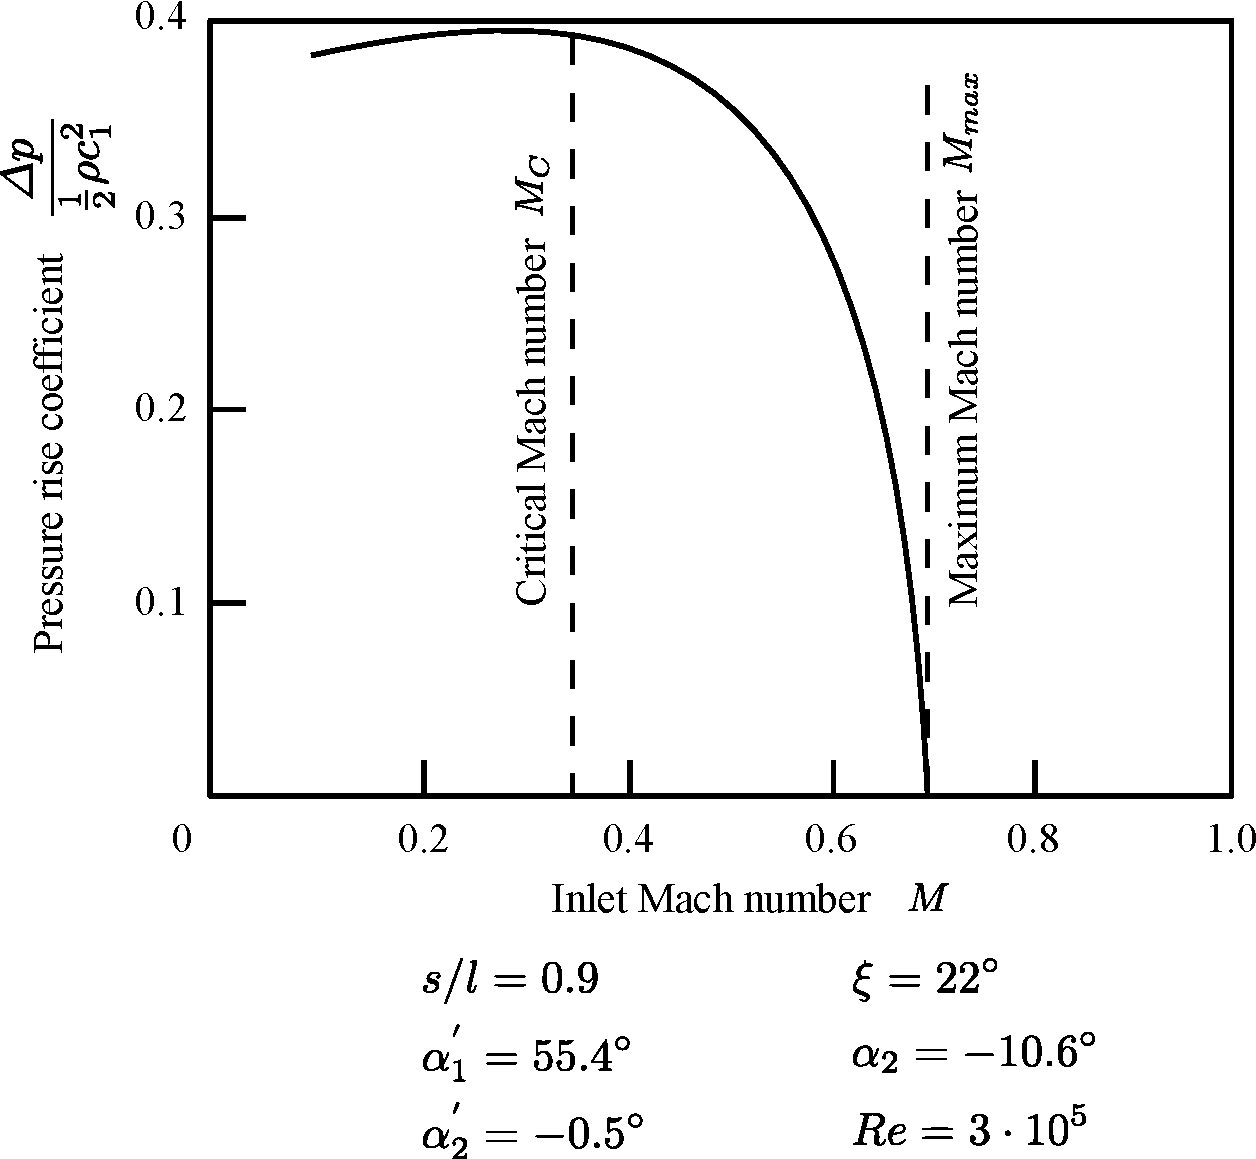
\includegraphics[width=.95\linewidth]{fig/FuoriProg2.pdf}
  \captionof{figure}{}
  \label{fig:FuoriProg2}
\end{minipage}%
\begin{minipage}{.4\textwidth}
  \centering
  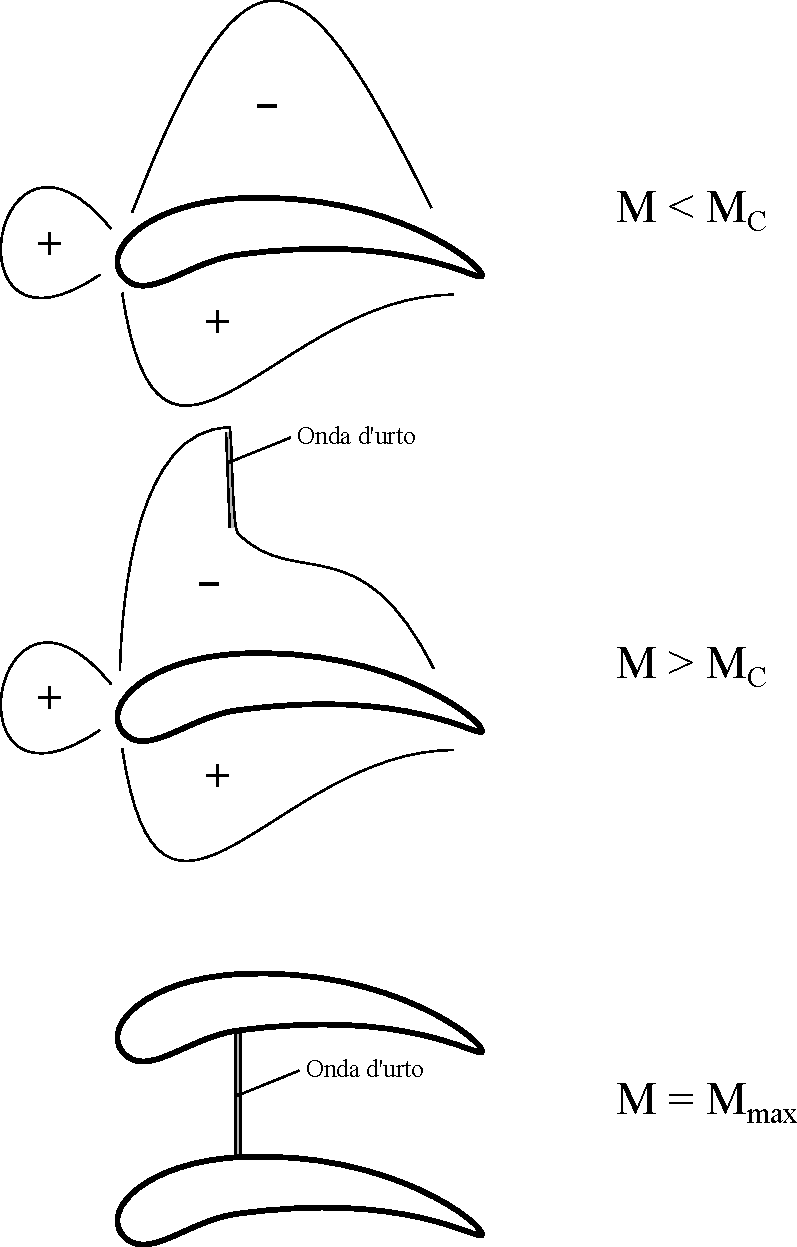
\includegraphics[width=.95\linewidth]{fig/FuoriProgMach.pdf}
  \captionof{figure}{ Campo di pressione attorno al profilo al variare del numero di Mach}
  \label{fig:FuoriProgMach}
\end{minipage}
\end{figure}
\\Finchè Ma resta basso il coefficiente di recupero di pressione non dipende da Ma. Raggiunto il valore di $M_{critico}$ il coefficiente di recupero di pressione diminuisce e c'è la possibilità che si formi un'onda d'urto con un decadimento delle prestazioni della schiera fino ad arrivare al loro annullamento in corrispondenza di $M_{max}$; in quest'ultima condizione in particolare, si ha un'onda d'urto che occupa l'intero condotto, quindi con condizioni di chocking, e di conseguenza la portata non può variare. La maggior parte dei test sperimentali che vengono svolti hanno lo scopo di trovare $M_c$.
\begin{figure}[h!]
	\centering
	\begin{minipage}{.6\textwidth}
		\centering
		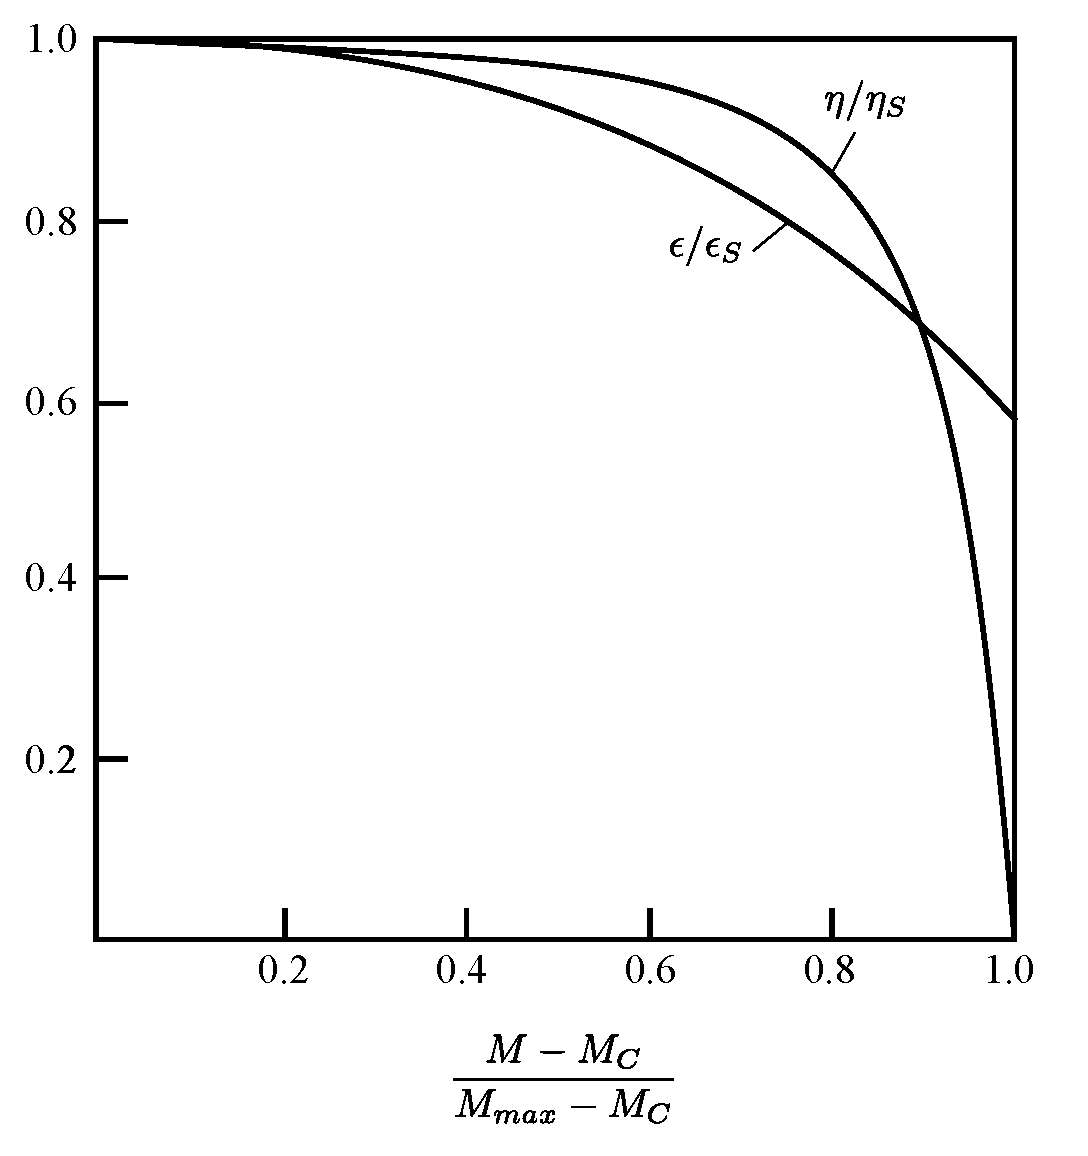
\includegraphics[width=\linewidth]{fig/FuoriProg3.pdf}
		\captionof{figure}{}
		\label{fig:FuoriProg3}
	\end{minipage}%
	\begin{minipage}{.4\textwidth}
		\centering
		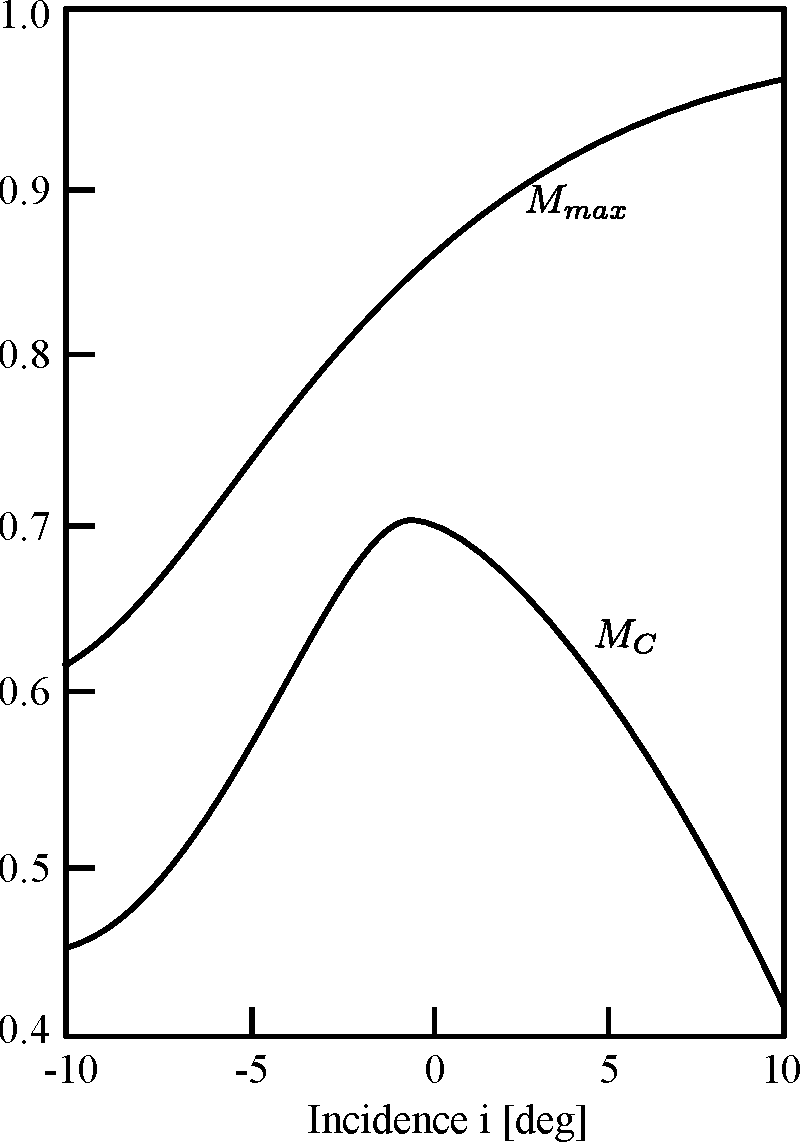
\includegraphics[width=\linewidth]{fig/FuoriProg4.pdf}
		\captionof{figure}{}
		\label{fig:FuoriProg4}
	\end{minipage}
\end{figure}
\\In figura \ref{fig:FuoriProg3} sono riportate le relazioni che correlano deflessione della schiera e il rendimento in funzione di una grandezza dipendente da $M$, $M_C$ e $M_{max}$ (sono valori specifici per condizioni fissate). \'E possibile notare dalla figura \ref{fig:FuoriProg4} come soprattutto $M_C$ sia pesantemente influenzato dall'angolo di incidenza.

\subsection{Criterio di carico}
Al variare del numero di pale ma a parità di lavoro svolto dalla macchina, si dovranno imporre diverse deflessioni con un conseguente carico diverso sulla singola pala: con poche pale si dovranno imporre deflessioni maggiori che portano ad un forte carico sul singolo profilo.\\
Si fa quindi una verifica: fissata la schiera e la solidità, si calcola il coefficiente di deflessione locale, $D_{loc}$, che indica quant'è la massima decelerazione a cui è soggetta la schiera:
\begin{equation}\label{eq:D_loc}
D_{loc} = \frac{V_{max} - V_2}{V_{max}}
\end{equation}
Si considera poi la riduzione di quantità di moto integrando sullo spessore occupato dalla scia:
\begin{equation}\label{eq:D_ridqmot}
\theta = \int_{\delta_P}^{\delta_S} \frac{\nu}{V} \bigg(1- \frac{\nu}{V} \bigg) dy
\end{equation} 
con $V$ è velocità di riferimento e $\nu$ velocità come funzione della posizione.
\begin{figure}
\centering
  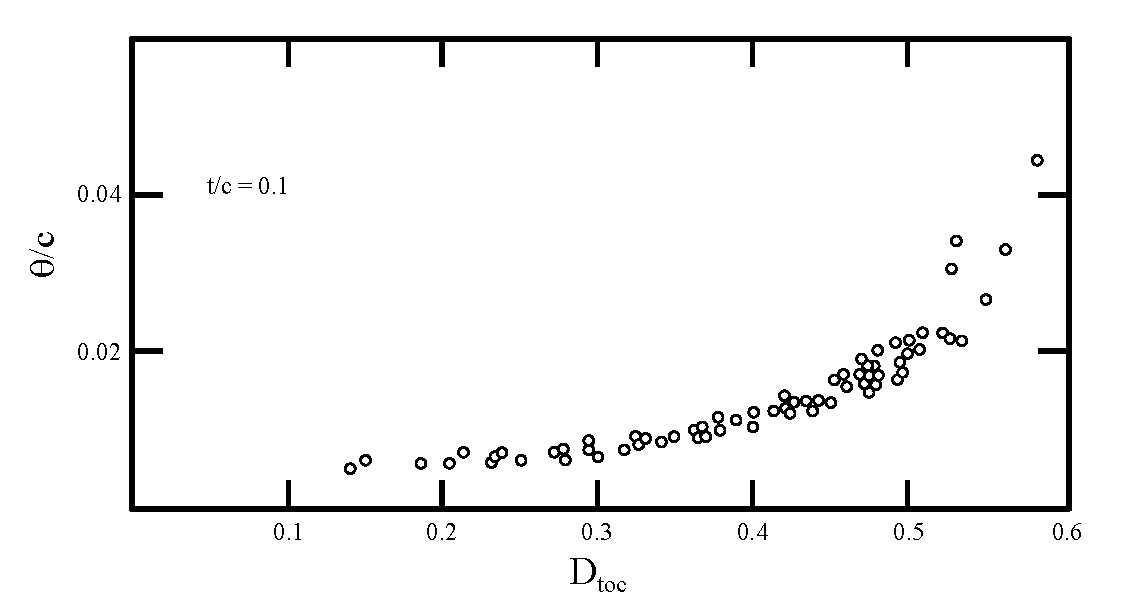
\includegraphics[width=\textwidth]{fig/CritCarico1.pdf}
\caption{}
\label{fig:CritCarico1}
\end{figure}
\begin{figure}
\centering
  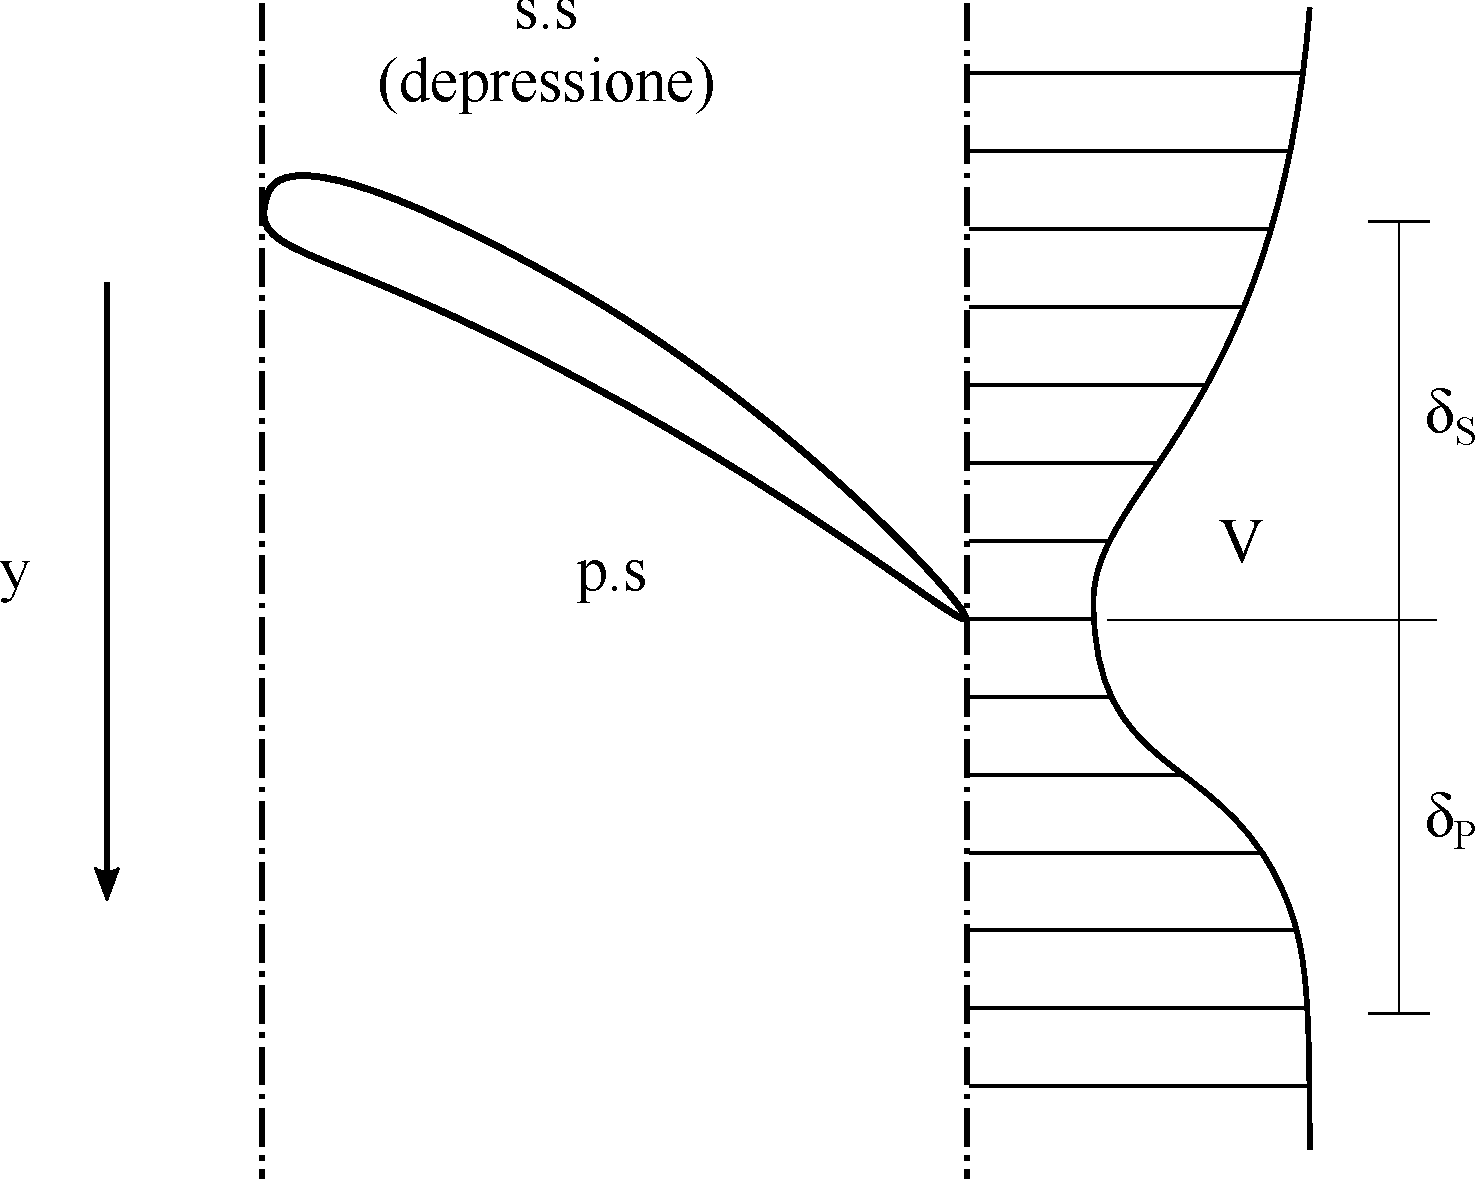
\includegraphics[width=.4\textwidth]{fig/CritCarico2.pdf}
\caption{}
\label{fig:CritCarico2}
\end{figure}
Se sono presenti molte pale, l'integrale diventa molto grande perché l'intero canale palare potrebbe essere occupato dalla scia, quindi come criterio empirico si utilizza:
\begin{align*}
\frac{\theta}{c} < 0.2
\end{align*}
In questo modo l'inspessimento di strato limite è considerato trascurabile rispetto alla corrente principale. 
\begin{figure}
\centering
  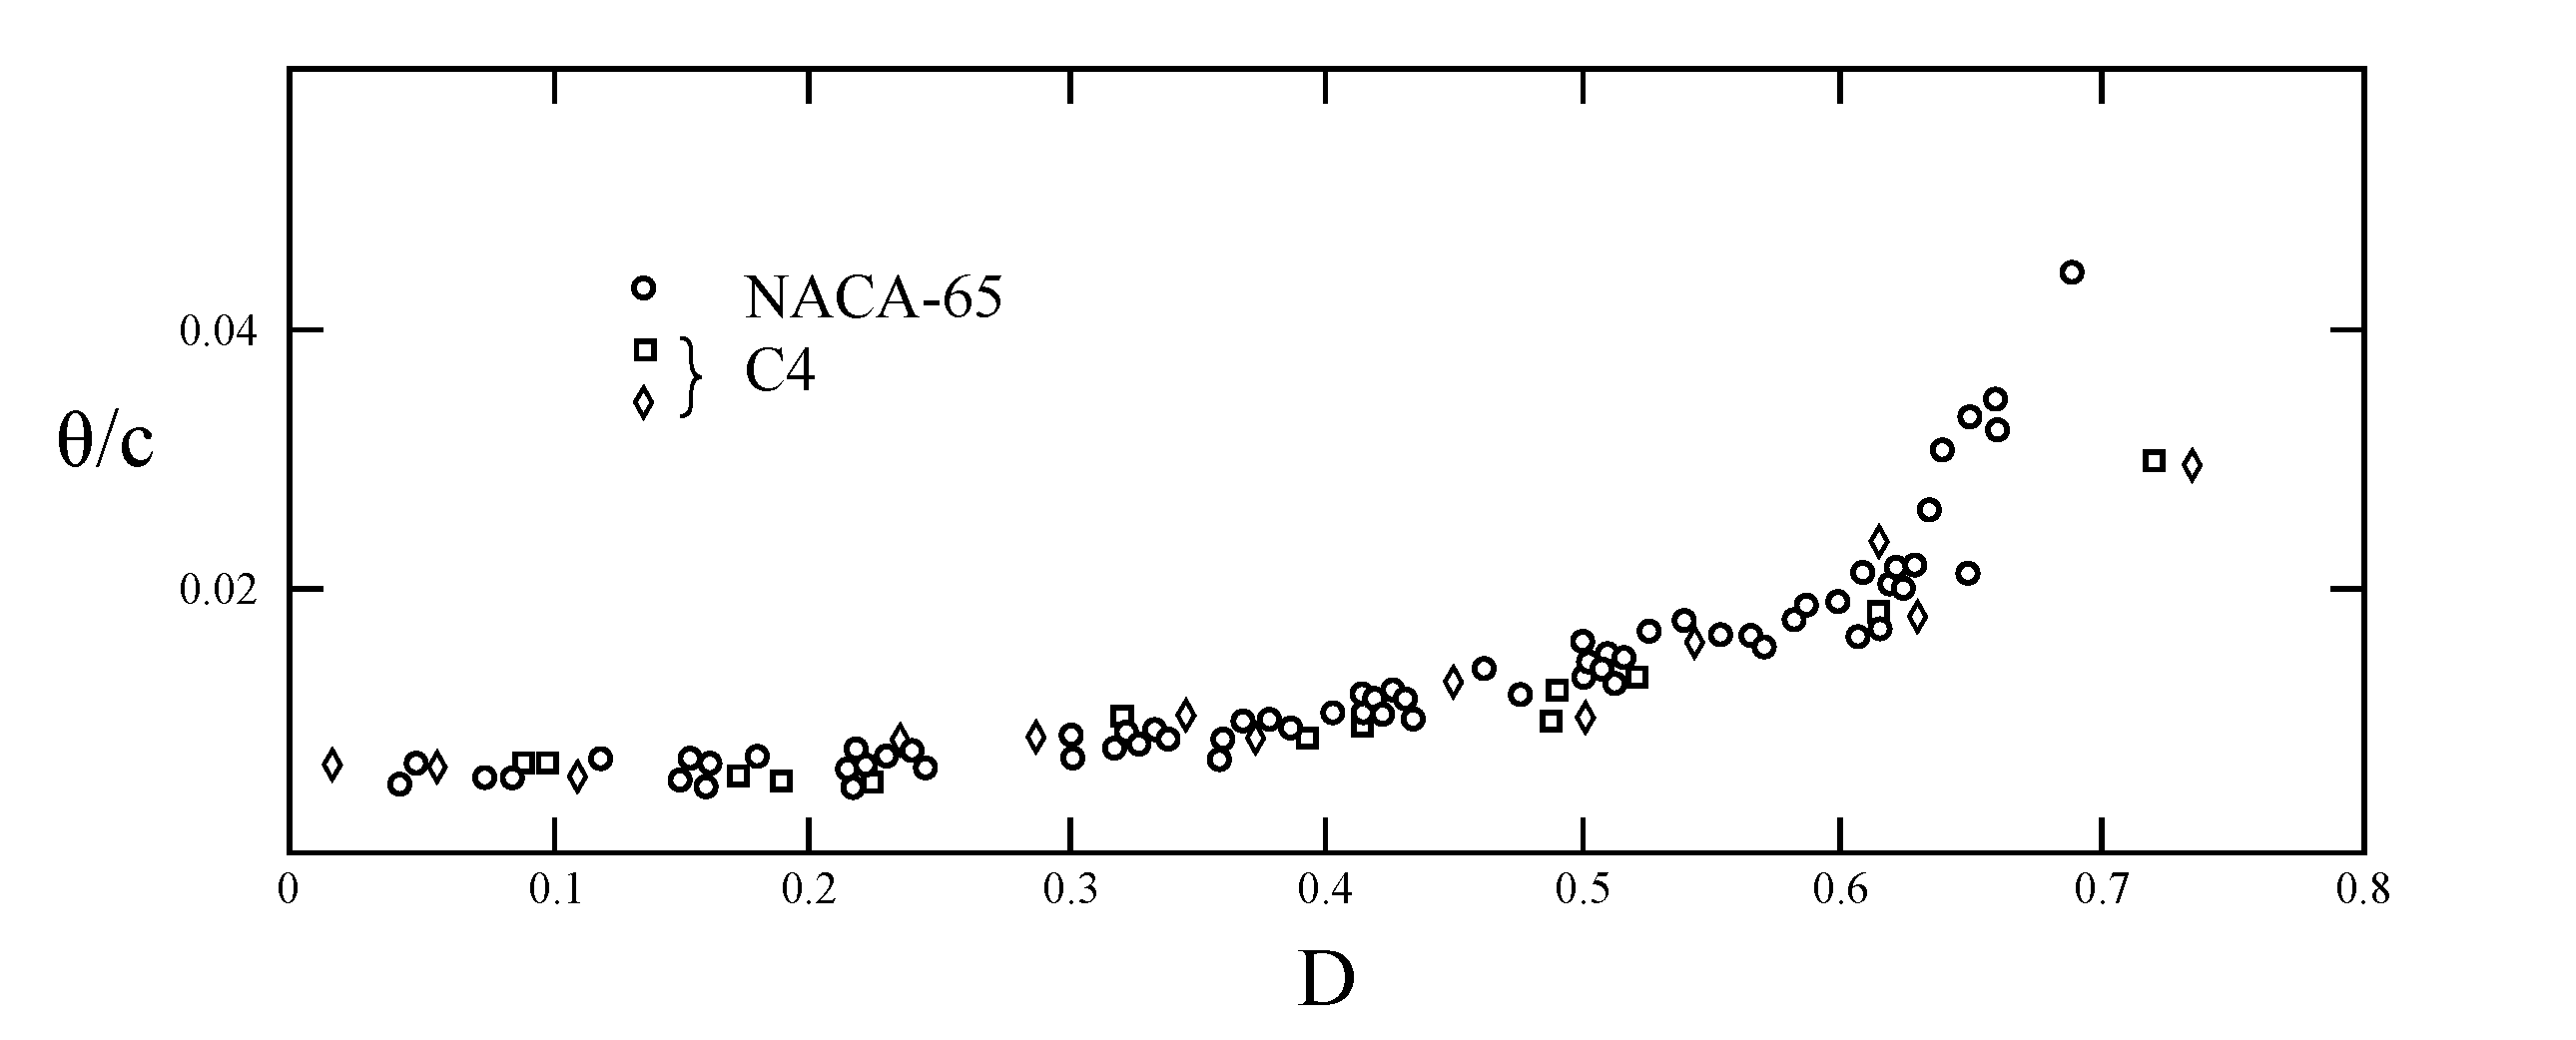
\includegraphics[width=\textwidth]{fig/CritCarico3.pdf}
\caption{}
\label{fig:CritCarico3}
\end{figure}
\\\'E possibile calcolare un fattore di diffusione globale, $D$, attraverso differenti correlazioni ottenute a partire da dati sperimentali (figura \ref{fig:CritCarico3}):
\begin{align*}
D = \bigg( \frac{V_1 - V_2}{V_1} \bigg) + \bigg( \frac{V_{t1} - V_{t2}}{2 \sigma V_1} \bigg) = \bigg( 1 - \frac{\cos \alpha_1}{cos \alpha_2} \bigg) + \frac{\cos \alpha_1}{2 \sigma} (\tan \alpha_1 - \tan \alpha_2)
\end{align*}
e come criterio empirico si usa $ D \leqslant 0.4 \div 0.5  $.
\begin{figure}
\centering
  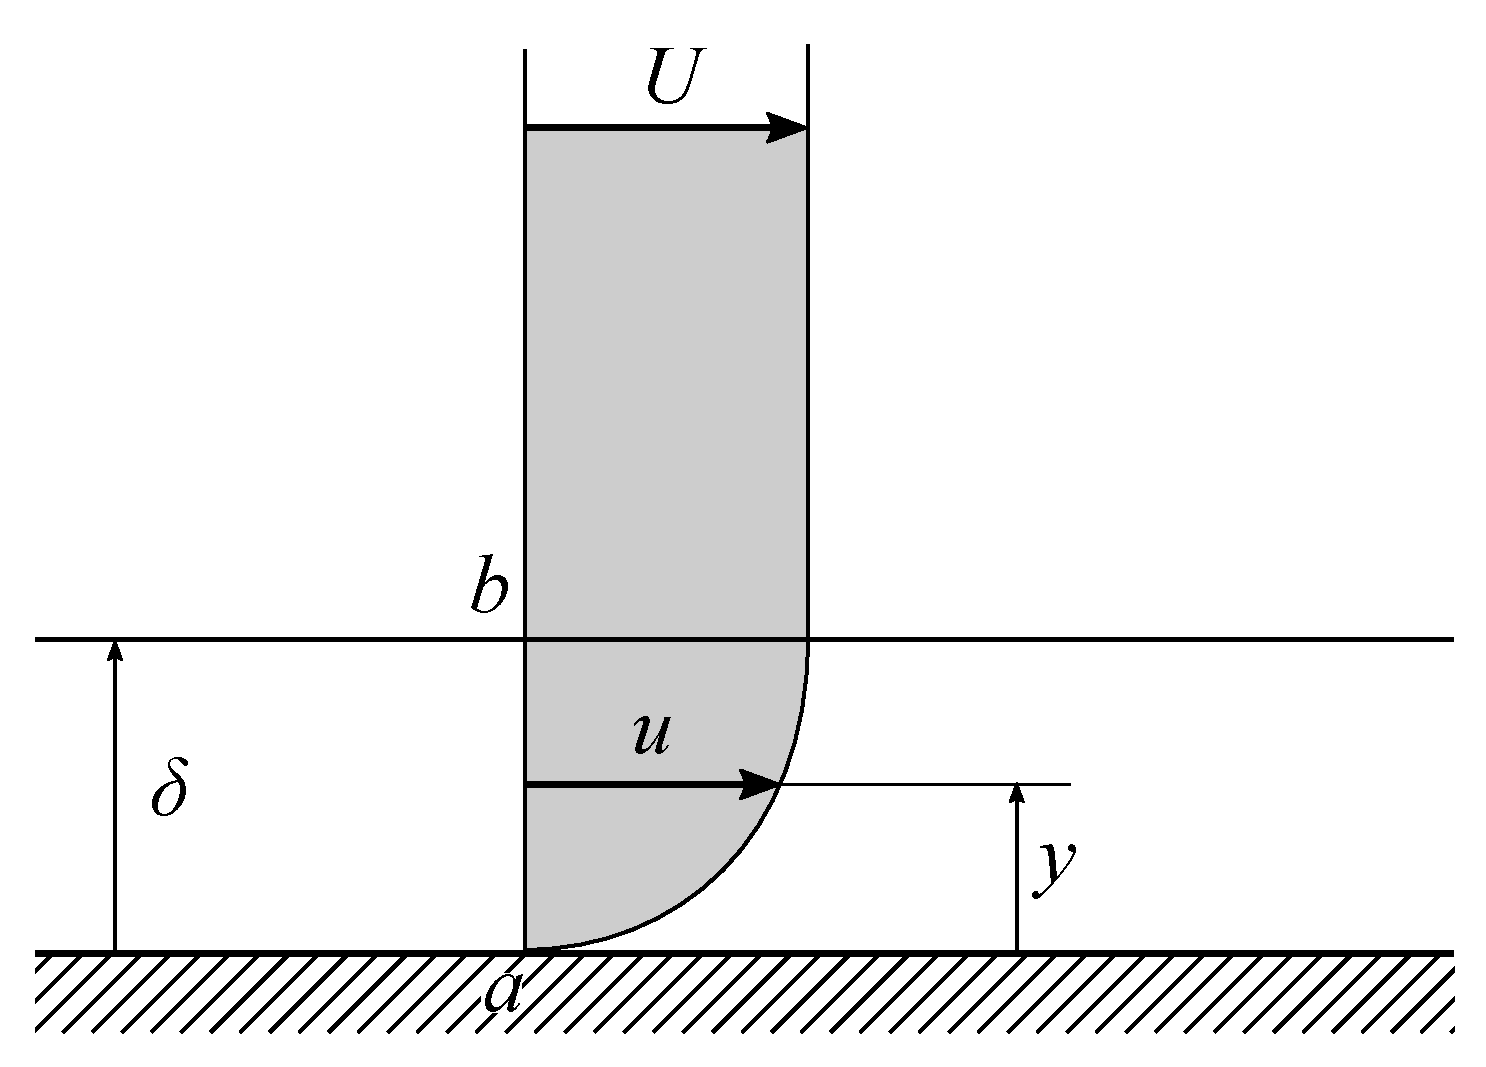
\includegraphics[width=.4\textwidth]{fig/CritCarico4.pdf}
\caption{}
\label{fig:CritCarico4}
\end{figure}
\\Infine si possono andare a cercare correlazioni rispetto allo strato limite come mostrato in figura \ref{fig:CritCarico4} e calcolare il decremento della quantità di moto come 
\begin{align*}
\Delta M = \int_0^{\delta} \rho u dy (U-u) = \rho \int_0^{\delta} u (U-u) dy
\end{align*} 
Quest'ultima fase però attualmente non ha molto senso in quanto questa è la parte di progettazione che si effettua per via numerica. A partire da questo decremento, è possibile calcolare lo spessore della quantità di moto dello strato limite al fine di valutare l'intensità energetica della scia in termini di perturbazione:
\begin{equation}
\theta = \frac{\Delta M}{\rho U^2} = \int_0^{\delta} \frac{u}{U} \bigg( 1 -\frac{u}{U} \bigg) dy
\end{equation}

\section{Schiere supersoniche}
Fin'ora si sono analizzate schiere di compressori con deflusso subsonico debolmente comprimibile con rapporti di compressione modesti ($10 \div 20 \%$) e con le seguenti condizioni sulla velocità in ingresso e in uscita:
\begin{align*}
\begin{cases}
M_1 <1\\
M_2 <1
\end{cases}
\end{align*} 

Si analizzano ora delle condizioni diverse in cui si presenteranno condizioni supersoniche. Questo tipo di deflusso consente un salto di pressione più elevato a scapito però di una pesante perdita in termini di rendimento. Queste trovano applicazioni particolari in campo aeronautico. 
\begin{itemize}
	\item Si parlerà di compressore transonico se:
	\begin{align*}
	\begin{cases}
	M_1 >1\\
	M_2 <1
	\end{cases}
	\end{align*} 
	Nel caso in cui si arrivi in condizione soniche all'interno della macchina si faranno ulteriori distinzioni rispetto alla componente assiale: 
	\begin{itemize}
		\item per $M_{1a} < 1 $ si parlerà di:
		\begin{itemize}
			\item \textit{regime non innescato} (figura \ref{fig:Schlieren1}a): è presente un'onda d'urto normale al flusso. Si avrà quindi una zona supersonica a monte e una subsonica a valle della schiera con un passaggio tra le due discontinuo; l'aumento di velocità è dovuto all'aumento di spessore della schiera;
			\item \textit{regime innescato} (figura \ref{fig:Schlieren1}b): la perturbazione di pressione occupa integralmente il condotto palare ed è distinguibile in maniera chiara (è comunque presente una zona subsonica in ingresso); la portata è bloccata; 
		\end{itemize}
		\item per $ M_{1a} > 1 $ si parlerà di \textit{regime saturo} (figura \ref{fig:Schlieren1}c): il blocco sonico è a monte della schiera dove si creano delle onde oblique che dissipano energia. Il deflusso in questo caso è complesso;
	\end{itemize}
	\item un'ulteriore possibilità, che però non ha rilevanza nei compressori, è:
	\begin{align*}
	\begin{cases}
	M_1 <1\\
	M_2 >1
	\end{cases}
	\end{align*} 
	In questo caso il flusso viene accelerato ma per definizione in un compressore si cerca esattamente l'effetto opposto;
	\item un ultimo caso è:
	\begin{align*}
	\begin{cases}
	M_1 >1\\
	M_2 >1
	\end{cases}
	\end{align*} 
	in cui il flusso è interamente supersonico ma non ha particolari interessi applicativi.
\end{itemize}
\begin{figure}[h!]
\centering
  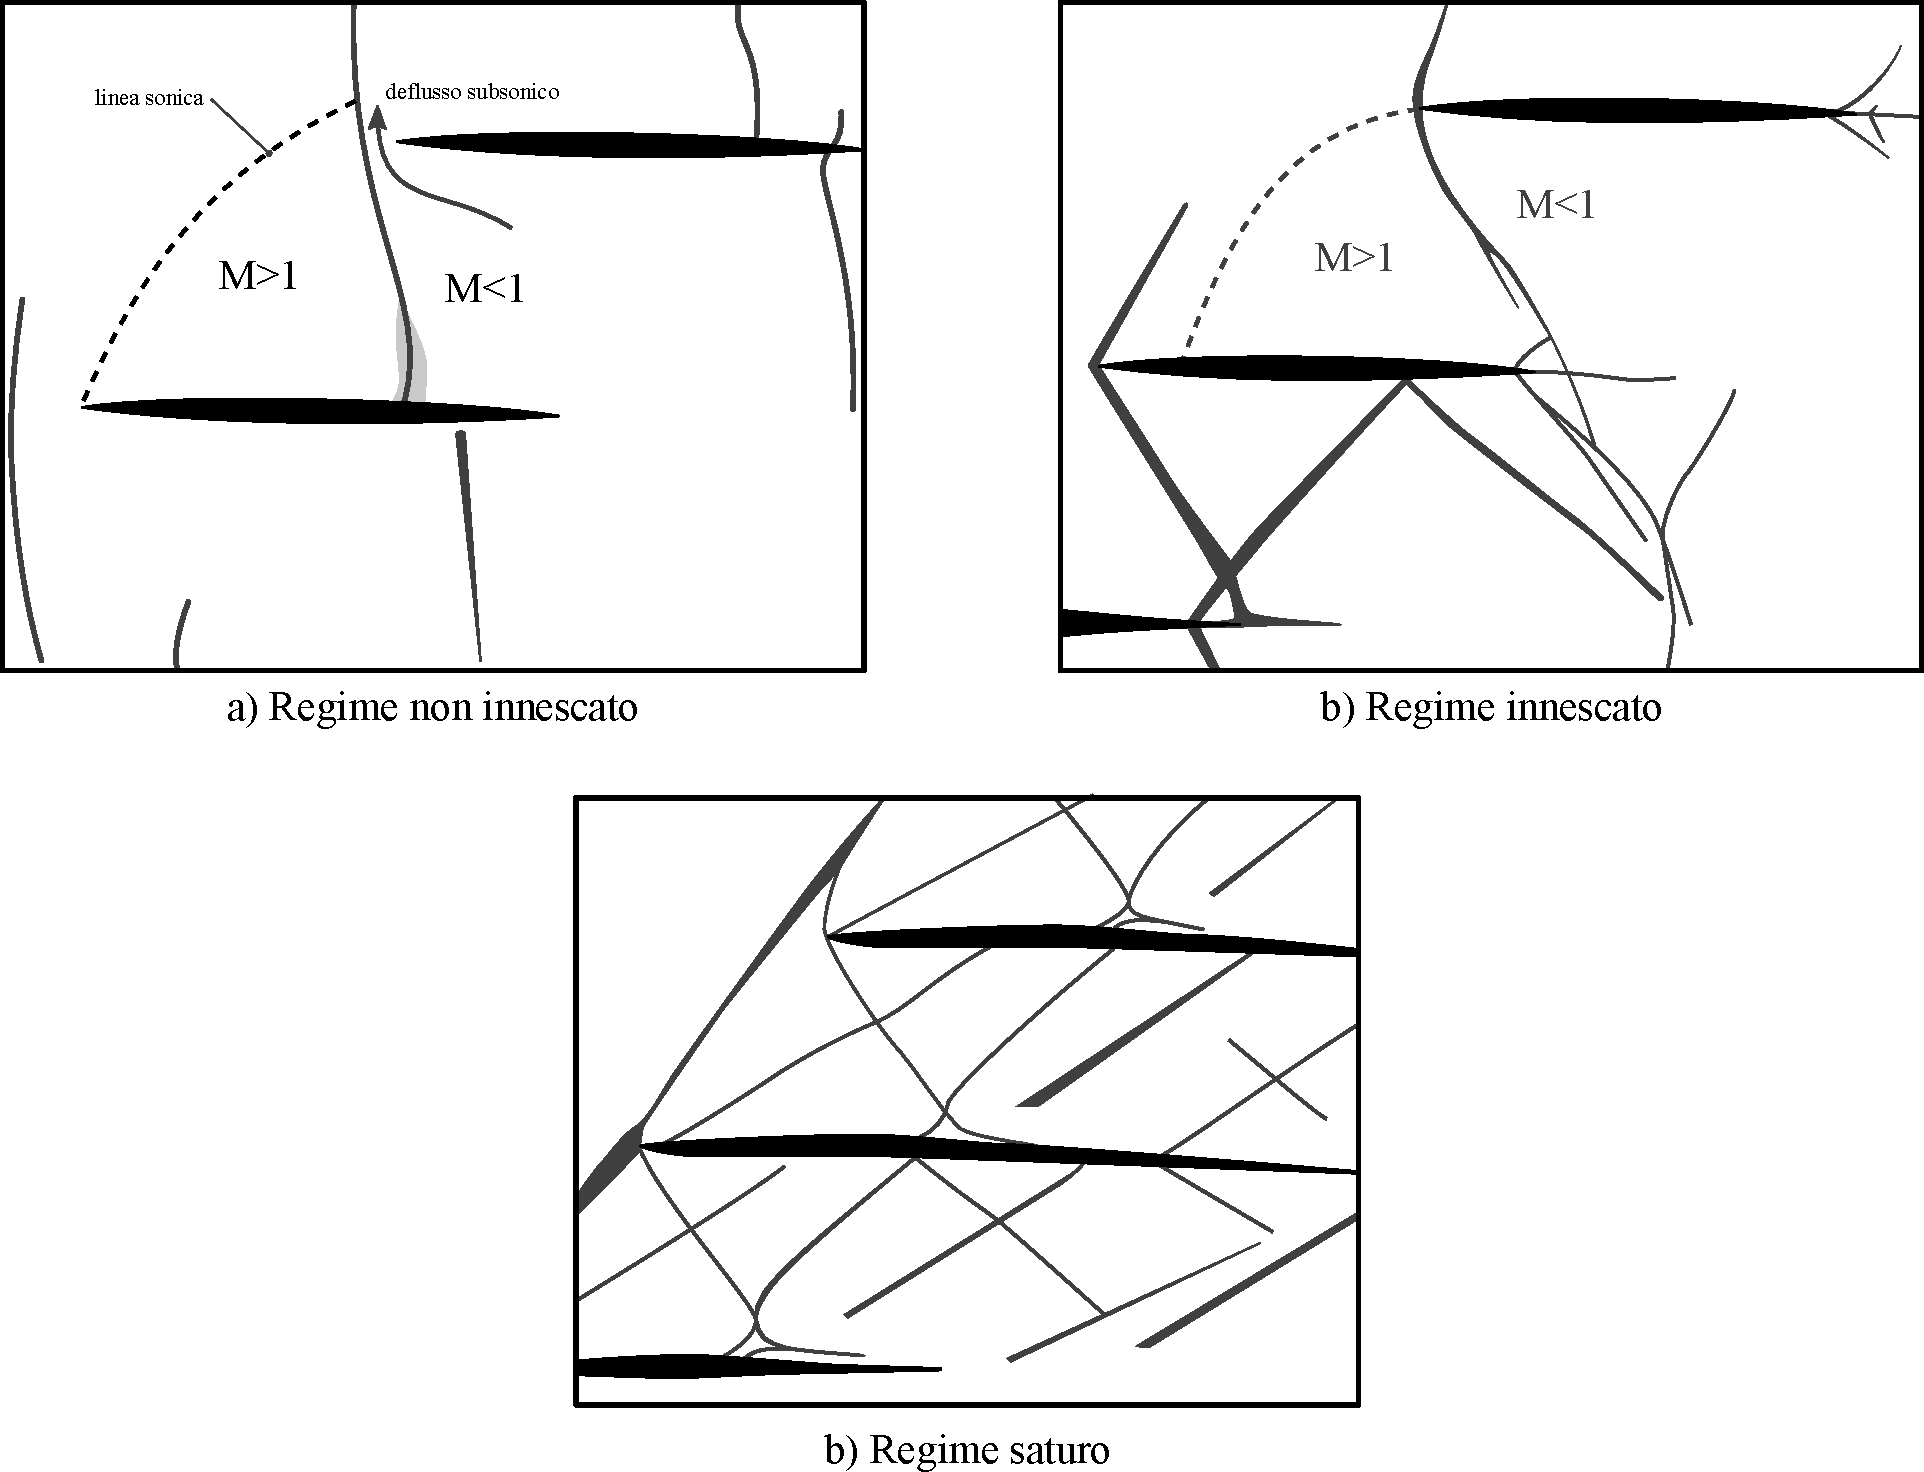
\includegraphics[width=.8\textwidth]{fig/Schlieren1.pdf}
\caption{}
\label{fig:Schlieren1}
\end{figure}
\begin{figure}[h!]
\centering
  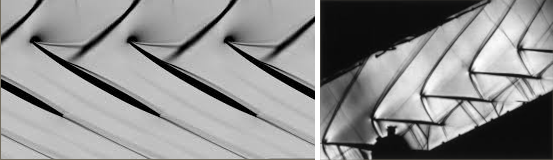
\includegraphics[width=.8\textwidth]{fig/Schlieren2.png}
\caption{}
\label{fig:Schlieren2}
\end{figure}


%\include{chapter}
%\appendix
%\include{appendix}

\backmatter%%%%%%%%%%%%%%%%%%%%%%%%%%%%%%%%%%%%%%%%%%%%%%%%%%%%%%%
%\include{Contenuto/solutions_it}
%%%%%%%%%%%%%%%%%%%%%%%%% referenc_it.tex %%%%%%%%%%%%%%%%%%%%%%%%%%%%%%
% Esempio di referenze
%
%
% Usare questo file come template per il vostro documento.
%
%%%%%%%%%%%%%%%%%%%%%%%% Springer-Verlag %%%%%%%%%%%%%%%%%%%%%%%%%%

%
% Utenti BibTeX: usare
% \bibliographystyle{}
% \bibliography{}
%
% Non-utenti BibTeX: usare
\begin{thebibliography}{[KLR73]}
%
% ed usare \bibitem per creare referenze.
%
% Usare la sintassi ed il markup seguenti per le vostre referenze.
%
% Monografie
\bibitem[KLR73]{monograph} Kagan, A.M., Linnik, Y.V., Rao, C.R.:
Characterization Problems in Mathematical Statistics. Wiley, New York (1973)

% Contributed Works
\bibitem[Mey89]{contribution} Meyer, P.A.: A short presentation of
stochastic calculus. In: Emery, M. (ed) Stochastic Calculus in
Manifolds. Springer, Berlin Heidelberg New York (1989)

% Journal
\bibitem[MR97]{journal} Miller, B.M., Runggaldier, W.J.: Kalman
filtering for linear systems with coefficients driven by a hidden Markov
jump process. Syst. Control Lett., \textbf{31}, 93--102 (1997)

% Tesi
\bibitem[Ros77]{thesis} Ross, D.W.: Lysosomes and storage diseases. MA
Thesis, Columbia University, New York (1977)

\end{thebibliography}

%\printindex

%%%%%%%%%%%%%%%%%%%%%%%%%%%%%%%%%%%%%%%%%%%%%%%%%%%%%%%%%%%%%%%%%%%%%%

\end{document}





